% - Week 1 is on the website: https://math216.wordpress.com/2020/06/27/discussion-for-this-week-starting-june-27-2020/
% - Week 2:https://math216.wordpress.com/2020/07/06/readings-and-problem-set-for-after-the-second-pseudolecture/
% - Week 3: https://math216.wordpress.com/2020/07/13/reading-and-problems-after-the-third-pseudolecture/
% Link to rising sea: https://math.stanford.edu/~vakil/216blog/FOAGnov1817public.pdf
% https://agittoc.zulipchat.com/
\documentclass{book}

% https://tex.stackexchange.com/a/97128
\usepackage[sc,osf]{mathpazo}   % With old-style figures and real smallcaps.
\linespread{1.025}              % Palatino leads a little more leading
% Euler for math and numbers
\usepackage[euler-digits,small]{eulervm}


\usepackage{mathtools}
\usepackage{amsmath}
\usepackage{amssymb}
\usepackage{amsthm}
\usepackage{minted}
\usepackage{hyperref}
\usepackage{tikz}
\usepackage{tikz-cd}
\usepackage{cancel}
\usepackage{mathtools}

% https://tex.stackexchange.com/questions/469588/strike-out-an-arrow-with-a-small-oblique-segment-like-with-nrightarrow
% \newcommand*\Neg[2][0mu]{\Neginternal{#1}{\negslash}{#2}}
% \newcommand*\sNeg[2][0mu]{\Neginternal{#1}{\snegslash}{#2}}
% \newcommand*\negslash[1]{\m@th#1\not\mathrel{\phantom{=}}}
% \newcommand*\snegslash[1]{\rotatebox[origin=c]{60}{$\m@th#1-$}}


\newcommand{\Hom}{\operatorname{Hom}}
\newcommand{\F}{\ensuremath{\mathcal{F}}}
\newcommand{\G}{\ensuremath{\mathcal{G}}}
\newcommand{\N}{\ensuremath{\mathbb{N}}}
\newcommand{\Z}{\ensuremath{\mathbb{Z}}}
\newcommand{\Q}{\ensuremath{\mathbb{Q}}}
\newcommand{\C}{\ensuremath{\mathbb{C}}}
\newcommand{\R}{\ensuremath{\mathbb{R}}}
\newcommand{\CP}{\ensuremath{\mathbb{CP}}}
\renewcommand{\P}{\ensuremath{\mathbb{P}}}
\newcommand{\A}{\ensuremath{\mathbb{A}}}
\renewcommand{\O}{\ensuremath{\mathcal{O}}}
\newcommand{\RP}{\ensuremath{\mathbb{RP}}}
\newcommand{\Spec}{\operatorname{Spec}}
\newcommand{\spec}{\operatorname{Spec}}
\newcommand{\m}{\mathfrak{m}}
\newcommand{\p}{\mathfrak{p}}
\newcommand{\q}{\mathfrak{q}}
\newcommand{\mSpec}{\m\operatorname{Spec}}
\newcommand{\mspec}{\m\operatorname{Spec}}
\newcommand{\frakp}{\ensuremath{\mathfrak{p}}}
\newcommand{\fraka}{\ensuremath{\mathfrak{a}}}
\newcommand{\coker}{\operatorname{coker}}
\newcommand{\colim}{\operatorname{colim}}
\newcommand{\inv}{\ensuremath{-1}}
\newcommand{\piinv}{\ensuremath{\pi^\inv}}
\renewcommand{\k}{\mathbb{k}} % field 
\newcommand{\pinv}{\piinv}
\newcommand{\piinverse}{\piinv}
\newcommand{\supp}{\operatorname{Support}}
\newcommand{\Set}{\ensuremath{\mathbf{Set}}}
\newcommand{\rad}{\sqrt} % radical
\renewcommand{\c}{\complement} % got tiring
\DeclarePairedDelimiter\ceil{\lceil}{\rceil}
\DeclarePairedDelimiter\floor{\lfloor}{\rfloor}
\DeclarePairedDelimiter\fracpart{\{}{\}}
\theoremstyle{definition}
\newtheorem{theorem}{Theorem}
\newtheorem{example}[theorem]{Example}
\newtheorem{aside}[theorem]{Aside}
\newtheorem{definition}[theorem]{Definition}
\newtheorem{exercise}[theorem]{Exercise}

%\newtheorem{proof}[theorem]{Proof}
\begin{document}
\tableofcontents
\chapter{Benedict gross, Lecture 30: Gaussian integers}
\begin{itemize}
    \item math e222 L30 20031201 
    \item \href{https://www.youtube.com/watch?v=itvvxpntpwg&list=PLelIK3uylPMGzHBuR3hLMHrYfMqWWsmx5&index=30}{YouTube link}
\end{itemize}
% math e222 L30 20031201 
\section{Recap: Euclidian Algorithm}
For any $a, b \in Z$ with $|b| < |a|$, we can decompose $a$ as
$a = \alpha \cdot b + r$ where $0 \leq r \lneq |d|$. This immediately implies
certain facts about the structure of ideals in \Z. 

\begin{theorem}
every ideal $I \neq 0$ in \Z~is principal. The generator of $I$
is the smallest positive integer in the ideal. Formally: $I = (\min\{ d \in I : d > 0 \})$.
\end{theorem}


\begin{proof}
Let $i \in I$ be a general element. Find its decomposition into $d$ using the
Euclidian algorithm as $i = \alpha \cdot d + r$.
Reasoning by ideals:

\begin{align*}
&\forall i \in I, \exists \alpha, r \in \Z, |r| \lneq d, \quad i = \alpha \cdot d + r \\
&\{ \text{writing in ideal notation,} \} \\
&\exists r \in \Z, r \not \in I,  \quad I \subseteq Z \cdot d + r \\
&\{ \text{since $I = (d)$,} \} \\
&\exists r \in Z, r \not \in \Z, \quad I \subseteq  I + r \\
&\implies r = 0
\end{align*}
\end{proof}

\begin{theorem}
Ideal $I = (a, b)$ is a principal ideal $I = (gcd(a, b))$.
\end{theorem}
\begin{proof}
We already know that every ideal $I$ is generated by its smallest positive number $d$.
We will show that $d = gcd(a, b)$. We first show that $d$ is a divisor of $a$, and
a divisor of $b$.
Since $a \in (a, b) = I = (d)$, we know that $a = \alpha \cdot d$
for some $\alpha \in \Z$. Hence $d$ divides $a$. Similarly, $d$ divides $b$.
To show that $d$ is the \emph{greatest common divisor}, let there be another
divisor common divisor $d'$ which divides $a$ and $b$:

\begin{align*}
& d \in I = (a, b) \implies d = ma + nb \quad \text{(Any element in $I$ can be written as $ma + nb$)} \\
&d' | a \implies d' | m a,d' | b \implies d' | n b \\
&d' | m a \land d' | n b \implies d' | [(m a + n b) = d]\\
& d' \leq d \quad \text{(A divisor of a number must be less than or equal to the number)}
\end{align*}             

Hence, $d = gcd(a, b)$.
\end{proof}


\begin{theorem}
If $p$ is a prime and $p | ab$ then $p | a$ or $p | b$.
\end{theorem}
\begin{proof}
We know that $gcd(a, p) = p \lor gcd(a, p) = 1$, since the only divisors of
$p$ are 1 and $p$ itself. If $p | a$ then we are done.
If $p \not| a$, then $gcd(a, p) \neq p$, and we must have $gcd(a, p) = 1$.
This means that $1 = \alpha a + \beta p$. Multiplying throughout by $b$, 
we get that $b = \alpha (ab) \beta (pb)$. We know that $p | ab$, and clearly
$p | pb$. Hence, we must have that $p|(ab + pb)$. Therefore, $p|b$.
\end{proof}


\begin{theorem}
Every integer $z$ has a unique decomposition into a product of primes of
the form ${z = \pm p_1 p_2 \dots p_n}$.
\end{theorem}
\begin{proof}
Proof by induction on the number of factors and using the property that if
$p|ab \implies p|a \lor p|b$. We prove this by induction on the size of
the number. It clearly holds for $2$ since $2$ is prime. Now, let us assume
it holds till number $n$. Now we consider $(n+1)$. If $(n+1)$ is prime,
then the decomposition is immediate. Assume it is not. This means that
$(n+1) = \alpha \beta$, for $\alpha, \beta \leq n$. We know that $\alpha, \beta$
have unique factorization. We can easily show that the product of two unique
factorizations also has a unique factorization. Hence proved.
\end{proof}

So really, given the Euclidian algorithm, we get this kind of prime decomposition
and the unicity of factorization.

\section{$\Z[i]$: The Gaussian integers}
The size function is the absolute value $\delta(a+bi) \equiv |a+bi|^2 = a^2 + b^2$.
A corollary of this is that every ideal of $Z[i]$ is principal. In particular,
the ideal $I_p$ such that $\Z[i]/I_p \simeq \Z/p\Z$ where $p \equiv 1 \mod 4$ is
principal, and is generated by a single element $a_p + b_p i$, and also that
$a_p^2 + b_p^2 = p$. This is Fermat's theorem, which shows that every
prime $p \equiv 1 \mod 4$ can be written as a sum of squares.

\section{$\delta(r) = |r|$ is a size function}

Let's try to show that $\delta$ is a good size function. Let us pick $B, A \in \Z[i]$.
We can write $B = A \cdot w$, where $w = \alpha + \beta i$ where $\alpha, \beta \in \Q$.
This is easy to do because in the complex numbers, we know that $B/A = B\bar{A}/(A\bar{A})$,
where $\bar A$ is the complex conjugate.  Hence $w = B/A = B\bar{A}/(A\bar{A})$.
We split $\alpha, \beta$ into their integer and fractional parts by
writing $\alpha = \alpha_0 + r_0$, $\beta = \beta_0 + s_0$ where
$\alpha_0, \beta_0 \in \Z$ and $-1/2 \leq r_0, s_0 < 1/2$. This gives us:

\begin{align*}
B = Aw = A(\alpha + \beta i) = A(\floor{\alpha} + i \floor \beta) + A(r_0 + s_0 i) \\
\end{align*}
Note that $A(\floor{\alpha} + i \floor \beta) \in \Z[i]$. What
we have leftover is $r \equiv A(r_0 + s_0 i)$, the remainder. 
We claim that $\delta(r) < \delta(A)/2$. To prove this, we note that $\delta$
which is the absolute value is multiplicative: $\forall u, b \in \C, |ub| = |u||b|$.
Hence, we get that $\delta(Ar) = \delta(A)\delta(r) = \delta(A)(r_0^2 + s_0^2)$.
Hence we can conclude that:

\begin{align*}
& \delta(Ar) = \delta(A)(r_0^2 + s_0^2) \leq \left[ \delta(A)(1/2^2 + 1/2^2) = \delta(A)(1/4 + 1/4) = \delta(A)/2 \right] \\
& \delta(Ar) \leq \delta(A)/2
\end{align*}

Note that the above trick of writing things in terms of $\alpha + \beta i = (\alpha_0 + \beta_0 i) + (r_0 + s_0i)$
does not allow us to show that all rings of the form \Z~with stuff adjoined is Euclidian. For
a concrete non-example, take $\Z[\sqrt{-5}]$. Here, the factorization works
out to be $(r_0 + 5 s_0 i) \leq 1/4 + 5/4$ which \emph{does not decrease} the
size. More drastically, $Z[\sqrt{-5}]$ cannot be a Euclidian domain for any
choice of size function, since unique factorization fails. $6 = 2 \times 3 = (1+ \sqrt{-5})(1-\sqrt{-5})$.

\chapter{Benedict gross, Lecture 31: Gaussian integers}
\begin{itemize}
    \item \href{https://www.youtube.com/watch?v=l1OWAasmBLI&list=PLelIK3uylPMGzHBuR3hLMHrYfMqWWsmx5&index=31}{YouTube link}
\end{itemize}

\section{Goals for the leture}

General version: If $R$ is a domain with unique factorization into primes, then so is $R[X]$.

What we will show: $\Z[X]$ has unique factorization even though it is not a PID.
Why is it not a PID? If it were a PID, then prime ideals are maximal. The ideal $(X)$
is prime, but the quotient $\Z[X]/(X) \simeq \Z$ is not a field, hence $(X)$
is not maximal though $(X)$ is prime. Thus $\Z[X]$ is not a PID.

We will show that $\Z[X]$ still has unique factorization even though it is
not a PID.

\section{Investigating factorization in $\Z[x]$}

Let's start off with $f(x) \in \Z[x] \subset \Q[x]$. So if we go to $\Q[x]$,
we can definitely factor more polynomials than we could over $\Z[x]$.

We write $f(x) = c \cdot p_1(x) \cdot p_2(x) \dots p_n(x)$, where each
of the $p_i(x)$ are monic irreducible in $\Q[x]$, and $c \in \Q^x$ is a unit.
This factorization is unique because $\Q[x]$ is euclidian, and is thus
PID, and is thus a UFD (unique factorization).


For example, if we take $f(x) = 2x+1$, in the unique factor form, we would
write it as $f(x) = 2(x + 1/2)$ since we need a monic polynomial. But we
don't have $1/2 \in \Z$, so we are hosed. The problem is that the factors
are not in $\Z[X]$.

We need to have a replacement of the notion of a monic polynomial over $\Z[X]$.
The analogue of a monic polynomial is what is called as a \textbf{primitive polynomial}.

\section{Primitive Polynomials}
A primitive polynomial has the form:

\begin{align*}
&f_0(x) \equiv  a_n x^n + \dots + a_0 ; a_i \in \Z \\
&\gcd(a_1, a_2, \dots, a_n) = 1 \\
&(a_1, a_2, \dots, a_n) = \Z \quad \text{ideal generated by them is $\Z$}
\end{align*}

Note that the ideal based condition allows us to multiply by $-1$ (ie, flip all signs) 
and still keep that $(a_1, a_2, \dots, a_n) = \Z$. To remove this degree of
freedom, we add the condition that $a_n > 0$.

\begin{theorem}
any polynomial $f$ over the integers can be written uniquely
as $f = c f_0$, where $c$ is an integer and $f_0$ is primitive. Formally,
for all $f \in \Z[x]$, we have $c \in \Z$ and $f_0 \in Z[X]$, $f_0$ primitive
such that $f = c f_0$.
\end{theorem}
\begin{proof}
    For a given $f$, pull out $c \equiv gcd(a_0, a_1, \dots, a_n)$. Factorize
    $f = c f_0$, by setting $f_0 \equiv f / c$. If leading coefficient of
    $f_0$, $a_n < 0$, then flip the signs: $(c \mapsto -c; f_0 \mapsto -f_0)$.
\end{proof}

\begin{example}
    If we have $f(x) = 6x^2 - 3x + 9$, then we get the factorization
    $f(x) = 3(2x^2 - x + 3)$.
\end{example}

What's nice is that we have such an expression for rational polynomials
as well! 

\begin{theorem}
If $f(x) \in \Q[x]$, we can write it as $f(x) = c f_0(x)$ where
$f_0(x)$ is primitive in $\Z[x]$, while $c \in \Q$. This expression is
\emph{unique}.
\end{theorem}
\begin{proof}
    Given a rational polynomial $f(x) \in \Q[x]$, first clear out all denominators,
    writing the polynomial as $1/n g(x)$ where $g(x) = nf(x)$, $g(x) \in \Z[x]$.
    Then write $g(x) = d f_0(x)$ for $d \in Z$, $f_0(x)$ primitive in $\Z[x]$.
    We then write $f(x) = 1/n g(x) = (d/n) f_0(x)$
\end{proof}

What is cool about this is that we can tell from this decomposition when
the polynomial is integral and when it is not.
\begin{theorem}
Let $f(x) \in \Q[x]$.
$f(x)  in \Z[x]$ iff when we write $f(x) = c f_0(x)$ for $f_0 \in \Z[X]$ and $c \in \Q$, we
have that $c \in \Z$. (Aside: This value $c$ is called as the \textbf{content} 
of the polynomial $f$).
\end{theorem}
\begin{proof}
    \textbf{forward: $f(x) \in \Z[x] \implies c \in \Z$}
    We have that $f(x) \in \Z[x]$. 
    we can write such a polynomial as $f(x) = c f_0(x)$ for $c \in \Q, f_0 \in \Z[x]$.
    Since the coefficients of $f(x)$, are the
    coefficients of $f_0$ times $c$, we have that $\Z = c \Z$, which
    implies that $c \in \Z$.

    \textbf{backward: $c \in \Z \implies f(x) \in \Z[x]$}
    We have that $f(x) = c f_0(x)$ for $c \in \Z, f_0 \in \Z[x]$.
    We already have $f_0 \in \Z[x]$. Multiplying the two
    out, we get that $f = c f_0 \in \Z[x]$, since the $i$th coefficient
    of $f$ is the $i$th coefficient of $f_0$ times $c$, both of which are in $\Z$.
\end{proof}

\section{Factorization of polynomials in $\Z[x]$}

Let's now take an $f(x) \in \Z[x] \subset Q[x]$. We first factorize it in $Q[x]$,
giving us $f(x) = c p_1(x) \dots p_n(x)$ with each $p_i(x)$ monic.
Now we write each $p_i = c_i q_i(x)$
[the primitive decomposition] with each $q_i(x)$ primitive.
This gives $f(x) = c c_1 q_1(x) c_2 q_2(x) \dots c_n q_n(x)$.
We now write this as $f(x) = d q_1(x) q_2(x) \dots q_n(x)$ where $d = c c_1 \dots c_n$.
We are now left with $q_i(x)$ where the $q_i(x) \in \Z[X]$. These $q_i(x)$
continue to be irreducible in $\Q[x]$. But our $d \in \Q$, since we have
$c_1, c_2, \dots c_n \in Q$. We need to show that this $d \in \Z$.

\section{Gauss' lemma}

\begin{theorem}
    If $f_0$ and $g_0$ are primitive polynomials, then so is $f_0 g_0$.
\end{theorem}
\begin{proof}
    If not, say that the prime $p$ divides all the coefficients of $f_0(x) g_0(x)$:
    By definition, the product is not primitive if the $\gcd$ of all the coefficients
    is not 1. Hence there exists some prime that divides all the coefficients.


    Consider the morphism $\phi: \Z[x] \rightarrow \Z/p\Z[x]$, which sends $f(x) = \sum_i a_i x^i$
    to $\overline{f}(x) = \sum_i \overline{a_i}x^i$.

    Since $p$ divides all the coefficients of $f_0 g_0$, we have that $\phi(f_0 g_0) = 0$.
    But this tells us that $\phi(f_0) \phi(g_0) = 0$. This means that either $\phi(f_0) = 0$
    or $\phi(g_0) = 0$ since $\Z/p\Z$ is a field. This means that either $f_0$
    or $g_0$ is not primitive, since $p$ divides their coefficients.
\end{proof}


\section{factorization of polynomials in $\Z[x]$: Redux}
Now that we are armed with Gauss' lemma, note that we had $f(x) \in \Z[x]$.
We wrote it as $f(x) = d q_1(x) \dots q_n(x)$ where each $q_i(x) \in \Z[x]$.
From gauss' lemma, we know that the product
$q(x) \equiv q_1(x) \dots q_n(x) \in \Z[x]$.
Hence we have that $\Z (f(x)) = \Q(d) \Z (q(x))$, and thus $d \in \Z$.


We also have that that these $q_i(x)$ are irreducible in $\Z[x]$. If there we
reducible in $\Z[x]$, then they are definitely reducible in $\Q[x]$. But this
cannot be, by construction.


Hence we obtain a factorization:

\begin{align*}
&f(x) \in Z[x] \\
&f(x) = c \prod_i p_i(x) \quad p_i(x) \in \Q[x]; c \in \Q \\
&f(x) = c \prod_i (d_i q_i(x)) \quad q_i(x) \in \Z[x]; c, d_i in \Q \\
&f(x) = d \prod_i q_i(x) \quad q_i(x) \in \Z[x]; d \in \Z (\text{Gauss lemma})\\
&f(x) = \pm \prod_j p_j \prod_i q_i(x) \quad q_i(x) \in \Z[x]; p_j \in \Z 
\end{align*}

so we get a full factorization in $\Z[x]$ in terms of irreducible primes
$p_j \in \Z$ and polynomials $q_i \in \Z[x]$. These $p_j$ divide the content
of $f(x)$. Then the polynomials $q_i$ correspond to the original factorization
of $f(x)$ in $\Q[x]$.

A little more work will let us show that this factorization is unique.

\section{Why care about irreduciblility in $\Z[x]$?}
\begin{itemize}
\item we have a theorem: a polynomial is irreducible in $\Z[x]$ iff it
is irreducible over $\Q[x]$.

\item we can convert irreduciblity in $\Q[x]$ into irreduciblity in $\Z[x]$.
\item It's easier to prove that polynomials are irreducible in $\Z[x]$ than in $\Q[x]$:
    deploy the homomorphism $\phi: \Z[x] \rightarrow \Z/p\Z[x]$.
\item If $f(x) = g(x)h(x)$, then we have$\phi(f(x)) = \phi(g(x)) \phi(h(x))$.
      So if $f(x)$ is reducible over $\Z[x]$, it continues to be reducible
        over $\Z/pZ[x]$.
\item Conversely, If $f(x)$ is irreducible over $\Z[x]/p\Z[x]$, it should continue to be
    irreducible over $\Z[x]$. If $f(x) = g(x) h(x)$ over $\Z[x]$, we must have
        that $\phi(f(x)) = \phi(g(x))\phi(h(x))$. But if $\phi(f(x))$ is irreducible,
        we cannot have $\phi(f(x)) = \phi(g(x)) \phi(h(x))$.
\item $\Z/p\Z[x]$ is finite, hence we can enumerate $\phi(g(x)), \phi(h(x))$.
\item This makes it easy to check what happens in $\Z/p\Z[x]$.
\end{itemize}

\begin{example}
    $f(x) = x^3 + x + 1$ is irreducible in $\Z[x]$.
\end{example}
\begin{proof}
    Look at the image in $\Z/2\Z[x]$. Let $f(x) = m(x) n(x)$. If it factors,
    we would need one of them to be of degree 2, the other of degree 1,
    since that's the only non-trivial way to have $2 + 1 = 3$.

    So it must be of the form $(x + a)(x^2 + bx + c) = f(x)$.

    Thus, we need $f(-a) = 0$. We know that
    $\phi(f)(\overline 0) = \overline 1$,
    $\phi(f)(\overline 1) = \overline 1$.
    Thus $f$ has no root in $\Z/2\Z$, and thus cannot be factored.
\end{proof}


\begin{example}
    $f(x) = x^4 + x^2 + 1$ is irreducible in $\Z[x]$.
\end{example}
\begin{proof}
    Once again, it doesn't factor as irreducibles of degrees $1 + 3$ since it has
    no roots:$f(0) = f(1) = 1$ modulo 2.

    Maybe it factors into irreducibles of degrees $2 + 2$.
    Now we need these degree 2 to be irreducible. There's only one
    irreducible polynomial of degree $2$ over $\Z/2\Z$: $x^2 + x + 1$.
    So we can only have that $f(x) =_? (x^2 + x + 1)^2$. That doesn't hold.
\end{proof}

\section{A word of warning: reducibility of $\Z/p\Z[x]$ v/s $\Z[x]$}

We can have polynomials which factorize over each $\Z/p\Z[x]$ (ie, are reducible)
but continue to be irreducible over $\Z[x]$.

\section{Irreducibility across degrees}

We know that for any prime $p$ and natural $n$, there is an irreducible
polynomial of degree $n$ in $\Z/p\Z[x]$ (\textbf{todo: how?})

\chapter{Benedict gross, Lecture 32: Gaussian integers}
\begin{itemize}
    \item \href{https://www.youtube.com/watch?v=Ln6IgLksDxE&list=PLelIK3uylPMGzHBuR3hLMHrYfMqWWsmx5&index=32}{YouTube link}
\end{itemize}

Knowing that $\Z[i]$ has unique factorization (or, stronger, that it is Euclidian)
is only useful if we know what the primes look like. For example, is $\Z$
we know that the primes are prime, and in $\R[X]$ we know that it's the 
irreducible polynomials. But for $\Z[i]$, we don't know yet. So we're now
going to figure out what the primes are.

\section{Ideals of $\Z[i]$}

\begin{theorem}
If $I \neq (0)$, then $Z[i]/I$ is finite. That is, $I$ has finite index in $Z[i]$.
\end{theorem}
\begin{proof}
Let $I$ be a non-zero principal ideal generated by $\alpha$: 
$I = (\alpha)$. Then $\alpha \bar \alpha = a^2 + b^2 = n \in \N^+$.
This integer $n \in I$, since $\alpha \in I, \bar \alpha \in Z[i]$, and the ideal
is closed under multiplication with the rest of the ring. So $I \subseteq (n)$.
We claim that $(n) \subseteq I \subseteq R$, and that $(n)$ has finite index
in $R$, and therefore $I$ must have finite index in $R$. $(n)$ has finite
index in $R$ because $(n) = \{ n a + n b i : a, b \in \Z \}$. The cosets
of $R/(n) = \{ a + bi : 0 \leq a < n, 0 \leq b < n \}$. There are $n^2$ such
cosets.
\end{proof}

\begin{theorem}
If $I \neq (0)$, $I = (\alpha)$, then the index of $I$ in $R$ denoted by
$\#(R/I)$ is equal to $\delta(\alpha)$,
which is exactly how it works for the integers as well.
\end{theorem}
\begin{proof}
We write $\alpha = re^{i \theta}$. Now we know that $\delta(\alpha) = r^2$.
We want to find $\alpha \Z[i] = \alpha \Z + i \beta \Z$. Notice that
what we've done is to rotate the lattice by an angle $\theta$, and scale the lattice by $r$.
The index of a sublattice in a lattice is the square of the scaling factor. 

The size of a basic parallelogram is $1$. On scaling, we get have area $r^2$.
Each element in the fundamental lattice is a coset, because after this
the lattice repeats.
\end{proof}

Every Gaussian integer can be written as a unique factorization into primes
upto the units, since it's a UFD. The primes are elements such that the ideal $(p)$ is maximal
with respect to the principal ideal. But in this ring, all ideals are principal
ideals. Hence, $(p)$ must be a maximal ideal. That is. $Z[i]/(p)$ must be
a finite field. The problem is that we don't know what the units are, and we don't
know what the primes are. 

\section{Units of the $\Z[i]$}
$\delta: \Z[i] \rightarrow \Z_{\geq 0}$. $\alpha \mapsto \alpha \bar \alpha$. This cannot
be a ring homomorphism because it is not additive. A different way of looking
at it is that the image $\Z_{\geq 0}$ is not a group, so it can't be
a ring homomorphism. However, it is multiplicative: $\delta(\alpha \cdot \beta) = \delta(\alpha) \delta(\beta)$.
This is thanks to complex multiplication. With that note done,
let's begin chipping away at the units.

\begin{theorem}
(1) $\alpha$ is a unit if and only if (2) $\delta(\alpha) = 1$.
\end{theorem}
\begin{proof}
We first show $(2) \delta(\alpha) = 1 \implies (1)$ $\alpha$ is a unit.
Assume that $\delta(\alpha) = 1$. Hence, $|\alpha|^2 = 1$.
So, it can be written as $e^{i \theta} = \cos(\theta) + i \sin(\theta)$. The only
such numbers with  $\cos(\theta), \sin(\theta) \in \Z$ are $\pm 1, \pm i$. 
These are all units. 
\end{proof}

\begin{proof}
We wish to show (1) $\alpha$ is a unit~$\implies$~ (2) $\delta (\alpha) = 1$, 
Since $\alpha$ is a unit, there exists some element $\beta$ such that $\alpha \beta = 1$.
Now apply $\delta$ on both sides:
\begin{align*}
&\delta(\alpha \beta) = \delta(1) \\
&\delta(\alpha) \delta(\beta) = 1 \\
\end{align*}
Since $\delta(\alpha), \delta(\beta) \in \Z_{\geq 0}$ whose product is 1, we must have that
$\delta(\alpha) = \delta(\beta) = 1$. 
\end{proof}


\begin{proof}
A more complicated version of (1) $\alpha$ is a unit $\implies$ (2) $\delta (\alpha) = 1$.
Since $\alpha$ is a unit, we know that $1 \in (\alpha)$ since $\alpha \times \alpha^{-1} \in (\alpha)$
as $(\alpha)$ is closed under multiplication. However, if $1 \in (\alpha)$,
then every number is in the ring, since $z \cdot 1 \in (\alpha)$. Formally:

\begin{align*}
&\forall z \in Z[i], \forall i \in (\alpha), zi \in (\alpha) \\
&\text{pick $z = \alpha^{-1}, i = \alpha$:} \\
&\alpha^{-1} \cdot \alpha = 1 \in (\alpha) \\
&\text{pick $z$ as an arbitrary $z_0 \in Z[i]$, and $i = 1$:} \\
&z_0 \cdot 1 =  z_0 \in (\alpha) \\
&R = (\alpha)
\end{align*}

Therefore, $(\alpha) = Z[i]$. Now, we calculate $\delta(\alpha)$:
$$\delta(\alpha) = \#(R/(\alpha)) = \#(R/R) = 1$$
\end{proof}

We now know the unit group of the ring. $Z[i]^\times = \{ 1, i, i^2, i^3 \}$
which has order 4 in $\Z[i]$.

\section{Primes of $\Z[i]$}

We will use the letter $\pi$ to denote a prime. We know that we need $\Z[i] / (\pi)$
is a finite field. Every finite field has order $p^n$ for some prime $p \in \Z$
and $n \geq 1$. In our case, we claim that the dimension $(n = 1 \lor n = 2)$.
\begin{theorem}
Consider the quotient $F = \Z[i]/ (\pi)$. This must be finite since it has finite order $\delta(pi)$,
and is a field since $\pi$ is prime. We claim that this finite field $F$ of
characteristic $p$ with $p^n$ elements has \textbf{size $p^1$ or $p^2$}. That is,
it is a vector space of dimension $1$ or $2$ over $Z/pZ$ but no larger.
\end{theorem}
\begin{proof}
Let $F = \Z[i]/(\pi)$ have characteristic $p$, and let $\phi: \Z[i] \rightarrow \Z[i]/(\pi)$
be the canonical map $\phi(z) \equiv z + \pi$. Now, we know that $p \in \Z[i]$,
and also that $\phi(p) = 0$ since $F$ is char. $p$. Therefore, $p \in \Z[i]/(\pi)$.
This tells us that there is an inclusion of ideals $(p) \subseteq (\pi) \subsetneq \Z[i]$.
Hence, $\#(Z[i]:(\pi)) \leq \#(Z[i]:(p))$ --- intuitively, on squashing $(p)$,
we squash less elements than squashing $(\pi)$. Hence, the number of elements
in the quotient of $(\pi)$ is upper-bounded by number of elements in the
quotient in $(p)$. Now recall that $\#(Z[i]:(p)) = \delta(p) = p^2$. Hence:

\begin{align*}
&|F| = p^n \#(Z[i]:(\pi)) \leq \#(Z[i]:(p)) = \delta(p) = p^2 \\
&|F| = p^n \leq p^2 \implies |F| = p^1 \lor |F| = p^2
\end{align*}
Hence proved.
\end{proof}

This is where number theory starts. We have two cases. 

\begin{theorem}
If $R/(\pi)$ has order $p^2$. Then $(\pi) = (p)$
\end{theorem}
\begin{proof}
We argue by ideal-size-containment. Since 
$$
(p) \subseteq (\pi) \subseteq \Z[i]
$$

If $\#(\Z[i]:(\pi)) = p^2$ and $\#(\Z[i]:p) = \delta(p) = p^2$, then we know
that $\#(\Z[i]:p) = \#(\Z[i]:(\pi)) \times \#((\pi):p)$, or $p^2 = p^2 \cdot ((\pi):p)$.
This means that $((\pi):p) = 1$ or $(\pi) = (p)$. Hence, an ideal that's generated
by a prime $p$ in $\Z$ continues to be prime in $\Z[i]$.
\end{proof}

\begin{theorem}
If $R/(\pi)$ has order $p$, then TODO fill in structure!
\end{theorem}
\begin{proof}
In this case, $\Z[i]/(p)$ is not a field, so there are non-trivial ideal $(\pi)$
between $(p)$ and $\Z[i]$, such that $Z[i]/(\pi) \simeq \Z/p\Z$ (since it's a field of order $p$).
\end{proof}

To each Gaussian prime $\pi$ we can associate a rational prime $p$ as the
characteristic of the field $\Z[i]/(\pi)$. We now try to make explicit
the relationship between $\pi$, $p$, and the order of the field $\Z[i]/(\pi)$.
Really, we should study the finite ring $R/(p)$. If it's a field, we are
done. If it continues to be a ring, then there are ideals $(pi)$ in it
that generate fields.

\section{The ring $Z[i]/(p)$}

We study $\Z[i]/(p)$. We write:

\begin{align*}
&\Z[i]/(p) = (\Z[x] / (x^2+1)) / (p) \\
& = \Z[x] / (x^2+1, p) \\
& = \Z[x] / (p, x^2+1)  \\
& = (\Z[x] / (p)) / (x^2+1) \\
& = \Z/p\Z[x] / (x^2+1)
\end{align*}

The quotient ring of $\Z/p\Z[x] / (x^2+1)$ is a field if $(x^2+1)$
to be an irreducible over $\Z/p\Z$.
(TODO: link theorem). For it to be irreducible over $\Z/p\Z$, we need $x^2+1$ to not have roots
over $\Z/p\Z$. That is, we need $x^2 \equiv (-1) \mod p$ to have \textbf{no solutions}.

\begin{example}
Over $p=2$, we can write $x^2+1 \equiv (x+1)^2 \mod 2$. It has a repeated root $x = 1$.
In this case, there is a unique prime $\pi = 1 + i$ with
$(2) \subset (\pi) \subset Z[i]$
\end{example}

\begin{theorem}
If $p \equiv 3 \mod 4$, then $x^2+1$ is irreducible modulo $p$,
and $\Z[i]/(p)$ is a field.
\end{theorem}
\begin{proof}
If $p \equiv 3 \mod 4$, then:
\begin{align*}
|\Z/p\Z^\times| = p - 1 = (4k + 3) - 1 = 4k + 2 = 2(2k + 1) = 2 \cdot \text{odd}
\end{align*}

Let $r$ be a root of $x^2 + 1$ in $\Z/p\Z$. 
\begin{itemize}
\item[1.] Since $r \neq 0$, $r$ is invertible in $\Z/p\Z$ ($\Z/p\Z$ is a field). So $r \in \Z/p\Z^\times$.
\item[2.] $r^2 + 1 = 0 \implies r^2 = -1$.
\item[3.] $r$ has order 4: $r^4 = (r^2)^2 = (-1)^2 = 1$.
\item[4.] $\Z/p\Z^\times$ has no elements of order $4$, since the order of an element
 must divide the order of the group, but $|\Z/p\Z^\times| = 2\cdot \text{odd}$,
 and hence is not divisible by $4$.
\item[5.] Hence, $r \not \in \Z/p\Z^\times$. Contradiction with (1).
\end{itemize}
Hence, there is no root $r$ of $x^2 + 1$.
\end{proof}

\begin{theorem}
    If $p \equiv 1 \mod 4$, then $x^2+1$ factors as $(x-a)(x+a)$, where
    $a^2 \equiv (-1) \mod p$.
\end{theorem}
\begin{proof}
    $$|Z/pZ|^\times = p - 1 = 4k + 1 - 1 = 4k = 2^n \quad \text{where $n \geq 2$}$$
    Hence the Sylow-2 subgroup of $|Z/pZ|^\times$ has order $2^n$ (where $n \geq 2$).
    We claim that the only elements of order $2$ is $\pm 1$. Let us assume
    we have an element of order $2$. This means that $a^2 = 1$. Hence $a^2 - 1 = 0$,
    or $p | a^2 - 1$. Hence, $p | (a^2 - 1) (a^2 + 1)$. Since $p$ is prime,
    $p$ has to divide either $(a^2 - 1)$ or $(a^2+1)$. Hence $a^2 = \pm 1$.

    Now that we know this, we need more elements in $|Z/pZ|$ since it has order $2^n$
    but we have only found 2 elements of order 2. So the other elements
    must have order 4 or larger. We can always take powers of such an element
    to create an element of order 4.

    Spelling out the details, if an element $r \in Z/pZ^\times$ has order
    $4 \cdot m$, then $r^{4m} = 1$. So $(r^m)^4 = 1$. $r^m$ is the element
    of order 4 we are looking for.
\end{proof}

Consider $1 - \frac{1}{3} + \frac{1}{5} - \frac{1}{7} + \frac{1}{9} = \frac{\pi}{4}$.
We will show that this is a theorem about Gaussian numbers.


\chapter{Benedict gross, Lecture 33: Gaussian integers}
\begin{itemize}
    \item \href{https://www.youtube.com/watch?v=TsLWvWf4RdY&list=PLelIK3uylPMGzHBuR3hLMHrYfMqWWsmx5&index=33}{YouTube link}
\end{itemize}


Recap: We did primes in $\Z[i]$. We showed that:
\begin{itemize}
    \item primes $p \equiv 1 (\mod 4)$ gave two primes, $\pi$ and $\pi'$ in $\Z[i]$: $\pi \times \pi' = p$.
         This gives us that if $\pi = a + bi$, then $\pi' = a - bi$ and $\pi \times \pi' = a^2 + b^2 + p$.
         This is a proof of Fermat's theorem that the primes congruent to 1 mod 4 are the sum of
         two squares.
    \item primes $p \equiv 3 (\mod 4)$ gave one prime $p$.
\end{itemize}

We study rings $R$ analogous to $\Z[i]$ and try to understand their primes,
even though the rings are not prime.

For example, the ring $R = \Z[\sqrt{-2}]$ where we have the $\delta$ function
$\delta(a + b \sqrt{-2}) = a^2 + 2b^2$ which makes the ring Euclidian.
On the other hand, we had $R = \Z[\sqrt{-5}]$ where
$6 = 2 \times 3 = (1 + \sqrt{5})(1 - \sqrt{-5})$, and is thus not even
a UFD!                                                                                  


So we could and take $\Z[\sqrt{d}] = \{ a + b \sqrt{d} \} = \Z[x] / (x^2 - d)$.
But this is not the right analogue of $\Z[i]$. The reason this is the wrong
thing to do is as follows. Consider $f(x) = x^2 + x + 1$. It's roots
are $\alpha = (-1 \pm \sqrt{-3})/2$. If we take $R = \Z[x]/(f(x))$, it'll give
us $R = \Z + \Z\alpha$. This ring contains $S = \Z + \Z\sqrt{-3}$, because $2\alpha + 1 = \sqrt{-3}$.
But these two rings are not equal, we need to divide by 2 to get from one
to the other. In fact, $S$ has index $2$ in $R$.

Both $R$ and $S$ have the same fraction field $\Q[\sqrt{-3}]$. We want
to work with the largest natural ring. So we would like to work with
$R$, not $S$. So we need to learn how to get the largest rings. One reason
why $R$ is better is because $R$ is Euclidian while $S$ is not.

We're going to back off before we decide what the right rings are.

\section{Algebraic integers}
We need to talk about algebraic integer to get the right analogue. A complex
number $z \in \C$ is an algebraic integer if it is the root of a monic
polynomial $f(x) \in \Z[x]$.

Every integer is an algebraic integer, because it is the root of $f(x) = x - i$.
$\sqrt{d}$ is an algebraic integer because it is the root of $f(x) = x^2 - d$.
$e$ is not an algebraic integer.

\subsection{Rational coefficients}
Suppose $\alpha$ is a root of $f(x) \in \Q[x]$ which is monic irreducible.
Is it an algebraic integer? We claim that $\alpha$ is algebraic iff 
the monic irreducible $f(x) \in \Q[x]$ with $\alpha$ as a root has \textbf{integer} coefficients:
that is, $f(x) \in \Z[x]$.

\begin{example}
$1/2$ is not an algebraic integer, because it satisfies the polynomial $x - 1/2$.
How do we know? maybe there is \emph{some other} polynomial in $\Z[x]$ whose
root is $1/2$. We will prove that such a thing will not happen.
\end{example}


\begin{example}
any $\alpha \in \Q/\Z$ by the same reasoning.
\end{example}


\begin{example}
any $\alpha = \sqrt{2}/3$ is not an algebraic integer. \textbf{Proof:}
This satisfies the polynomial $f(x) = x^2 - 2/9$ which is in $\Q[x]$.
\end{example}

\begin{theorem}
$\alpha \in \C$ is algebraic iff 
the monic irreducible $f(x) \in \Q[x]$ with $\alpha$ as a root
    has \textbf{integer} coefficients.

Re-stated, if we can write $\alpha$ as the root of some $g(x) \in \Q[x]/\Z[x]$,
then we will have that $\alpha$ is not algebraic: that is, there is \textbf{no polynomial}
in $g'(x) \in \Z[x]$ such that $g'(\alpha)  = 0$.
\end{theorem}
\begin{proof}
    Let $f_0(x)$ be the primitive polynomial in $\Z[x]$ with $f(x) = c f_0(x)$,
    for $c \in \Q, f_0 \in \Z[x]$.

    \textbf{claim:} any $g(x) \in \Z[x]$ such that $g(\alpha) = 0$ is of the
    form $g(x) = f_0(x) q(x)$ for some $q(x) \in \Z[x]$.

    If the claim is available, we are done.
\end{proof}


% https://www.youtube.com/watch?v=M56MTc4q-wU&feature=emb_logo

% Visual group theory: Galois theory (https://www.youtube.com/watch?v=UwTQdOop-nU&list=PLwV-9DG53NDxU337smpTwm6sef4x-SCLv)
\chapter{Atiyah MacDonald, Ch1 exercises}

\section{Q11}
$2x = x + x = (x+x)^2 = x^2 + 2x + x^2 = x + 2x + x = 2 \cdot 2x$. This gives
us the equation $2x = 2 \cdot (2x)$, and hence $2x = 0$.

\section{Q15}

Let $X$ be the set of prime ideals of the ring $A$. 
We will denote elements of $X$ as $x$, and when thinking of them as ideals,
we will write them as $\frakp_x$, though they are the same as sets ($x = \frakp_x$).    

Let $V(E)$ be the set of all points in $X$ that contain $E$. That is,
$V(E) = \{ \frakp_x \in X : E \subseteq \frakp_x \}$. We need to show:

\subsection{If $\fraka$ is generated by $E$, then $V(E) = V(\fraka)$}

$V(E) = \{ \frakp_x \in X : E \subseteq \frakp_x \}$
$V(\fraka) = \{ \frakp_x \in X : \fraka \subseteq \frakp_x \}$. The idea
is to exploit that since we are collecting ideals when building $V(E)$, and ideals
are closed under inclusion. if $e_1 \in \frakp_x, e_2 \in \frakp_x$, then
all combinations $a_1 e_1 + a_2 e_2 \in \frakp_x$. On the other hand, clearly 
the generated ideal will contain all elements of the original generating set.
Hence, the points of $x$ that we collect will be the same either way.


More geometrically, recall that for every (subset of $A$/polynomial) $E$, we let
$V(E)$ to be the points over which $E$ vanishes. That is, $x \in V(E) \iff E \xrightarrow{\frakp_x} 0$, 
where $E \xrightarrow{frakp_x} \cdot$ is rewriting $E$ using the fact that every element in
$\frakp_x$ is zero.


Now, notice that if we have that $E$ rewrites to zero, then all elements
in the ideal generated by $E$ also rewrite to zero, since $a_1 e_1 + a_2 e_2 \xrightarrow{\frakp_x} a_1 0 + a_2 0 = 0$.
Similarly, if the ideal generated by $E$ rewrites to zero, then so does $E$, 
because $E$ is a subset of the ideal generated by $E$.

\subsection{If $\fraka$ is generated by $E$, then $V(\fraka) = V(radical(\fraka))$}

Recall that the radical of an ideal is defined as $radical(\fraka) \equiv \{ a \in A : a^n \in \fraka \}$.
$X$ consists of \emph{prime} ideals. Prime ideals contain the radicals of all of
their elements. Recall that if $a^n \in \frakp$ where $\frakp$ is prime, then $a \cdot a^{n-1} \in \frakp$, hence
$a \in \frakp \lor a^{n-1} \in \frakp$ by definition of prime ideal. Induction on $n$ completes
the proof. Therefore, the additional elements we add when we consider $radical(\fraka)$
don't matter; if $a \xrightarrow{\frakp} 0$, then $a \in \frakp$, $radical(a) \subseteq \frakp$,
so $radical(\fraka) \xrightarrow{\frakp} 0$.

\section{Q17}

For each $f \in A$, We denote $X_f \equiv V(f)^\c$ where we have $X = Spec(A)$.
We first collect some information about these $X_f$ and how to psychologically
think of them. First, recall that $V(f)$ will contain all the points $x \in X$ such
that $f$ vanishes over the point $x$: $f \xrightarrow{\frakp_x} 0$. Hence,
the complement $X_f$ will contain all those point $x' \in X$ such that $f$
does \emph{not} vanish over $x'$: $f \xrightarrow{\frakp_{x'}} \neq 0$. So
we are to imagine $X_f$ as containing those points $x'$ over which $f$ does
not vanish.

We will first show that we can union and intersect these $X_f$, and we will
then show how that these $X_f$ form an open base of the Zariski topology.

\subsection{$X_f \cap X_g = X_{fg}$}
$X_f \cap X_g$ contains all the points in $X$ where neither $f$ nor $g$ vanish.
If neither $f$ nor $g$ vanish, then $fg$ does not vanish. Conversely, if $fg$
does not vanish at $x$, since the point $x$ is prime, neither $f$ nor $g$ vanish
over $x$ (elements that do not belong to the prime ideal are a multiplicative subset: 
$xy \not \in \frakp \implies x \not \in \frakp  \land y \not \in \frakp$).

Hence, the set where $f$ and $g$ do not both vanish, $X_f \cap X_g$ is equal
to the set where $fg$ does not vanish.

\subsection{\textbf{Incorrect conjecture}: $X_f \cup X_g = X_{f + g}$}
$X_f \cup X_g$ contais all the points in $X$ where either $f$ or $g$ do not vanish.
But that does not mean that $f + g$ has to not vanish. For example, let the
the ring be $\mathbb R[X]$, and let $f = x^2+1$, $g = -x^2-1$. Both of these 
do not vanish over all of $\mathbb R$, and yet $f + g = 0$ which vanishes
everywhere. So it's \emph{not true} that $X_f \cup X_g = X_{f + g}$ because addition
can interfere with non-vanishing.

\subsection{$X_f = \emptyset \iff f \text{is nilpotent}$}
$(\impliedby)$: Let $f$ be nilpotent. We want to show that $X_f = \emptyset$.
Recall that $X_f = \{ x \in X: f \xrightarrow{\frakp_x} \neq 0 \}$. If
$f$ is nilpotent, then $f$ belongs to every prime ideal: $\forall x \in X, f \in \frakp_x$.
Thus $f$ vanishes on all prime ideals: $\forall x \in X, f \xrightarrow{\frakp_x} = 0$.
Hence, $X_f$, which contains prime ideals $x$ where $f$ \emph{does not vanish}, is empty.

$(\implies)$: Let  $X_f = \emptyset$. We wish to show that $f$ is nilpotent.
This means that $\forall x \in X, f \in \frakp_x$. But recall that the intersection
of all prime ideals in a ring is the nilradical. Hence $f$ is a nilpotent. 
We recollect the proof that the intersection of all prime ideals is the
nilradical. (i) $Nil \subseteq \cap Prime$: The nilradical is contained in the intersection of all prime
ideals. If an element $a \in A$ is nilpotent, then $a^n = 0 \in \frakp$ for all ideals $\frakp$.
If $\frakp$ is a prime ideal, then $a^{n-1} \in \frakp \lor a \in \frakp$. Induction
on $n$ proves that $a \in \frakp$. (ii) $\cap Prime \subseteq Nil$: The multiplicative
semigroup of elements that do not belong to $\cap Prime$ is $\cup Prime^\c$.
We claim that no nilpotent element belongs to $\cup Prime^\c$. Assume
it does. Then this nilpotent element $n$ is in the complement of
some prime ideal $\frakp^\c$.

[NOTE: I don't have good insight into
why this works]. On the answer, someone told me to think of nilpotents
as vanishing elements or infinitesimals, because in the case of an infinitesimal,
we have that $\epsilon \neq 0, \epsilon^2 = 0$. This is exactly what happens
with a nilpotent, where we have $f \neq 0, f^2 = 0$. [In general, it seems like
a good way to get a handle on any ring theoretic definition is to simply adjoin
constants that satisfy the definition into the ring and see what the geometry is.
Thinking about constants is a good deal easier than thinking about polynomials].
Now, looking at the situation, it's intuitive that such an infinitesimal will
``appear to vanish'', since it cannot be distinguished from $0$ by any
polynomial. Hence, we will have that $X_\epsilon = 0$, since $\epsilon$ is
zero everywhere, as far as polynomials are concerned, because no polynomial
can pick up on the difference between $\epsilon$ and $0$. What do I mean by
that? Well, we have the relation that $p(x + \epsilon) = p(x) + \epsilon p'(x)$
inside the ring $\mathbb R[x][\epsilon]/(\epsilon^2)$. Now if we
want a polynomial to detect epsilon, then it must be such that $p(\epsilon) = 0$;

\begin{align*}
  &p(x) = q(x) + \epsilon r(x) \quad [q(x), r(x) \in \mathbb R[X]] \\
  &p(\epsilon) = 0 \quad \text{[we want $p$ to detect $\epsilon$]} \\
  &\text{Let $q(x) = q_0 + q_1 x + \cdots; r(x) = r_0 + r_1 x + \cdots$ } \\
  &q(\epsilon) + \epsilon r(\epsilon) = 0 \\
  &q_0 + q_1(\epsilon) + \epsilon (r_0) = 0 \quad [\text{truncate to $\epsilon$ since $\epsilon^2 = 0$}] \\
  &q_0 + \epsilon(q_1 + r_0) = 0 \quad [\text{Recall that } q_0, q_1, r_0 \in \mathbb R] \\
  &q_0 = 0 \land (q_1 = - r_0) \\
  &p(0) = q(0) + \epsilon r(0) \\
\end{align*}

\textbf{TODO: figure out the full story}

\subsection{$X_f = X \iff f \text{is unit}$}

Intutively, if $f$ is a unit (eg. $f = 1$), then $f$ does not vanish anywhere. Hence the
set where $f$ does not vanish, $X_f$ is equal to the entire ring.

Formally, since $f$ is a unit, $f$ cannot be contained in any proper prime ideal of $A$.
If it were contained in an ideal, then that ideal would become the full ring. the spectrum
of a ring does not contain the full ring.

Elaborating, we must have that for each proper prime ideal $\frakp \in X$, $f \not \in \frakp$.
If $f \in \frakp$, then we will have $f \times f^{-1} \in \frakp$
[ideals are closed under multiplication with entire ring, and
is hence closed under multiplication with $f^{-1}$].
This gives us $1 \in \frakp$, and therefore $R = \frakp$.
But we disallow the full ring in the prime spectrum. Hence contradiction. Therefore
$f \not \in \frakp$.


\href{https://math.stackexchange.com/questions/3751728/geometric-meaning-of-the-nilradical}{I asked about the intuition for the nilradical. Hoping for good answers.}

\subsection{the sets $X_f$ form a basis (base) of open sets for the Zariski  topology}

Clear from the definition of closed sets. We define the closed sets as the
intersection of vanishing sets of families of polynomials. By complementing, the
open sets are the unions of non-vanishing sets of polynomials. We can write the
union of non-vanishing sets in terms of the basic open sets $X_f$.


\subsection{$X$ is quasi-compact: every open covering of $X$ has a finite subcovering}

Assume we have an open covering of $X$. Since the open sets are generated from
$X_f$, we need only consider an open covering in terms of $X_f[i]$ for some
index set $i \in I$.


So we have elements $f[i]$ such that for each $x \in X$, there is some $f[x]$ 
such that $f[x]$ does not vanish on $\frakp_x$: $f[x] / \frakp_x \neq 0$.
Now assume that we are given some element $a \in A$. 

\textbf{TODO}

\section{Q18}
\subsection{The set $\{ x \}$ is closed in $Spec(A) \iff $ $\frakp_x$ is maximal}
$\implies$: Let $\{ x\}$ be closed. We wish to show that $\frakp_x$ is maximal.
This means that there is some $F \subseteq I$ such that 
$F(x) = 0; F / \frakp_x = 0$, and $F(\text{all other prime ideals}) \neq 0$. Hence
we have a containment of ideal $F \subseteq \frakp_x \subseteq R$, and $F \subsetneq Spec(A)/\{ x\}$.
That is, $F$ is not contained in any other prime ideal. Thus, $\frakp_x$ is maximal.


Assume not. Then the ideal $\frakp_x$ is contained in some maximal ideal $M$.
Now note that if $F / \frakp_x = 0$, then $F / M = 0$. Also, $M$ is maximal, and
is hence prime. Therefore, we will have that the zero set of $F$ to be
at least $\{ \frakp_x, M \}$. This contradicts our assumption that the
zero set of $F$ was just $\{ \frakp_x \}$.

$\impliedby$: Assume $\frakp_x$ is maximal. We wish to show that $\{ x \}$ is
closed.  Consider the zero set of $\frakp_x$. We will have that $\frakp_x$ can
only vanish on $\frakp_x$, since the ideal is maximal. Hence its zero set is
the single point $\{ x \}$.

\subsection{$\overline{\{ x \}} = V(\frakp_x)$}
(i) The vanishing set of $\frakp_x$ is the set of points at which
$\frakp_x$ evaluates to $0$: $V(\frakp_x) = \{ y \in Spec(A) : \frakp_x / \frakp_y = 0 \}$.
(ii) The closure of the set $\{x \}$ is the intersection of all closed sets that contain $x$.
Note that the closed sets of $Spec(A)$ are the vanishing sets of subsets of $A$.

\begin{align*}
    &\overline{\{ x \}} = \bigcap \text{closed sets that contain $x$} \\
    &= \bigcap_{E \subseteq A} V(E) [x \in V(E)] \\
    &=  \bigcap_{E\subseteq A} [x \in V(E)]  \{ y \in Spec(A): E \xrightarrow{\frakp_y} 0 \} \
    &=  \bigcap_{E\subseteq A} [E \xrightarrow{\frakp_x}  0]  \{ y \in Spec(A): E \xrightarrow{\frakp_y} 0 \}
\end{align*}

\textbf{TODO}

\section{Q19}
We wish to show that $Spec(A)$ is irreducible iff the nilradical of $A$ is prime.
Recall that a topological space is irreducible if $X \neq \emptyset$, and
and every pair of non empty open sets intersect.

\subsection{Incorrect intuition I was carrying about the nilradical}
We note that the nilradical is a \emph{set} of nilpotent elements. We can show
that this set is an ideal. However, this ideal \textbf{need not be prime}.
The intersection of prime ideals
does not have to be prime! If we have that $p_1 \cap p_2 = p'$ where $p'$ is
prime, then we have that $p_1 p_2 \subseteq p'$. But because $p'$ is prime,
it must be that $p_1 \subseteq p' \lor p_2 \subseteq p'$. We also
have that $p' \subseteq p_1 \land p' \subseteq p_2$ since $p'$ is their intersection.
Combining the two, we must have that $p' = p_1 \lor p' = p_2$, 
Hence the intersection of distinct prime ideals that do not contain each other
cannot be prime.
                                                                                    
A more down to earth example is to consider the ring $S \equiv \mathbb R[x, y] / (xy)$.
We have that $x * y = 0; x^n \neq 0, y^n \neq 0$. We have that $x \not \in Nil(S)$,
$y \not \in Nil(S)$, but $xy = 0 \in Nil(S)$. Therefore, the nilradical of $S$
is not prime.

\textbf{TODO}

\chapter{AGITTOC: Book reference}
All problems written with reference to
\href{https://math.stanford.edu/~vakil/216blog/FOAGnov1817public.pdf}{``The rising sea, November 18, 2017 draft''}.


\chapter{AGITTOC: Pseudolecture1 1}
\begin{itemize}
\item \href{https://math216.wordpress.com/agittoc-2020/}{Open introduction to AG: algebraic geometry in the time of Covid}.
\item \href{https://math216.wordpress.com/2020/06/27/discussion-for-this-week-starting-june-27-2020/}{Pseudolecture 1 exercises}.
\item \href{https://agittoc.zulipchat.com/}{AGITTOC Zulip chat}
\end{itemize}

\textbf{For those comfortable with proofs, and perhaps familiar with modules, but not more:}
\begin{itemize}
\item why is a group? (This problem is not a joke! Do you know about groups because someone told you to? Well, if they told you to go jump in lake, would you do that too?)
\item Make a list of categories (both objects and morphisms) you are already friends with, and functors you already know about.
\item You needn’t know any “definition” of manifold, but figure out with others why the “notion” of a manifold is a reasonable one (even if you can’t formalize it well), so we can use it in conversation.
\item In the notes, try problems 1.2.B, 1.3.A. (Localization and tensor products are harder than people think!) 1.3.N, 1.3.Q, 1.3.O, 1.4.B, 1.4.C. Maybe 1.4.D and 1.4.G. Ponder 1.4.8. Pick another exercise on this list on the basis of your judgement and taste that you think is worth thiking about.
\item What’s your favorite exercise (not necessarily from the notes), and why? (This is important: you are not a passive robot doing exercises. You are deliberately refining your thinking.)
\item What was a big insight here (either new to you, or perhaps not), and why?
\end{itemize}

\textbf{If you are already very comfortable with modules and point-set topology, and trying to digest the core material in a more systematic way:}
Read up to section 1.5. There are some notions (including adjoints) that one
understands more completely and deeply the more times one revisits them, so if
you think you “know” these ideas, then think harder. Read starred sections too.
Truly digest tensor products, limits, and colimits as much as possible.

Some interesting questions to make friends with: 1.3.K, 1.3.N, 1.3.S, 1.3.Y
(baby Yoneda). (1.3.Z is Yoneda — but if you are just doing 1.3.Y now, then
leave 1.3.Z for two weeks, other things can marinate in your mind.) 1.4.B,
1.4.D, 1.4.G. 1.5.D, 1.5.E, 1.5.F, 1.5.G.

\textbf{A point of view:} To learn as much as possible, we're going to be learn
as much as we need, as little as possible.

\begin{quote} We don't want definitions! We want properties! \end{quote}

\begin{quote}
    \textbf{Parable of the musicians}: As the math courses get more complicated,
    the textbooks get thinner. How does one memorize an entire symphony? They don't.
    They remember certain key points in the piece, and the rest just falls into
    place. Just like mathematical proofs.
\end{quote}

\section{Why should we care about AG?}

We want to solve for Pythagorean triples $x^2 + y^2 = z^2$. We can think of it as looking for rational points
on a circle. We will generally just draw a circle. But a circle has real points!
So why do we draw a circle (the real set of solutions?) Because it's psychologically
easier.

To solve the problem of enumerating these triples, we can start with the point $(1, 0)$.
We can then take a line with rational slope $p/q$ passing through $(1, 0)$. 
This will cut the circle again. 

That's both \emph{geometry} and \emph{arithmetic}

What about $x^2 + y^n = z^n$. The old trick doesn't work, but there are lots
of complex solutions. We'll get a complex riemann surface , inside which we have
real points, inside which we have rational points. How does it help to think
of the complex surface? There is an amazing theorem (Falting's theorem) which
says that if there is more than one hole of the riemann surface, then there are
finitely many rational points. There is something liking the arithmetic, geometry,
topology, and algebra.

The weil conjectures are a different flavour. Roughly, if we have a bunch
of equations in $\mathbb{C^n}$ with integer coefficients. We have a thing
that is a variety, and it has a topology on it. We can take the equations
$(\mod p)$. The Weil conjectures say that knowing solutions in $(\mod p)$, we can
learn about the topology of $\mathbb {C}$.

Gauss Bonnet / Riemann roch grow up to become Atiyah Singer. It's about something
discrete and something continuous being the same for no good reason.


We know how to think of elements of $\mathbb C[X]$ as smooth curves. AG allows
us to think of elements of $\mathbb Z$ also as a smooth curve.

The other thing is "what is projective space".

\section{Categories}

(Read upto section $1.5$ in the rising sea). Why categories? things and maps
between them. We can compose maps, and we have a way an identity map. We also
know that composition is associative.

\subsection{Products}
What is a product? Assume we have two sets $U, V$. We will define $U \times V$.
It's a thing that has maps to $U$ and $V$. If we have anything (called $W$) that has a map to $U$
and to $V$, then we have a \emph{unique} map to $U \times V$.

Now if we have another product, they must be the same. Why? Let's call the
two product sets $U \times V$, $U \boxtimes V$. ... [TODO]

\subsection{Moduli Space}

What are the circles in the plane? They are things of the form $(x - a)^2 + (y - b)^2 = r^2$.
this is $\R \times \R \times \R^+$ [radius most be positive].

If we now want to to think of projective space? what is $\RP2$? Points in projective
space correspond to lines through the origin of $\R3$. We have more structure on $\R3$
than just a set.

If we go to a riemann surfaces, we have a nice collection of these spaces
called $M3$. It's basically a manifold. We have a set of Riemann surfaces.
If I have a nice family of riemann surfaces, I have a point on $M3$ for
every Riemann surface. If such a thing exists, there can only be one such
upto unique isomorphism.

\subsection{Sheaf}
Why is a sheaf? Consider some nice space $X$, like a manifold. Consider continuous
functions on $X$. We want information about continuous functions on all of $X$.
$O(U)$ is the continuous functions on $U$  where $U$ is some open set in $X$.
First note that $O(U)$ has a ring structure; we can add and multiply such functions.

If we have a continuous function on $U$, and we have a smaller open set $V \subseteq U$,
we have a restriction map $O(U) \rightarrow O(V)$. Also, if we have an even smaller
set $W \subseteq V$, we can either resstrict directly from $O(U)$ to $O(W)$, going
as $O(U) \mapsto O(W)$, or we can pass through $V$: $O(U) \mapsto O(V) \mapsto O(W)$. 
This should yield the same result.


If we have an open set $U$, and a cover of $U$ called ${C_i}$.  If we now have
two functions on $U$, called $f$ and $g$ which are the same on each set
of the cover $C_i$, then $f$ and $g$ must have been the same function to begin
with.

Similarly, if we have functions on the smaller open sets that agree on the overlap,
we can glue them together to build a larger function.


The exact same story works with differentiable functions.

\chapter{AGITTOC: Pseudolecture 2}
\begin{itemize}
\item \href{https://www.youtube.com/watch?v=mqt1f8owKrU}{Youtube video}.
\item \href{https://math216.wordpress.com/2020/07/06/readings-and-problem-set-for-after-the-second-pseudolecture/}{Problem set link}

\end{itemize}
\textbf{If you are not super-comfortable with modules:} How comfortable are
you with localization and tensor products?  (Tensor products in particular
really are confusing, so don’t be surprised, or feel stupid.)  Perhaps try an
exercise in each to see if you can do them.  If you can, then declare victory
and move on; you’ll digest these ideas better later, when you use them.
Do 1.5.F (if you have to work hard, you are working too hard — t has a
one-sentence answer.)  Do 1.5.G (and realize that if you understand negative
numbers, you understand this exercise).   Do exercise 2.1.A (even though I
allegedly did it in the pseudolecture)  If you have some background in
differential geometry, you will find Exercise 2.1.B enlightening.    Exercise
2.2.B will give you an idea of when things might not quite be sheaves, but
still be presheaves.    Do Exercise 2.2.E, 2.2.F, 2.2.H,  and even 2.2.J.  Do
2.3.A, , and 2.3.C.

\textbf{If you are quite comfortable with modules over a ring:}    Make sure
you can do all the localization and tensor product exercises without referring
to anything. Exercise 1.5.H  will ensure you understand the “ification”
functor.  Do  1.6.A, 1.6.B, 1.6.C, and 1.6.D (for modules over a ring).
Do 1.6.I, and possibly 1.6.K  Do 2.1.A, and (if you know some differential or
complex geometry) 2.1.B.    Do 2.2.E; 2.2.F or 2.2.G; 2.2.H; 2.2.I; 2.2.J;
2.3.A.  Definitely do 2.3.C.  You can do 2.3.E and 2.3.F, and in anticipation
of the next problem set, 2.3.I and 2.3.J.

\textbf{Reading}: Section 2.1 - Section 2.3 of the rising sea. \textbf{Homework}: Week 2
of the problems from last week, Week 1 of 2 problems to be posted.

"We should never take a course on category theory". To learn to play a musical
instrument, we should not spend a year learning how the key presses work.

As a linear algebra warmup, we're going to write down a 108 equations
in 26 unknowns. The all have integer coefficients. I will also be told the solution
$(14, \pi, 9, \sqrt{2}, dots)$.  We should prove that there ought to be a
rational solution as well.

\section{Limit}

An element of a limit gives one of each of its ingredients. For example,
$K[[X]] = \lim_n \{ \text{degree $n$ polynomials} \}$, since we can get
a degree n polynomial for all n, from any power series by truncation.

\emph{RAPL}: right adjoints preserve limits.

Limits commute with limits.


\section{Colimit}

An element of one of its ingredients is a colimit. (?) I don't understand this.

\section{Adjoints}

A really nice example of adjoints. Consider the fact that integral domains
and fields are adjoints. We can build the field of fractions to get a field
from an integral domain (free functor). Conversely, we can forget the
field structure to treat a field as an integral domain. So we get a mapping
of hom-sets:

$$
Hom(IntegralDomain, Forget(Field)) \simeq Hom(Frac(IntegralDomain), Field)
$$

\section{Sheafs}

Same story from last time. We want to talk about functions on sub parts of the space.
We're interested in the space $X = \mathbb R^n$.
So for every open set $U$, we want $\O(U)$ to be the set of continuous
functions that are defined on $U$. $\O(U)$ is a ring. We can restrict functions,
and restrictions can need to have the property that $f|v|w = f|w$. This is
a \textbf{presheaf}.

Then we have the \textbf{identity axiom}: If we have a set $U$ and a cover $U_i$,
if two functions $f$ and $g$ agree on each element of the cover $U_i$, then $f$
and $g$ agree on $U$. Alternatively, if we have a bunch of functions on an open cover,
we can have at most a single function on $U$ that restricts to the bunch of functions.

Another axiom is the \textbf{gluing axiom}: if we have functions $f$ defined on $U$, $g$ defined on $V$,
and $f$ and $g$ agree on $U \cap V$, then we must have a glued function $h$ 
which is defined on $U \cap V$ such that $h|U = f$ and $h|V = g$. The gluing
axiom gives us the conditions for us to be able to have \emph{at least one} function
which can be glued together from a bunch of functions using an open cover.

So if we find "at least one" function under
the conditions of the gluing axiom [existence], the identity axiom allows us to
show that this function is unique [uniqueness], since we can have "at most one"
way to glue these functions together.

\subsection{Example 1: Maps into a set}

Sheaf of maps into $Y$. That is, given a set $X$, we can think for each open
set $U \subseteq X$, we can consider the sheaf of functions from $U$ to $Y$.

\subsection{Example 2:Sections over a space}

Given a space $M$ (think manifold) and some bundle $T$ over $M$ (think tangent bundle),
we want to consider, for each open set $U \subseteq M$, we want to consider
the sheaf of sections of $M$ over $U$ (think sheaf of vector fields from $M$ over $U$).
Clearly, this is a presheaf since we can restrict vector fields. It's a sheaf
because we can glue vector fields together.


\subsection{Example 3: Pushfoward sheaf}

We have a map of topological space $\pi: X \rightarrow Y$ and we have a sheaf on $X$,
called $\F$ , we can get a sheaf on $Y$. We can think of $X$ as some sort of bundle
over $Y$. The definition is $(\pi_* F)(u) \equiv F(\pi^{-1}(u))$.

\subsection{Example 4: Skyscraper sheaf}
For a point $p$, if the open set $U$ does not contain $p$, then there are no sections.
If the open set $U$ contains $p$, then it will have one section.

\subsection{Example 5: constant sheaf}      
The sheaf of locally constant functions. That is, for some open set $U$, we 
get the functions that are \emph{constant} on $U$.

\section{Maps of sheaves}           
For every open set, we need to have a map, and it should work well with restrictions.
To meditate. We have a map $\pi: X \rightarrow Y$. We have the sheaf of functions
on $X$, call it $\O_X$. We have a way to push forward this as a 
sheaf on $Y$ using $\pi$ as $\pi_* \O_X$. More importantly, there is 
a map from the sheaf of functions on $Y$ to the pushfoward sheaf of $O_X$.  This is
because we can always pull back a continuous function $h_Y \in \O_Y$ on
$Y$ to get some continuous
function $\pi^{-1} (h_Y) \in \O_X$ on $X$ [TODO: how does one prove this?]. We 
can now push this forward through the sheaf map, giving us a way to embed
$\O_Y$ into $\pi_* \O_X$.

\section{Stalks and germs of presheaves}                                          

Two functions have the same germ near $x \in X$ if they are the same near $X$.
If there's an honest open neighbourhood where the functions are the same.
Each germ is a function. Is stalk $F_p$ a colimit over the sheaf $F_U$, because
we are picking some element of the sheaf.

\section{Insight into local rings}

If $X =\mathbb C^n$ is some geometric space, then $\O _p$ is a local ring. A local
ring is a ring with a single maximal ideal. We consider a map $\O \rightarrow \mathbb C; f \mapsto f(p)$.
We have a map to a field. The ideal $m_p \equiv \{ g \in \O_p | g(p) = 0 \}$, since
it's the kernel of the evaluation map. The evaluation map goes to the field.
Now, anything that is not in the maximal ideal is \emph{invertible}, hence
$m_p$ is maximal. Thus the ring is a local ring. 

\section{$\O$-modules}
Module: abelian group with the action of a ring on it, just like vector space
is an abelian group with the action of a field on it.


Sheaf of modules over a sheaf of rings $\O$, which we will think of
as functions. An $\O$ module is a sheaf of abelian groups 
with an action on each open set.

\subsection{Example: Vector fields on a manifold}
For every point, we have a tangent vector. If we have a vector field and a
function on the manifold, we can act the function on the vector field by scaling.
So vector fields on manifolds are a module over the ring of functions of the module.

\subsection{Example: pushforward sheaf}
The push forward is $\pi_* \O_X$ is an $\O_Y$ module, because
given a function $f \in \O_Y$, I can have it act on $\pi_* \O_X$.

\section{How to abstract out kernels, cokernels?}
Grothendeick in the tohoku paper defined abelian categories. We need to remember
that kernels are limits!

Given a map of R-modules $\phi: A \rightarrow B$, the kernel is the limit of
the diagram:


\textbf{TODO: Latex the diagram}
% ```
% ker (phi) -.-.-.-.> A
% |                   | \phi
% .                   |
% |                   |
% .                   V
% 0 -----------------> B
% ```

That is, the map into $0$ commutes with the embedding map into $A$. 

Because limits commute with limits, we have things like "limits of kernels = kernels of limits".
Also because of RAPL, we know that right adjoints preserve kernels because
right adjoints preserve limits.

Similarly, we can show that cokernels are colimits.

\chapter{AGITTOC: Pseudolecture 3}
\begin{itemize}
\item \href{https://www.youtube.com/watch?v=E5HnqUHkvGA}{Youtube video}
\item \href{https://math216.wordpress.com/2020/07/13/reading-and-problems-after-the-third-pseudolecture/}{Link to exercise}
\item Get solid on Chapter 2 up until 2.3. Try Exercise 2.3.J. Read
    sections 2.4 and 2.5. I’m not sure how hard you will find these
    sections, as it doesn’t involve much algebra, but does involve
    geometric intuition. Try 2.4.A, 2.4.B, 2.4.C. 2.4.E is worth doing, as
    you’ll see “how sheaves are better”. 2.4.F is good to practice earlier
    idea. You might even like to try the exercise describing sheafification
    (2.4.H through 2.4.J). Try 2.4.O too. (And of course, try others if you
    can.) In 2.5, think through 2.5.A (no need to write it up, but just
    convince yourself.) See if you can do one of the important exercises
    here.
\end{itemize}

\section{Last time}
We talked about sheaves on topological spaces. for example, presheaves of abelian
groups associate to each open set $U$ an abelian group  $F(U)$. We also
have restriction maps.

\subsection{Adjoints}
The category of integral domains must have as morphisms as inclusions for
the previous argument to work out. Otherwise, we will have the map
$\mathbb Z \rightarrow \mathbb Z / 2 \mathbb Z$. This is a map of integral domains.
This does not give us a map from $\mathbb Q$ to $\mathbb Z/2\mathbb Z$ as promised
by the adjunction.

\section{Ringed spaces}

We have a set, a topology on it, and a sheaf of rings on it. we're going
to call the rings functions. Formally, it's a space $(X, \O_X)$ where $\O_X$
is a ring of functions on the space.

\section{Manifold}
A manifold is a ringed space which is covered by open sets, where each open
set (plus its sheaf data) is isomorphic to ($U \subseteq \mathbb{C^n}$, sheaf of homolorphic functions).


\section{Locally ringed space}
It's a ringed space where all stalks are local rings. Spelling this out,
It's a ringed space $(X, \O)$ such that for all $p \in X$, $\O_p$ is a local
ring. If we have $f \in \O_p$, we define the value of $f$ at $p$ as $f \mod m_p$,
where $m_p$ is the (unique, since the ring $O_p$ is local) maximal ideal of $O_p$
This will give us a value in some field because ring quotient maximal ideal is 
field. We say that $f$ vanishes at $p$ if $f(p) = 0$. that is, $f \in m_p$. 

\subsection{Beware!}
A function on a locally ringed space, by definition, we can get the value of a 
point. In general, given a sheaf, we can only find $f|p$, the value of "$f$ near p".
In that, we can talk about the germ, not about the value.

\section{Varieties and Schemes}
think of the ring $A \equiv \C[X_1, X_2, \dots X_n] / I$ which allow us to
define schemes. 

We define $\Spec(A)$ to be the set of prime ideals of $A$, which
are used to talk about schemes. 

We define $\m\Spec(A)$ to be the set of maximal
ideals of $A$, which are used to talk about varieties.

This will be our set. We need to know the geometry. We need to understand
how $\Spec \Z \simeq \Spec \C[t]$.


\begin{theorem}
    Zariski's Lemma If $E/F$ is a field extension and $E$ is finitely generated
    over $F$ as an algebra, then $E$ is finitely generated over $F$ as a vector space.
    This means that $E/F$ is a finite extension of fields.
    This is supposedly equivalent to nullstellensatz (what?!).
\end{theorem}

\section{Kernel and Cokernel presheaves}
Suppose we have $V \subseteq U$, and we have a map of presheaves $\phi: \F \rightarrow \G$.
We can define the kernel presheaf as $(ker \phi)(U) = ker(\phi(U))$.

\section{Kernel and Cokernel sheaves}
We need to show that the kernel will also be a sheaf. Why? This is complicated,
because we need to show that it all works out. \textbf{exercise}

\section{Properties of sheaves are preserved by stalks}
\textbf{Exercise:} Sections of a sheaf on $X$ are determined by their germs.

\section{Sheaf on a base}
Base of a topology is a collection of open set of $X$ such that every open set
of $X$  is a union of the base. Because balls (which are the base of $\mathbb R^n$
are nice and topologically trivial) it's easier to work with balls.

So we want to know what it means to have a sheaf on a base. A base is a bunch
of open set $B \equiv \{ B_i \}$ such that every open set $U \subseteq X$
is a union of some base: $U = \cup_j B_j$. 

\emph{NOTE: I will use ball and base interchangably in the next section as Ravi does, 
since any base can be morally thought of as a collection of balls.}
We need a  sheaf on a base $\F(B)$. The presheaf data works because we can
clearly nest and restrict functions on balls. 
However, we need to be careful when we define the identity and gluing axioms,
because the intersection (and union) of balls need not be balls! However,
we know that the union and intersection will be \emph{covered} by balls (since
the balls are a base).

If we have a bunch of sections $f_i \in F(B_i)$ \textbf{TODO}

\section{Where are we going?}
We will be forced into the notion of varieties and schemes. We may then
go do line bundles, curves, etc. There's also questions about smoothness, dimension,
etc. Two examples of good food for thought:

If I have one 5-dimensional manifold as a ringed space, how do we recover the
dimension? If we only know the topological space can we know the dimension?
What about only the set?

If I have a complex analytic variety as a ringed space, how do whether it is
smooth?

\section{What is the functor of points?}

It's just a terrible name. It's the functor of maps to $X$. Let's say we have
a category $C$. then we have the functor $H_X: C \rightarrow Sets$, which
sends $Y$ to $Mor(Y, X)$. A complex point is a $\Spec(\mathbb C)$ valued point.

\section{Why don't people use sheaves in diffgeo?}
They are. They're used a lot in differential operators.

Another answerer said that the do not use the language much, but sheaves are
everywhere.

\section{Often manifolds are required to satisfy countability / Hausdorff. How do we impose this?}
We should add those conditions. There is the Hausdorff condition, which is the wrong
way of saying it categorically. We should state it in terms of "separatedness" which
is actually categorical. The second condition (second countability) is some kind
of finiteness condition.

\section{What is a ringed space which is not a locally ringed space?}
Why do we bother with locally ringed space? Ravi's answer is that in general,
such ringed spaces which are not locally ringed are pathological. The good ones
that come from geometry will be locally ringed.

\section{Nullstellensatz: How does one get a good geometric feel for Nullstellensatz? There are so many statements of Nullstellensatz,
how do we navigate about them?}

Anything interesting called Nullstellensatz will follow from Zariski's lemma.

It tells you that the maximal ideals that we can "see" are all there are. Ie, maximal
ideals will correspond to points. We can also do it for non algebraically closed
case by thinking about $\R$ in terms of galois orbits.


\section{When will thinking about adjoints be useful?}
For me, it is black magic which you learn to use by experimenting with certain
lesser dark spells. Essentially, we dream for things to be adjoints.

\section{Why did people bother setting up abelian categories?}
To talk about kernels and cokernels. We're also going to be fooled into
thinking about them correctly.

\section{Do we use spectral sequences?}
Yes, they're just a machine. Cohomology is local to global. Spectral sequences

\section{Krull PID theorem}
if we have a single linear equations on a vector space and we ask where it vanishes,
it's going to knock the dimension down by 1 or 0. 

\section{What is the big deal with espace etale?}
the best kind of sheaf of sections is that we have a space $X$, and sheaf of sections
are literally sections of the space above it. What is the advantage of doing it
this way? All sorts of stuff comes for free. Serre does this in FAC.

\href{https://mathoverflow.net/questions/96264/what-are-the-benefits-of-viewing-a-sheaf-from-the-espace-%C3%A9tal%C3%A9-perspective}{Math overflow question}

\section{How do we know that sheaves are the right way to talk about geometry?}
It's an empirical question. Sheaves just work so well.

\chapter{The rising sea, solutions for first 3 pseudolectures}
\section{Q1.3C: $A \rightarrow S^{-1}A$ is injective iff $S$ has no zero divisors}
$(\implies)$: 
Assume $A \rightarrow S^{-1}A$ is injective. We wish to show that $S$ has no 
zero divisors. Also assume for contradiction that
$S$ has zero divisors. So there is an element $z$ such that for some
element $z' \neq 0$ we have $zz' = 0$.
Since $S$ is multiplicatively closed, we must have that $zw \in S \implies 0 \in S$.
Hence, for any two elements $a, a' \in A$, we will have that $a/1 = a'/1: ~ 0(1\cdot a - 1\cdot a') = 0$,
and hence $a/1 = a'/1$. This the mapping  $a \mapsto a/1$ is not injective. This
is a contradiction. Hence $S$ has no zero divisors.

$(\impliedby)$:
Assume $S$ has no zero divisors. We wish to show that the map $A \rightarrow S^{-1}A$
is injective. Let us have that $a/1 = a'/1$ for some $a, a' \in A$. We wish to show
that $a = a'$. $a/1 = a'/1$ means that $s(a\cdot 1 - a' \cdot 1) = 0$  for some $s \in S$.
Since $S$ does not have zero divisors, we can conlude that either $s = 0 \lor (a\cdot 1 - a' \cdot 1) = 0$.
But $0$ itself is a zero divisor in a non-zero ring (since for all other elements $a \in A$, we have $a0 = 0$),
so we have $s \neq 0$ since $S$ contains no zero divisors. Thus, $a \cdot 1 - a' \cdot 1 = 0$.
Hence $a = a'$.

\section{1.3D: The map $A \rightarrow S^{-1}A$ is initial among $A$-algebras $B$ such that every element of $S$
         is sent to an invertible element of $B$}
Recall that an $A$-algebra $B$ is an $A$-module which has a bilinear operator $*: B^2 \rightarrow B$.

\subsection{$A$-algebra $B$ gives ring map $A \rightarrow B$}
Let us assume we have an $A$ algebra $B$. We need to construct a ring map $\phi: A \rightarrow B$.
this only makes sense if the algebra is assumed to be unital, so let's assume we have a unit $1_B$.
Now we can simply treat $B$ as a ring where the multiplication from the algebra is the ring multiplication.
\textbf{TODO:}
\href{https://math.stackexchange.com/questions/3756749/an-a-algebra-b-carries-the-same-data-as-a-ring-map-a-rightarrow-b}{Question on math.se where I got confused}.

\subsection{ring map $A \rightarrow B$ gives rise to $B$ as an $A$-algebra}
Assume the ring map is called $\phi: A \rightarrow B$. This is naturally an
action of the ring $A$ on the ring $B$, and hence allows us to view $B$ as
an $A$-module. We can view the multiplication on $B$ as the product of
the algebra. This naturally satisfies the bi-linearity axiom.

\section{Q1.3G: $\Z/10\Z \times \Z/12\Z \simeq \Z/2\Z$}

Let us define a map $f: (a + 10\Z, b + 12\Z) \in \Z/10\Z \otimes_Z \Z/12\Z \mapsto ab + 2m \in \Z/2\Z$.
The map $f$ is clearly bi-linear.

Hence by the universal property of the tensor product, it must be that
we have a linear map:

$$
f': \Z/10\Z \otimes_\Z \Z/12\Z \rightarrow \Z/2\Z \\
f'((a + 10\Z) \otimes (b + 12\Z)) \equiv ab + 2\Z
$$


We can construct the inverse of the map $f$ as the map
$$
g: \Z/2\Z \rightarrow \Z/10\Z \otimes_\Z \Z/12\Z\\
g(a + 2\Z) \equiv (1 + 10\Z)\otimes (a + 12\Z)
$$

These are inverses:

\begin{align*}
&(g \circ f') ((a + 10\Z) \otimes (b + 12\Z)) \\
&\quad = g(f'((a + 10\Z) \otimes (b + 12\Z))) \\
&\quad = g(ab + 2\Z) \\
&\quad = (1 + 10\Z) \otimes (ab + 12 \Z) \\
&\quad = a(1 + 10\Z)(b + 12\Z) = (a + 10\Z)(b + 12\Z) \qed
\\
&(f' \circ g)(x + 2\Z)  \\
&\quad = f'(g(x + 2\Z)) \\
&\quad = f'((1 + 10\Z)\otimes (x + 12\Z)) \\
&\quad = (1\cdot x + 2\Z) = x + 2\Z \qed
\end{align*}

\href{Question on math.se}{https://math.stackexchange.com/questions/72284/proof-of-mathbbz-m-mathbbz-otimes-mathbbz-mathbbz-n-mathbbz}


\section{Q1.4.A Suppose that the poset $J$ has an initial object $e$. Show that the limit of any diagram indexed by $J$ exists.}

Let us assume that $e$ has an initial object. This means that for any other object
$j \in J$, we have a unique morphism $\exists ! e2j: Hom_J(e, j)$.

Let us assume we have a diagram. This means that we have a functor $F: J \rightarrow C$
such that the arrows commute.

We will show that an initial object must be mapped to another initial object by a
functor $F: J \rightarrow C$.

\textbf{TODO}


\section{Q1.4.B  Limits in the category of sets are products with equalities}

More formally, we are to show that:

$$
\lim_J A_i \equiv \left\{ (a_i)_{i \in J} \in \prod_{i} A_i : 
 F(j \xrightarrow{m} k)(a_j) = a_k \text{ for all } j \xrightarrow{m} k \in Hom(j, k) \in Hom(J)
 \right\}
$$

along with the obvious projection maps $\pi_k: \lim_J A_i \rightarrow A_k$.



\subsection{A notational issue I have been confused with for a while}

When someone asks for a limit, they first need to provide a diagram $F: J \rightarrow C$.
Once they give us the diagram, they have the right to ask us for the limit of
the diagram.

For example, in the case of products, one first gives us the diagram
$d \equiv J(\bullet ; \bullet) \xrightarrow{F} C(A ; B)$ then
cranks the limit machine with "what is the limit of the above diagram $d$".
The limit machine returns us the product $A \times B$.

So the "type" of the limit is really:

\begin{align*}
&\textbf{$\lim$ inputs:}\\
    &(i) \text{diagram} ~ F: \text{ functor } J \rightarrow C \\
    &\qquad \text{(the diagram identifies both objects \emph{and} arrows in $C$ as the image of $F$)}  \\
&\textbf{$\lim$ outputs:} \\
&(i) limit: C \\
    &(ii) proj: (j: J) \rightarrow Hom(limit, F(j)) \\ &\qquad proj[j \in J] \equiv limit \xrightarrow{proj[j]} F(j) \in Hom(limit, F(J)) \\
&(iii) commutes: \\
&\qquad \forall (j \xrightarrow{m} j' \in J) \\
&\qquad 
\begin{matrix}
    & &limit(\lim F)) & \\
    &proj[j](\lim F) \swarrow & & \searrow proj[j'](\lim F) \\
&F(j) & \xrightarrow{F(m)} & F(j') \\
\end{matrix} \\
    &(iv) initial/universal: \text{If there is another object $W \in C$ and maps $proj': (j: J) \rightarrow Hom(W, F(j))$:} \\
&\qquad \forall (j \xrightarrow{m} j' \in J) \\
&\qquad
\begin{matrix}
    & & W & \\
&proj'[j] \swarrow & & \searrow proj'[j'] \\
&F(j) & \xrightarrow{F(m)} & F(j') \\
\end{matrix} \\
    &\text{then this factorizes through $limit(\lim F)$} 
\end{align*}


\subsection{OK, back to the proof}

We essentially need to show that:

$$
\lim_J A_i \equiv \left\{ (a_{j_1}, a_{j_2}, \dots a_{j_n}) \in \prod_{j \in J}  F(j) : \forall j_p \xrightarrow{m} j_q, F(m)(a_{j_p}) = a_{j_q}
 \right\}
$$

[Intuition: we take the large cartesian product of the images of all the $F(j)$, and 
we then equalize the domain of every $F(m)$ with its image. If we have an arrow between $x$ and $y$, we set $f(x) = y$
to ensure that they equalize.]

along with the obvious projection maps $\pi_k: \lim_J A_i \rightarrow A_k$.

\section{Q1.4.B  Colimits in the category of sets are disjoint unions with equivalences}
\textbf{TODO}


\section{Q2.2.B  Presheaf that is not a sheaf: Presheaf of bounded functions}

Consider the function $f(x) \equiv x$. This is bounded on every open interval
$I \equiv (l, r)$: $l \leq f(I) \leq f(r)$ But the full function $f(x)$ is unbounded.
Hence it does not satisfy the gluing axiom.


\section{Q2.2.C  Identity and gluability as a limit}


\href{https://en.wikipedia.org/wiki/Gluing_axiom}{Content stolen from the wikipedia on gluing axiom}.
We want to identify $F(\cup_{i \in I} U_i)$ as the limit of a certain diagram.
We will write down the digram:

 % https://tikzcd.yichuanshen.de/#N4Igdg9gJgpgziAXAbVABwnAlgFyxMJZAJgBoAGAXVJADcBDAGwFcYkQAdDtAJ2gH0sAAgBiACgCqggJQgAvqXSZc+QigAsFanSat2XXgOBZSQgFZzRkwUK4BjemiFSzshUux4CRclpoMWNkQQcQk3bRgoAHN4IlAAMz4AWyQyEBwIJF8QRnoAIxhGAAVlLzUcmHicEH9dIM5uPihBACV4SVMpLDdFEESIFMRsjKQARhpGLDB6uAhJqBqQAAsYegXEMGZGRhoceixGdkhpxbglrCqxifzCks9Vdh4sKKXq2sD2UP5XWw4nl72PD4AHcrF1fg4nC4eglklldplEOMQGcLtVEABaZEBPTBL7dX7-V70IEQUH4iGOZzfcJyIA
\begin{tikzcd}
F(U) \arrow[rr, "{\prod_iRes(U, U_i)}"] &  & \prod_i F(U_i) \arrow[rr, "F(U_j) \rightarrow F(U_i \cap U_j)"', shift right] \arrow[rr, "F(U_i) \rightarrow F(U_i \cap U_j)", shift left] &  & {\prod_{i, j} F(U_i \cap U_j)}
\end{tikzcd}

If $F$ should be a sheaf, then we need $F$ to be a limit of the diagram (?)
\textbf{TODO: WTF does that even mean?}

\section{Q2.2D (a) Verify that functions on a manifold do indeed form a sheaf.}
It is clear that they form a presheaf, as the restriction of a differentiable
function to a smaller domain remains differentiable.. For the identity axiom,
if the functions $f_i$ and $g_i$ agree on open sets $U_i$, then they must agree
on $\cup U_i$, by definition of equality. So this is also immediate. Only
non-trivial property is gluing, as we need to verify that the gluing of two
functions continues to be differentiable. Let us try to glue $(f, U)$  to $(g, V)$.
If $U \cap V = \emptyset$, then we can consider the function $h \equiv f \cup g$ and
and are done. Otherwise at $U \cap V$, we need to check that we can really glue
$f$ and $g$ and that the glued function remains differentiable. Define the
the function as:

\begin{align*}
    h(x) \equiv
    \begin{cases}
        f(x) & x \in U  - V  \\
        f(x) = g(x) & x \in V \cap U \\
        g(x) & x \in V - U
    \end{cases}
\end{align*}

If we have a neighbourhood entirely in $U-V$ or in $V-U$, the differentiability
in that neighbourhood follows from the differentiability of $f$ or $g$. If we
need to consider differentiability in some neighbourhood that is in $U \cap V$,
then we can consider the differentiability of either $f$ or $g$.

\section{Q2.2D (b) Verify that real valued continuous functions on open sets of a topological space $X$ form a sheaf}
Is the same as the differentiable case. Basically, continuity is also a local
property so everything works out.

\section{Q2.2E Show that the sheaf of functions that are locally constant is indeed a sheaf}
For gluing, assume we have $f(x) = c$ on $U$, $g(x) = d$ on $V$. If we have
non-empty $U \cap V$, then we must have that $f(x)|U\cap V = g(x)|U \cap V$
and hence $c = d$. Thus we just build the constant function $h(x) \equiv c = d$.
Otherwise, if $U$ and $V$ are disjoint, we build a piecewise function:
\begin{align*}
    h(x) \equiv \begin{cases} c & x \in U \\ d & x \in V \end{cases}
\end{align*}

and we are done.

\section{Q2.2F Let $Y$ be a topological space. Show that continuous maps to $Y$ forms a sheaf on $X$}
Pre-sheaf-ness is clear since it's just functions.

Let's first do gluing. Assume we have two continuous function $f: U \rightarrow Y$ and $g: V \rightarrow Y$,
such that they agree on $U \cap V$. We can define 
\section{Q2.2G Let $Y$ be a topological space. Let $\mu: Y \rightarrow X$. Show that sections of $\mu$ form a sheaf}

\section{Q2.2H Show that the pushforward of a sheaf is a sheaf}

Let $\pi: (X, \tau) \rightarrow (Y, \tau')$ be a continuous map and $F : \tau \rightarrow \O$ is a presheaf on $X$.
Then we define a sheaf on $Y$, let's call it $G:\tau' \rightarrow \O$. Note that
$G$ is a presheaf of $Y$ taking values the same as presheaf $F$. We define
$G(V) \equiv F(\pi^{-1}(V))$. We need to show that this is a presheaf, and 
also, is a sheaf if $F$ is a sheaf

\subsection{$G$ is a presheaf}
If we have two subsets $V, W \in tau'$ such that $V \subseteq W$, then we need to be
able to restrict $G(W)$ to $G(V)$. But $G(W) = F(\pi^{-1}(W)), G(V) = F(\pi^{-1}(V))$.
Since $V \subseteq W$, we have $\pi^{-1}(V) \subseteq \pi^{-1}(W)$. Hence there's
a restriction map in $F$, $Res_F(\pi^{-1}(W), \pi^{-1}(V)): \pi^{-1}(W) \rightarrow \pi^{-1}(V)$,
which is the same as $Res_G(W, V): \pi^{-1}(W) \rightarrow \pi^{-1}(V)$.


\subsection{$G$ is a sheaf}
We can once again similarly pushforward the sheaf gluing and identity.

\section{Q2.2I Pushforward induces maps of stalks}
\section{Q2.2I Describe $\O_{X, p}$ modules}
\section{Q2.3A Morphisms of sheaves induce morphisms of stalks}
\section{Q2.4A Sections are determined by germs}
\section{Q2.4B Support of a section is closed}
                                                                                                             
\section{Compatible germs, an exposition}
\href{https://math.mit.edu/~phaine/files/Sheaf_Theory_Exercises.pdf}{Taken from the document}
Let $F$ be a presheaf on $(X, \tau)$ and let $U \in \tau$ be an open set. We now
now want to consider a collection of germs $f_x$, one for each $x \in U$.
So we write this as $(f_x)_{x \in U}$ that has one $f_x$ for every point in $U$. 
This lives in in the product of stalks $\prod_{x \in U} F_x$. Such a collection
of germs $f_x$ is said to be compatible over $U$ if ..

Formally, we have an open cover $C[i]$ of $U$, and sections of the sheaf $s[i] \in F(C[i])$.
[recall that a section of a sheaf the value the sheaf takes at a set. If $C[i]$
is an open set, then elements of $s[i] \in F(U[i])$ are called as sections of $F(U_i)$]
These sections $s[i]$ are such that their germs at the point $x$ is equal
to the function $f_x$. That is, $s[i]_x = f_x$.

So in our minds eye, we should see a space $U$, and function $f_x$ hanging
above for each $x \in U$. Next, we should see an open cover of $U$, covered by $C[i]$.
On each $C[i]$, we have an element $s[i] in F(C[i])$ whose germs at each point $x$ agree
with the $f_x$ below it. If such an open cover and its sections exist, then the
germs $f_x$ are said to be compatible. 

We note that any section of the sheaf $g \in F(U)$ creates a collection of compatible germs $(g_x)_{x \in U}$.

\section{Q2.4C Any choice of compatible germs for a sheaf of sets $F(U)$ is the image of a section of $F$ over $U$}
This is in some sense asking the converse: it's clear that the image of a
section creates compatible germs.  Now we are to show that compatible germs
come from the image of a section.

Proof strategy is clear. We have an open cover $C_i$ of $U$,
and the sections $s[i]$ of $F(C_i)$ which lower to $f_x$. 
So we need to show that for all $i, j$, $s[i]|_{C_i \cap C_j}  = s[j]|_{C_i \cap C_j}$
This way, we can glue the $s[i]$ together to get a section.


Assume that we have sections $s[i], s[j]$ that cannot be glued. Hence,
$s[i](p) \neq s[j](p)$. But if this is the case, then we ought to
have that $s[i]_p \neq s[j]_p$: That is, their germs at $p$ cannot be the same.
But this is absurd, since by assumption, the germs all agree: $s[i]_p = s[j]_p = f_p$.


Hence we can indeed glue all the $s[i]$ together to build an element of $F(U)$.

\section{Q2.4E Isomorpshisms are determined by stalks}

\section{Q2.4F Counterexamples for pre-sheaves. Take 2-element set with discrete topology}
\section{Q2.4O Epi on sheaves}
\section{Q2.5A Recovering a sheaf from a sheaf on a base}

% more sheaf exercises.
% https://www.uio.no/studier/emner/matnat/math/MAT4215/v15/notes1.pdf

\chapter{AGITTOC Pseudolecture 4}

\begin{itemize}
    \item \href{https://www.youtube.com/watch?v=q473BSN2_qE}{Youtube video}
    \item \href{https://math216.wordpress.com/2020/07/18/after-the-fourth-pseudolecture/}{Link to exercise}
     \item  Exercise 2.2.J might give you some practice with modules over rings.
         Try 2.3.C if you haven’t already. Get somewhat happy with why we can
         understand things about sheaves in terms of stalks, by picking a
         do-able problem or two in Section 2.4. Understand examples in Section
         3.3 as much as you can, and practice “drawing pictures of rings”.
         \textbf{If you came in happy with commutative algebra:}Do 2.3.C if you haven’t already.
         Understand “sheaves via stalks” and “sheaves on a base” well by picking
         an interesting problem in each of those sections (2.4 and 2.5).
         Understand the examples of Section 3.3 as completely as possible.
         \textbf{If you are complex analytically minded:} Have you fully figured
         out how to think about complex analytic varieties (including morphisms
         between them) in the language we are using? Do you see why the fibered
         product of complex analytic varieties exists, for example?
         \textbf{If you’ve seen some commutative algebra to think about it:} Can
         you answer the second question I posed before the start (with rigorous
         proof!)? Can you describe how the maximal ideals of the polynomial ring
         in n variables over a field k should be identified with the
         Galois-orbits of n-tuples of elements of the algebraic closure
         $\overline{k}$ of k?
         \textbf{If you have already become comfortable with the ideas we are
         talking about:} (This is only for those who have already seen the
         above, because otherwise I fear you will become a lotus-eater.) Try to
         mix Yoneda with “maps to a space form a sheaf”. Do this without looking
         up the definition of a Grothendieck topology — you should try to do
         this (even if you fail) without being told what to do.
         Here is a precise case to think through. Suppose $\mathcal{G}$ is the category of
         balls (or if you prefer, polydiscs) in $\mathbb{C}^n$ (where n is not
         specified), where morphisms are holomorphic maps. Let the “functor
         category” ( ${\text{Fun}}_{\mathcal{G}}$ ) of $\mathcal{G}$ be defined by
         taking the objects as contravariant functors from $\mathcal{G}$ to the
         category of (Sets), and morphisms are ``natural transformations of
         functors'', so we have a (covariant!) functor
         $Yo: \mathcal{G} \rightarrow (\text{Fun}_{\mathcal{G}} )$, given by $X \mapsto h_X$. Two
         big things:
         (1)(Yoneda) Yoneda’s Lemma says that this is a faithful functor, which is why
         we call $Yo$ the ``Yoneda embedding'' of $\mathcal{G}$ into its functor
         category ($\text{Fun}_{\mathcal{G}}$).
         (2) (maps glue) Second, $h_X$ is a sheaf on any $Y \in \mathcal{G}$ (considered as
         a topological space).  Now $\mathcal{G}$ sits in a bigger category, the
         category of complex manifolds.
         Show that a complex manifold X (not necessarily a ball!) gives an
         element of ($\text{Fun}_{\mathcal{G}}$), and it still satisfies ``Yoneda’s
         Lemma for $\mathcal{G}$'' (i.e., this element of the functor category
         $h_X$ determines $X$ up to unique isomorphism of manifolds), and also
         $h_X$ is a sheaf for all $Y \in \mathcal{G}$.
         So: figure out what it should mean for an element of
         ($\text{Fun}_{\mathcal{G}}$)
         to be ``a sheaf'' on all elements $Y \in \mathcal{G}$, and see what
         information you need to make this make sense. (Hint: you need to know
         when a bunch of open embeddings into some $Y \in \mathcal{G}$ ``cover'' Y.)
         You are basically going to invent an approximation of the notion of a
         topology on this category (otherwise known, roughly, as a Grothendieck
         topology).
\end{itemize}

\section{While you are waiting:}
we have 34 linear equations in 10 variables, with coefficients in $\mathbb Z$.
If there is a solution in $\mathbb C^{10}$, then there is a solution in $\mathbb Q^{10}$. Why?
Also, if there is only one solution in $\mathbb C^{10}$, then it is in $\mathbb Q^{10}$.

Next, assume we have 34 polynomial equations in $\mathbb Z$. If there is a solution
in $\mathbb C^10$, then there is a solution in $\overline{\mathbb Q}^{10}$. Why?
Also, if there are only finitely many solutions in $\mathbb C^{10}$, then they
are all in $\overline{\mathbb Q}^{10}$. Why? 

We're trying to learn and understand something. The complication is that
everyone has different goals. How to think categorically, think of sheaves,
how to think of a geometric space. By the end of today, we should be comfy
with most of chapter 1, most of chapter 2, the start of chapter 3.

Today, we ought to understand:
\begin{itemize}
    \item geometric spaces as ringed spaces
    \item sheaves
    \item varieties/schemes
    \item sheaves on a category
\end{itemize}

\section{Thinking about geometric spaces}


Complex manifolds, varieties, schemes, etc. We want to think of it as $((X, \tau), \O)$.
where $\O$ is a sheaf of functions. For every point $p \in X$, we have the stalk $\O_p$.
There is an evaluation map $\m_p \rightarrow \O_p \xrightarrow{\text{evaluation at $p$}} \mathbb C$
$\m_p$ is a maximal ideal. The ring $(\O_p, \m_p)$ is a local ring.

This ring is a local ring based on the following fact: If $f$ is a function on
an open set $U$, then the locus where $f$ vanishes is a closed subset. Let us
denote this by $V(f) \equiv \{ p \in U : f(p) = 0 \}$ ($V$ for vanish). We need
to show that $V(f)$ is closed. 


\section{What is a map of complex manifolds?}
We have the spaces $((X, \tau), \O_X)$ and $((Y, \tau'), \O_Y)$.
We have a map from $(X, \tau) \xrightarrow{\pi} (Y, \tau')$. Let $X$ have
dimension $m$, $Y$ have dimension $n$.  
We map from $U \in \tau$ to $V \in \tau'$. We have local coordinates for $U, V$
that provide homeomorphisms into $\C^m, \C^n$. As a diagram,
it looks like:
\[
\begin{matrix}
    & \C^m &\leftarrow & U & \hookrightarrow& X& \\
     y_j = f_j(\{x_i\})   & \downarrow      &   &   & &\downarrow \pi \\
    &\C^n &\leftarrow & V & \hookrightarrow& Y& \\
\end{matrix}
\]
So we have a map that written in local coords looks like:
\begin{align*}
    &y_1 = f_1(x_1, x_2, \dots x_m) \\
    &y_2 = f_1(x_1, x_2, \dots x_m) \\
    &\dots \\
    &y_n = m_1(x_1, x_2, \dots x_m) \\
\end{align*}

where each of these $y_1, \dots, y_n$ is homolorphic. 

Let's restate this. We have a continuous map of topological spaces. We want the
the pullback $\pi^{-1}(y_i)$ is a $\mathbb C$ valued function on $U$. For
any holomorphic function $g$ on $V$, we require $\pi^{-1}(g)$ to be holomorphic.
This statement is independent of coordinates on $V$ and coordinates on $U$. For 
any open set $U$, pulling back $\O_Y(V)$ to $\O_X(\pi^{-1}(V))$. Recall that $\O_Y, \O_X$
were the sheaf of functions on $Y, X$ respectively. So we get a statement
like:
\[
    \pi^{-1} \O_Y(V) \rightarrow \O_X(\pi^{-1}(V))
\]

\section{Sheaves}

How do we work with a sheaf? Our initial definition was open set at a time. We
get a good definition for pre-sheaves and pushforwards.

We can also work stalk by stalk, which will be good for sheaves, and good
for pulling back.

We can also talk about this in terms of nice open set by nice open set, by 
considering sheaves defined on a base.

\section{Understading sheaves through their stalks}
If $F$ is a sheaf on $X$ and we have $U \subseteq X$ open, then the natural map
$F(U) \rightarrow \prod_{p \in U} F_p$ that takes a section of a sheaf to the
tuple of all germs in the section, stalk by stalk. This is an injection. Why? 
if $f, g \in F(U)$ have the same germs, this means that near a point $p$,
we have an honest open set $U_p$ where $f|U_p = g|U_p$. This is true at 
every single point. By the identity axiom, they must be equal.

Now the converse: how do we know that if we are given some element $\prod_{p \in U} F_p$
which is a germ in each stalk, how do we know if it comes from a section? Asked
differently, what is the image of $F(U) \rightarrow \prod_{p in U} F_p$?

Given $s[p] \in F_p$ which is a whole bunch of germs, how do we tell
if there is some $f \in F(U)$ with $f_p = s(p)$? \textbf{answer}: If there
is an honest section, then the germs ought to be compatible with each other.
For each $p \in U$, there are representatives for $s(p)$ that has all
the right germs. 

That is, there exists $p \in V_p \subset U$ and an honest section $r[p] \in F(V_p)$
which gives the correct germs: $r[p]_q = s[q]$ for all $q \in V_p$.


\section{Sheafification of a presheaf}
the sheafification of a presheaf $F$ gives us a sheaf $F^{sh}$ and a mapping $f: F \rightarrow F^{sh}$
such that $F^{sh}$ is universal across all maps from $F$ into $G^{sh}$. That is,
for any other $g: F \rightarrow G^{sh}$, there exists a \textbf{unique map}
$e: F^{sh} \rightarrow G^{sh}$ such that $g = e \circ f$. Alternatively, it's
a free functor that's adjoint to the forgetful functor.

\subsection{Does the sheafification exist?}
Yes! If $F$ is a presheaf on $X$, define $F^{sh}$ to be the
sheaf of compatible germs of $F$.

We should check that it's a sheaf! Then, we need to show that there's a map from $F$ to $F^{sh}$.
We need to show that it is surjective on stalks.

Finally, we need to check the universal property.

\section{Cokernel Sheaf}
Suppose $\phi: F \rightarrow G$ is a morphism of sheaves. We have the cokernel presheaf
$\coker^{pre}(\phi)$, in the category of presheaves of abelian groups on $X$.

We claim that the sheaf $(\coker^{pre})^{sh}$ is the cokernel in the category of
sheaves of abelian groups on $X$.

\section{How to think about cokernel sheaf}

Assume we have $\phi: F \rightarrow G$, which is a morphism of sheaves of abelian
groups on the topological space $X$. To have an example, let $\phi$ be an
injection. Now the cokernel ought to be something like $G/F$.


\subsection{Cokernel sheaf in terms of stalks:} for all $p \in X$, $(\coker \phi)_p = \coker \phi_p$, where
$\phi_p: F_p \rightarrow G_p$. \textbf{Homework: prove this!}


\subsection{Cokernel sheaf in terms of open sets:}
We can't do it open set by open set. It is not true that $(\coker \phi)(U) = \coker (F(U) \rightarrow G(U))$.

We want to say that given the following data, we can get a section of a cokernel.
This is morally true, but we need to setup equivalence relations for it really work.
The \textbf{Homework: what should the equivalence relations be?}

We take the $U$ which has an open cover by smaller open $U_i$. We want sections
$s_i \in G(U_i)$. We want that on each $U_i \cap U_j, s_i - s_j = \phi(t_{ij})$
where $t_{ij} \in F(U_i \cap U_j)$. What does this mean? What is the equivalence
relation?

\section{Sheaves on the base of a topology}

The base of a topology is a collection of sets $\{ B_i \}$ such that any open set $U \subseteq X$
can be written as the union of sets from the base: $U = \cup_{i \in I} B_i$.

It should be enough to have the data of $F(B_i)$ along with the restriction
maps $F(B_i) \rightarrow F(B_j)$ for $B_j \subseteq B_i$ to reconstruct
the full sheaf. \emph{Note that we only have the restriction for the base!, not for arbitrary opens!}

There are various levels of niceness. One extremely nice base would be a base
of convex sets, where the intersection of convex sets continues to remain convex!

On the other hand, there are worse bases (eg. open balls) where the intersection
of two open balls need not be an open ball. So some times, we can recover
the full sheaf with only information about some (enough) open balls.

Conversely, there should be some way to check that the
information of some $G(B_i)$ with $G(B_i) \rightarrow G(B_j)$ comes from 
a sheaf. So we need "sheafy" conditions.

\subsection{Sheaf on the base}
If $\{B_i\}$ is a base for the topology of the topological space $X$, then a
sheaf on the base $\{ B_i \}$ is the data:
\begin{itemize}
    \item Sets $F(B_i)$
    \item Restriction maps $F(B_i) \rightarrow F(B_j)$ for $B_j \subset B_i$
    \item Restriction maps satisfy presheaf condition: For $B_i \subseteq B_j \subseteq B_k$,
        we have that $F(B_k) \subseteq F(B_j) \subseteq F(B_i)$.
    \item Identity axiom: If $f, g \in F(B)$ satisfy $f|_{B_i} = g|_{B_i}$
        for every $B_i \subseteq B$ then $f = g$. This is interesting: why \emph{every?}
        We should show that this is the 
    \item Gluability: If $\{B_i\}$ cover the base open $B$ and we have $f_i \in F(B_i)$
        such that they agree on pairwise overlaps, then there is a unique $f \in F(B)$
        with $f_i = f|_{B_i}$.
\end{itemize}

\subsection{Germs of Sheaf on a base}
Germs still make sense. A germ of a sheaf at $p$
should be a section on some honest open set. In this case, we will need honest \emph{basic} open sets $p \in B_i$.
We again declare the same germ definition, etc. This works because categorically,
it's just a colimit: $F_p \equiv \colim_{p \in B_i} F(B_i)$.

compatible germs also make sense, so we indeed have a sheaf on the base.
If we have a sheaf on the base, we have an actual sheaf. So we have
an equivalence:

$$
\text{Sheaves on $(X, \tau)$} \leftrightarrow  \text{Sheaves on the base $(X, \{ B_i \})$}
$$

\section{Sheaves of abelian groups on $X$ form an abelian category}
If we have $F \xrightarrow{\phi} G$, we have kernel, cokernel, etc. We just
need to work stalk by stalk, germ by germ and we're done. germ-by-germ,
we just have maps of abelian groups. It just works!

\section{Thinking more about varieties and schemes}
To define a new kind of geometric space, we need to define a local model:
\begin{itemize}
        \item as a set.
        \item with a ring of functions.
        \item with the topology where vanishing set of the functions are closed.
        \item with a sheaf of rings (functions), built out of the functions we considered before.
\end{itemize}

\section{Complex varities / Varieties over an algebraically closed field / Variety over a field / Schemes}
We have subsets of $\C^n$ cut out by polynomials. This is our set.
Our functions are the restrictions of polynomials $\C[X_1, X_2, \dots, X_n]$

Rings are called $A$ (Anneaux).

Our set / space is the maximal ideals of the ring $R$. This is called $\mspec R$

The functions are just polynomials. $R = k[x_1, x_2, \dots, x_n] / I$. We need
the condition that if $f^2 = 0$ then $f = 0$. That is, the only nilpotent function
is $0$ for varieties.


\section{Examples with pictures}

\begin{quote}
If you read EGA, you will find no pictures, and that was because pictures
were invented in the latter half of the 20th century
\end{quote}

$\C[X]$ is a single dimension, because the maximal ideals $\mSpec$ $(x - a)$ are
in bijection with $\mathbb C$. We draw $\mathbb C$ as a single line (1D).
We have one other ideal, the prime ideal $(0)$. Where does it go in the picture of a single line?

What about $\C[X, Y]$? Assume Nullstellensatz, we know that the maximal ideals
are just $(x-a, y-b)$. $\mSpec$ is just $\C^2$ so we have a 2D space. This is sane,
because if I were to ask ``what is the value of a polynomial $p(x, y)$ at $(a, b)$?'' We would
evaluate $p(a, b)$ which is the same as $p(x, y)$'s image in the quotient $C[X, Y]/(x-a)(x-b)$.


We have many prime ideals, though. For example, $(0)$, $(f(x, y))$ where $f$ is irreducible.
(A prime ideal is one where the quotient is an integral domain. The quotient
cannot have divisors of zero. If $f(x, y)$ is irreducible, then we cannot have divisors of $0$).

We have to fit additional points. For example, $(x-2)$ which is prime in $C[X, Y]$.
What point does it correspond to? Well, is it on $(xy - 2y = 0)$ Yes, because
this function is on the ideal $(x-2)$. So the "point" is contained in $x = 2$.
The point is on $(x=2)$, but is nowhere in particular on the line $x=2$.
Similarly, the prime ideal $0$ is somewhere on the plane, but nowhere in particular.
Similarly, if we think of $(y^2 - x^3)$, the ideal is a point somewhere on $y^2 = x^3$
but nowhere in particular.

\section{Why algebra should be geometry?}

Consider $\C[X, Y, Z]$. What are the maximal ideals? By nullstellensatz, it must be $(x-a, y-b, z-c)$ --- we think
of this as a point $(a, b, c)$.



We also have prime ideals $(f(a, b, c))$, $(0)$. We've seen how to think about these:
the points that correspond to these ideals lie somewhere on $f(a, b, c)$ but
nowhere in particular.

We are also missing some prime ideals,
such as $(x, y)$. This is prime because the quotient ring is just $C[Z]$ which is
an integral domain. But where do we draw this? it's not an ideal generated by a \emph{function}.
It should be one-dimensional thing, but how do we make it precise?

\section{Problem: Maximal ideals and Galois orbits}

Show that the maximal ideals of $K[X_1, X_2, \dots, X_n]$ can be identified with
orbits $Gal(\overline{k}/k)$ on $\overline{k}^n$.

\section{Topologies on sets to topologies on categories}

Let $G$ be a category of geometric spaces. If $X \in G$ we have two key ideas:
\begin{itemize}
        \item We can recognize $X$ by maps into it: By Yoneda, Let $FG$
             be the functor category whose objects are contravariant functors
             $G \rightarrow Sets$. Then $G \xrightarrow{Yo} FG$ is faithful.
         \item Maps to $X$ glue. For any $Y \in G$, maps to $X$ form a sheaf on $Y$.
             A (pre)-sheaf is again a contravariant functor from $C$ to $Set$.
\end{itemize}

Now recall that any complex manifold also satisfies both of these properties.
How do we come up with a definition for an element in the functor category $FG$
to be a sheaf? Then we can define a complex manifold as a sheaf in $FG$, which
can be \emph{covered (?)} by \emph{open subsheaves (?)} each of which is
an element of $G$.


An examaple is projective space. Which is $\P^n \equiv (\C^{n+1} - \{ \vec{0}\})/\C^*$: that is,
vectors in $C^{n+1}$ quotiented by scaling.

Does this mean that maps into $\P^n$ are just maps to $C^{n+1} - \{ \vec 0 \}$ modulo maps
to $\C^*$? Alternatively, is $Yo(\P^n) = Yo(C^{n+1} - \{vec 0 \})/Yo(C^*)$?
No because $Yo(C^{n+1} - \{vec 0 \})/Yo(C^*)$ is not a sheaf. We need to sheafify
it! What does this "mean"? 

This is a good example for why quotients are interesting in geometry, not
not just algebra.

\section{Is $\O$ being local an assumption for geometric space?}
For a geometric space, we have not defined a geometric space, so it should
be part of a definition. So in general, anything that is geometric
will have stalks as local rings. The key idea is that zero sets of functions
are closed.

\section{Is there a connection between section of a sheaf and section as a thing with a right inverse?}
Yes, espace etale.


\section{Does sheafification preserve colimits?}
RAPL: Right adjoints preserve limits, left adjoints preserve colimits. Sheafification
is a left adjoint.


\section{Spec as being divided into layers}

Dimension zero is on the bottom, which percolates into all layers. Russian lecture
notes? Manin?

\section{Why $\mspec$ versus $\spec$?}
For algebraically closed fields, $\mspec$ has the same information as $\spec$. This
is non-trivial and Nullstellensatz-y.

$\mspec$ and $\spec$ are not the same thing over non algebraically closed
fields. 

\section{Generic point as point at infinity?}
It's not a compactification. We don't know where to put the point.


\section{Differentiate between prime ideals which are contained in the exact same set of maximal ideals?}
For a variety, a prime ideal must be determined by the maximal ideals it is
contained in, so its fine for varieties.

\section{Noncommutative ringed spaces?}
Yes, but it's hard. We should think of the center of the noncommutative ring
as capturing $\spec$, and we need to figure out what the larger space is that
holds the non commutativity.

\section{Why isn't the quotient presheaf a sheaf in the $C^{n+1} - \vec 0$ quotiented by $\C^\star$}
I will give you a map to projective space which is not a map into
$C^{n+1} - \vec 0/\C^\star$. Map projective space to itself as the identity. This
cannot be written as a map from projective space to $C^{n+1} - \vec 0/\C^\star$.
In some sense, the identity map is the "largest" projective space map which allows
us to exhibit this deficiency.  [I have no idea what this means].

\section{What was Grothendeick guided by? Geometry? Abstraction?}
no reasonable's person of geometry. He was trying to understand things from
a very general point of view. Some of his false prophets assume that he was
making stuff general for its own sake.


\section{Ring that is not Jacobson?}
A DVR is not Jacobson, such as the p-adics. Mumford's red book has a picture
of what localization should look like. Jacobson rings should be learnt about
only when forced upon you.


\section{Does identity and gluability relate to injectivity and surjectivity of the $Sh$ functor?}
Perhaps, go read zulip.


\section{Plus construction}
Identity axiom says sameness glues. Gluing axiom says that objects glue. So 
in the first level, we lose objects, because we are forcing equivalence relations
between objects. For gluing, we are make arrows equal (?)

\chapter{Solutions for pseudolecture 4 exercises}

\section{2.2J: ringed spaces, modules, stalks}
    
If $(X, \O_X)$ is a ringed space, and $\F$ is an $\O_X$ module, show how
for each $p \in X$, $\F_p$ is an $\O_{X, p}$ module.O 


\section{2.3C: Sheaf Hom}
Suppose $\F$ and $\G$ are two sheaves of sets on $X$. Let $\Hom(\F, \G)$
be the collection of data

$$
\Hom(\F, \G)(U) \equiv Mor(\F|_U, \G|_U).
$$

Recall that an element in $Mor(F|_U, G|_U)$ is collection of maps for
each $W \subseteq U$
$\phi_W: F(W) \rightarrow G(W)$ such that for every $X \subseteq W \subseteq U$,
we have the restrictions commuting:

\begin{minted}{text}
F(W)----phi_W----G(W)
|                 |
F(W, X)          G(W, X)
|                 |
v                 v
F(X)---phi_X---->G(X)
\end{minted}

Now to show that this is a presheaf, we need to show that given some other
subset $U' \subseteq U$, we can build an element in
$\Hom(\F, \G)(U') \equiv Mor(\F|_U', \G|_U')$. that is, we should be able
to "restrict" the sheaf map into $U'$.

But this is easy. We can simply take a subset of the data of $\phi$, 
by defining $\phi'(O') = \phi(O')$ for all $O \subseteq O'$.    

We can also glue morphisms together, because these are morphisms of sets.
If we have morphisms $\phi_U: F(U) \rightarrow G(U)$, $\phi_V: F(V) \rightarrow G(V)$
that agree on $U \cap V$, then we can build the glued morphism 
$\phi_{U \cup V}$ in the "obvious way", by invoking $\phi_U$ or $\phi_V$
as necessary.


Let $Z \subseteq X \subseteq U$. Now the data that is on $H(X)$ are morphisms
$\phi$, which are maps $\F(X) \xrightarrow{\phi} G(X)$.

\section{Maximal ideals and Galois orbits}

\section{Concrete example of Cokernel pre-sheaf not being sheafy}

Consider the exact sequence:

$$
0  \rightarrow 2\pi i\Z \xhookrightarrow{\alpha} \O \xrightarrow{\exp(\cdot)} O^\star \rightarrow 0
$$


$\O$ is the sheaf of the additive group of holomorphic functions. 
$\O^*$ is the sheaf of the group of non-zero holomorphic functions. 
$\alpha$, which embeds $2\pi i n \in 2 \pi i\Z$ as a constant function $f(\_) = 2\pi i n$ is
  injective.
$e^(2\pi i\Z) = 1$. So we have that the composition of the two maps $\exp \circ \alpha$ is
the zero map, mapping everything in $2 \pi i \Z$ to the identity of $O^*$.
Thus, $d^2 = 0$, ensuring that this is an exact sequence.
Let us consider the local situation. At each point $p$, we want to show
that $\exp$ is surjective. Pick any $ g \in O^*_p$. We have an open neighbourhood $U_g$
where $g \neq 0$. Take the logarithm of $g$ to pull back $g \in \O^*$ to $\log g \in \O$.
Thus, `$\beta$ is surjective at each local point $p$.
On the other hand, the function $h(z) = z$ cannot be in $\O^*$. If it were,
then there exists a homolorphic function called $l \in \O$ [for \emph{log}] such that
$\exp(l(z)) = h(z) = z$ everywhere on the complex plane. 
Assume such a function exists. Then it must be the case that
$d/dz \exp(l(z)) = d/dz(z) = 1$. Thus, $exp(l(z)) l'(z) = z l'(z) = 1$.
[use the fact that $\exp(l(z)) = z$]. This means that $l'(z) = 1/z$.
Now, by integrating in a closed loop of $e^{i \theta}$ we have $\oint l'(z) = l(1) - l(1) = 0$.
We also have that $\oint l'(z) = \oint 1/z = 2\pi i$.
This implies that $0 = 2\pi i$ which is absurd.
Hence, we cannot have a function whose exponential gives `h(z) = z` everywhere.
Thus, the cokernel is nontrivial globally, even though it is trivial locally.
So we are unable to "glue cokernels" together, meaning it cannot
be a sheaf.


\section{Cokernel sheaf in terms of stalks, full description}


\section{Topologies on categories}

\chapter{AGITTOC Pseudolecture 5}

\begin{itemize}
    \item \href{https://www.youtube.com/watch?v=zS3I4KKmtW0}{Youtube video}
    \item \href{https://math216.wordpress.com/2020/07/25/between-pseudolectures-5-and-6/}{Link to exercise}
    \item 
    Today, I finished (for the most part) discussing sheaves — in particular, we discussed inverse image sheaves. We’ve talked more about the underlying set of an affine variety or scheme (mSpec and Spec). In particular, we’ve begun to flesh out a dictionary between algebra and geometry. We saw why maps of rings give maps of Spec’s (or mSpec’s, if appropriate) in the other direction.

	\textbf{Things to think about in the next couple of weeks:}
	You’re undoubtedly still thinking about things from the previous week, so here are some more things to ponder. If you are relatively new to commutative algebra, and you find that you can do exercises, then declare victory — you can learn commutative algebra as you need it. It is worth thinking through the properties we need on quotient rings, localization of rings, and Noetherian rings.
	\textbf{Things to read this week:}
	On top of the things you read as of last week, you should now read the final section 2.7 on sheaves, and basically all of Chapter 3. We haven’t really discussed the topology on (m)Specs (the Zariski topology), but you have already told me how it should work --- sets cut out by a bunch of functions should be declared to be closed sets, and nothing else. So you can now read all of Chapter 3 (and also think through what things mean even in the case of mSpec).

	\textbf{Problems to think about this week and next:}
	For everyone: please do the same three meta-problems of what was interesting, and what was challenging, and what was confusing.
	You may have noticed that your answers have a big effect on what I choose to say in the pseudolectures.

    \textbf{If you are new to commutative algebra:} There are a bunch of things in
    commutative algebra that are now coming up --- you may be able to
    understand them all, by judiciously working through exercises. I
    hesitate to suggest any in particular --- just pick several that you
    think are at the border of your understanding. I am hoping that a
    number of you will think about the same problems, and discuss them (and
    call in me or some shepherds if you have questions or things to talk
    about). For example, you might be able to learn all you need (for now)
    about Noetherian rings by doing a few exercises in \emph{section 3.6}.
    Do what you kind to understand the inverse image sheaf. For example, \emph{2.7.B}.
    \emph{Exercise 3.4.E and 3.4.F} will help see what nilpotents do (or more
    precisely don’t do) geometrically. We’ve seen that maps of rings induce
    maps of (m)Spec’s in the opposite direction; \emph{3.4.H} will show you that
    this is a continuous map, and \emph{3.4.I} will give a bit more insight.
    Definitely do 3.4.J.

    When you read \emph{3.5} on distinguished open subsets, definitely solve \emph{3.5.E} if
    you can.

    \emph{Section 3.6} has a lot of words in it, but the important concepts have
    already happened by \emph{3.5}. \emph{3.6.A} and \emph{Remark 3.6.3} relate to Taylor’s
    comments on idempotents. \emph{3.6.B} and \emph{3.6.C} give examples that help you
    see the weirdness of Zariski topologies. \emph{3.6.E} and \emph{3.6.F} are concrete
    problems that might test your understanding; perhaps 3.7.G and 3.7.H
    too.  In section 3.7, do \emph{3.7.E} and \emph{3.7.F}.
    And next Saturday, I’ll quickly review things you have read on the Zariski
    topology, and we will define schemes (and, almost, varieties)!



\end{itemize}


We have compatible stalks / espace etale. We imagine ourselves picking a germ
of a section of $F$ at each point, which should extend to an honest
section over some open set. If we do this, we get the sheaf of compatible
germs. This gives us a map from a presheaf to its sheaf of compatible
germs (sheafification).

\section{Recall: sheaves on a base}

It's enough to have the sheaf data defined just on the base of a sheaf.
Because we know what the germs are, we can build the germs, and then
build the sheaf of compatible germs. This lets us expand it into
a "full sheaf".

\section{Inverse image sheaf}

We have a map of topological space $\pi: X \rightarrow Y$. We can make a pushforward
sheaf $\pi_\star: Sh(Sets, X) \rightarrow Sh(Sets, Y)$ which pushes forward
sheaves of sets on $X$ to sheaves of sets on $Y$.

The inverse image sheaf gives us a map $\pi^{-1}: Sh(Sets, Y) \rightarrow Sh(Sets, X)$.
Why don't we call it the pullback sheaf?  We don't call it $\pi^\star F$ because
the notation is reserved for something else.


\subsection{Definition 1: Left adjoint to $\pi_\star$:}

$$Hom_X(\piinv \G, \F) \leftrightarrow \Hom_Y(\G, \pi_\star \F)$$

The nice thing is that we get the hom set adjunction automatically, along
with all the data we would "expect". The problem is that we don't even know
if this thing exists.

We also lose the geometry of what's going on.


\subsection{Definition 2: Compatible stalks/espace etale}

we have $\pi: X \rightarrow Y$, we have a sheaf $G$ on $Y$. We want to build
$\piinv G$ which is a sheaf on $X$. This is hard to define (need to think about it).


The advantage is that this gives us stalkiness. So for example, it is  clear that
for  sheaf of abelian groups, we have that $\piinv: Sh(Ab, Y) \rightarrow Sh(Ab, X)$
is exact, since we just need to check on stalks.


How do we make this precise? Exercise!

\subsection{Definition 3: Constructive}

We first define a presheaf $\piinv G$. 


$$
(\piinv G)^{psh}(U) = \colim_{V \subset \pi(U)} G(V)
$$

Then sheafify to get $\piinv G$. Why is this not a sheaf? what fails?

This gives neither formal insight nor definitional insight.

\subsection{Coming to terms}

For every $U \subseteq X$ we have $V=\pi(U) \subseteq Y$. We have a map
from $G(V)$ to $F(U)$ which is compatible with restriction maps on both
$X$ and $Y$.

\subsection{Example: a single point}

If $X = \{*\}$ is just a point that maps to $Y$, with $\pi(*) = y_0$ 
then the inverse image sheaf retrieves a stalk at $y_0$, $G_{y0}$ for us.

\subsection{Example: a subset}

If $X \subseteq Y$ where $X$ is open with $\pi: X \hookrightarrow Y$,
then we have $\piinv G \simeq G|_X$ .

\subsection{Example: Covering space}

\section{Support of a section of a sheaf}

We have a topological space $(X, \tau)$ and a sheaf of abelian groups $F$,
because we want to talk about when things are zero. $s \in F(U)$, a section
of the sheaf over some open set $U \in \tau$. Define the support of $s$,
$\supp(s) \equiv \{ p \in U: s_p \neq 0 \}$: the set of points whose
germs are non-zero. Non-zero value has no meaning! It is not zero in a 
\emph{neighbourhood} of $p$.

Show that the set $\supp(s)$ is a closed subset (equivalently, the complement is open).
The complement is where it is zero. If the complement is zero, then by compatible
germs, we can build a neighbourhood where it comes from, which is open?

\subsection{Confusion!}

If we have a complex manifold with the sheaf of holomorphic functions,
let $s \in F(U)$ a section of the sheaf (so a holomorphic function).
\begin{itemize}
    \item the locus $\{ p : S(p) \neq 0 \}$ is an open set[ non-zero \emph{value}].
        Where is $s$ not $0$?

    \item The locus $\{ p : S_p \neq 0 \}$ is a closed set [non-zero \emph{germ}]. 
        Near which points is $s$ not the zero \emph{function}?
\end{itemize}
There is a strong diffrence between \textbf{at} and \textbf{near}.

\section{Support of the entire sheaf}
We can define $\supp(F) \equiv \overline{\{ p \in X : F_p \neq 0 \}}$.So we
take the closure of all points where the sheaf is nonzero.

This is useful because we have an inclusion map $i: \supp(F) \hookrightarrow X$.
The sheaf on top of $\supp(F)$, $i^{-1} F$  pushes forward to the "full sheaf"
$F = i_\star (i^{-1} F)$.

\section{Thinking more about affine varieties and affine schemes}

$\mspec(A) \equiv \{ \m  \subseteq A : \m \text{ is a maximal ideal of } A \}$.
$\spec(A) \equiv \{ p \subseteq A : p \text{ is a prime ideal of } A \}$.

\subsection{Definition: $n-$space over a field}
\begin{align*}
    &\A^n_k \equiv \mspec k[X_1, \dots X_n] \quad \text{If $k$ algebraically closed, then $\A^n_k = k^n$}
    &\A^n_k \equiv \spec k[X_1, \dots X_n]
\end{align*}

But this is a generalization of $n$-space. the $\A$ stands for affine.

\section{What is a ring?}
Commutative ring. Every ring has a $1$ and a $0$. We allow that $0 = 1$.
In this case, the ring is the zero-ring $0$. It has only one element.

\section{Axiom of choice}
Every nonzero ring has a maximal ideal (by Zorn).

\section{The angel and the devil}

\begin{tabular}{cc}
    Algebra & Geometry \\
    ring $A$ & $\spec(A)$ \\
    ring $A$, finitely generated over field $k$ & $\mspec(A)$ \\
    $k[X_1, \dots, X_n]$ & n space \\
    $p \subseteq A$ prime & point $p \in \spec(A)$ \\
    \(\m \subseteq A\) maximal & point \(p \in \mspec(A)\) \\
    $f \in A$ &  function defined on $\mspec(A)$, and on $\spec(A)$ \\
    $f \mod \p$ &  value of function  at point $[\p]: f([\p])$ \\
    $f \in \p$ &  $f$ vanishes at $\p$.
\end{tabular}

\section{Example on $\A^2_k = (\m) \spec k[x, y]$}
Recall that $(2, 3)$ the point in $\spec$ is just the ideal $I = (x - 2, y - 3)$.
The function $x+y$ on $(2, 3)$. We can check that $x + y \equiv 5 (\mod I)$,
because the ideal says to rewrite $x$t to $2$ and $y$ to $3$.

What about $x + y$ on the prime ideal \( (0) \)?  It stays as $x + y$,
because the ideal  \((0)\) asks us to perform no rewrites.

On $\spec Z$, $60$ is a function. It's value at $6$ is $60 \mod 7 = 4$.
At point $2$, it has value $0$.


This function vanishes to order $2$ at the point $2$, a single zero at $3, 5$
and does not vanish at, say, $7$.

\section{$\spec(A/I) \subseteq \spec(A)$}

Ideals of a quotient $A/I$ are equivalent to ideals of $A$ that contain $I$.
This respects all reasonable things. For example, the correspondence holds
on restricting to prime and maximal ideals.


\textbf{Example:} what are the prime ideals of $\Z/(60)$?  TODO!

\section{$\spec(S^{-1}A) \subseteq \spec(A)$}

For some multiplicative subset $S$, we have:
$$ S^{-1} A \equiv \{ a/s : a \in A, s \in S \} $$

we use an equivalence relation: $a_1/s_1 \sim a_2/s_2$ iff there
is an $s_3 \in S$ such that $s3(a_1 s_2 - a_2 s_1) = 0$.
(What is the $s_3$ really doing?)

Nothing stops us from inverting zero. But if we invert zero, then everything
collapses.

\subsection{Example: powers of $f$}

If we localize at $S = \{ 1, f, f^2, \dots \}$ then we get $S^{-1}A = A[x]/(xf - 1)$.
That is, add a new element $x = 1/f$.

\subsection{The correspondence theorem}
Correspondence
for localizations says that
ideals of $I$ not meeting $S$ are in corresponce with ideal of $S^{-1}A$.

Here, prime ideals remain prime. Maximal ideals need not remain maximal.

\subsection{Conclusion}

$$
\spec S^{-1} A \subset \spec A \\
\mspec A_f \subset \mspec A \\
$$

where $A_f$ is the localization of the ring at $f$.

\section{Exampe: $\C[X, Y]/(y^2 - x^3)$}

We will have all the "points" on $y^2 = x^3$. So we will have those things
that lie inside the ideal. So for example, we will not have the point
corresponding to the entire plane, but we will have the points that are
on the curve, and the ideal of the curve itself.

I am confused, I feel that we should have all the points which \emph{contain} $y^2 = x^3$.
ideals in the quotient of $R/I$ are in correspondence with ideals in the original that
contain $I$.

\textbf{Geometry: Stuff that is on the curve $y^2 - x^3$}


\section{Example: $\C[X, Y]_(x, y)$}

primes of $\C[x, y]$ contained in $(x, y)$. In this case, we know that we will
have the point $(x=0, y=0)$. But we will also have all ideals that pass through
the origin. So for example, in the quotient ring, we will remember $y^2 - x^3$.
We will remember $(0)$. We will not remember $x + y + 1$ since it does not
meet the ring $(x, y)$.


\textbf{Geometry: Stuff that touches $(x, y)$? Stuff that contains $(x, y)$? Not sure, need a larger example}.

\section{Functions are not determined by their values!}

This has been encountered before with
polynomials. Eg. $p(x) = X^2 + X$ over $F_2$. By values, it's the same
as $z(x) = 0$. But as a polynomial, it's different.

In the case of rings, the reason is because of nilpotents. If we have
$f(p) = 0$ for all points $p \in \spec(A)$ is $f = 0$? 

No. Because every prime ideal $p \in spec(A)$ contains nilpotents,
we can have a non-zero nilpotent $f$ which vanishes at each point $p$,
but is still nonzero.

Example: $A = \spec C[X]/(x^3)$. Has only one prime ideal $(x)$. It has 
a function $2x$. $2x \neq 0$ but $2x \in x$

This is the \emph{only way} this problem can come up. We define
the nilradical:

$$
\text{nilradical} = \mathfrak N = \sqrt{(0)} \equiv \{ x \in A : x^n = 0 \text{for some } n \in \Z^+ \} \\
\sqrt{I} \equiv \{ x \in A : x^n \in I \text{ for some } n \in \Z^+ \}
$$

If $I = \sqrt{I}$ we say that $I$ is a radical ideal here.


\section{Claim: $\cap_{p \subseteq A, \text{prime}} p = \mathfrak N$}
Geometrically, this is saying that functions that vanish at every point
are exactly those that have a power that is zero.  devastating proof!

\subsection{$\sqrt{(0)} \subseteq p$} This is easy. if $x \in \sqrt{(0)}$
then $x^n = 0$. but $0 \in p$, hence $x^n \in \p$. Quick induction over
$n$ gives $x \in p$.

\subsection{The other direction}
Suppose we have $x \in \p$ for all prime ideals $\p$. We need
to show that it is nilpotent: there exists an $n \in N$ such that $x^n = 0$.
How do we find out what power of it is zero?

Consider $A_x \equiv A[T]/(Tx - 1)$ [localization at $x$]. What are the
the primes of $A_x$? They are the primes of $A$ not meeting $\{1, x, x^2, \dots \}$.
But by assumption, every prime  ideal of $A$ contains $x$!. This means that
$A_x$ contains no prime ideals, no maximal ideals. So $A_x$ must be the zero ring.

This means that $1/1 = 0/1$.  So there must be an element in the multiplicative
subset $\{1, x, x^2, \dots \}$ such that $x^\alpha(1\times 1 - 0 \times 1) = 0$ [by cross multiplication, defn of localization].
Hence, we have that there is some power $\alpha$ such that $x^\alpha \cdot 1 = 0$,
implies $x^\alpha = 0$.


\textbf{Note that we need the axiom of choice to argue that if a ring has no prime ideals,
then it must be the zero ring.}

\section{If a function $f$ is nozero at all points, then it is a unit}
Hint: consider the ideal $(f)$. Show that it is the unit ideal $(f) = A$.
\textbf{TODO!}

\section{Practice: the radical of an ideal $I$ is the intersection of all prime ideals containing $I$}
There is a one-line proof: consider $A/I$.
\section{Maps of rings give maps of spectra in the opposite direction}

Situation: $\phi: B \rightarrow A$ is a ring homomorphism. 
\subsection{Primes}
We want to induce a map of sets $\spec A \rightarrow \spec B$ from
$\phi: B \rightarrow A$.

The prime ideal $p \in \spec A$ \textbf{is} (carries the same data) as a map from
$A$ into an integral domain $A/\p$. Call this map $/\p: A \rightarrow A /\p$.
So we can get a map from $B$ into $A/\p$ by composition: $/p \circ \phi : B \rightarrow A/\p$.
This is an element of $\spec B$.

We can go from $\spec A$ to $\spec B$ by going from
$\p A \circ A/\p$ to $\p \circ \phi: B \rightarrow A/\p$.

\subsection{Maximals}
We want to induce a map of sets $\m\spec A \rightarrow \m\spec B$ from
$\phi: B \rightarrow A$.

If $A$ is finitely generated over a field $k$, then the maximal
ideal $\m \in \m\spec(A)$ corresponds to a map from $A$ into a finite extension of $k$,
$A \rightarrow A/\m$. This uses Nullstellensatz! is hard!


Now given $\phi: B \rightarrow A$, we compose.


\textbf{TODO: I don't understand, why can't we just use that $A \rightarrow A/\m$ is a field?}

\subsection{Functions}

Functions pull back reasonably as well.

\section{Example 1 }

$A \rightarrow A/I$, $A \rightarrow S^{-1} A$.

Geometry: send $(t)$ to $(t^2, t^3)$. Algebra, map $\C[x, y]$ to $\C[t]$.
$x \mapsto t^2; y \mapsto t^3$ [WTF, it is actually going in the opposite direction?]

\section{Example 2}
Take a geometric map $\C^3 \rightarrow \C^4$; $(x, y, z) \rightarrow (x^2 + y^3, 3yz, xz, 3y^9)$.
The algebra should give us a map $\C[a, b, c, d] \rightarrow \C[x, y, z]$. What 
is the map? $a \mapsto x^2 + y^3$, $b \mapsto 3yz$, $c \mapsto xz$, $d \mapsto 3y^9$.

Why does this work? what does this do?


\section{Example 3}
Take the ring map 
$\C[a, b, c, d] \rightarrow \C[x, y, z]$. $a \mapsto x^2 + y^3$, $b \mapsto 3yz$, $c \mapsto xz$, $d \mapsto 3y^9$. 
What is the corresponding geometric map?

\section{Next week: the topology of $\mspec(A)$}

We have the set. We need to learn the topology next time! We need the
locus where a function vanishes to be closed. This is the definition of Zariski.

\chapter{Problem set 5}

\section{Section 3.6}
\section{Section 2.7B}
\section{Exercise 3.4.E}
If $I_1, I_2, \dots I_n$ are ideals of ring $A$, show that $\sqrt{\cap_{i=1}^n I_i} = \cap_{i=1}^n \sqrt{I_i}$.
Set $J \equiv \cap_i I_i$.  That is, show that radicals commute with intersection.

\begin{align*}
= \{ \p : A \cap B \subseteq p \} \\
&= \{ \p \in P: A \subseteq \p \land B \subseteq \p \} \\
&= \{ \p \in P: A \subseteq \p \} \cap \{ \p \in P: B \subseteq \p \} \\
\end{align*}

Thus, purely from set theory, we get that
$\rad{A \cap B} = \bigcap \{ p \in \Spec: A \cap B \subseteq \p \}$ is equal
to $\bigcap (\{ \p \in P: A \subseteq p \} \cap \{ \p \in P: B \subseteq \p \})$
which is equal to $\rad A \cap \rad B$.
                           
\section{Exercise 3.4.F}
We are to now show that the definition of radical we used above is correct.
We start from the original definition (1): $\sqrt I = \{ a \in A : \exists n \geq 0, a^n \in I\}$.
We wish to show that (2): $\sqrt I = \bigcap \{ \p \in \Spec: I \subseteq \p \}$

\subsection{$(1) \subseteq (2)$}
Let $a \in \{ a \in A : \exists n \geq 0, a^n \in I\}$:
That is $a^n \in I$. We wish to show that for every $\p$ prime
ideal such that $I \subseteq p$, we have $a \in \p$.
Since $I \subseteq \p$, $a^n \in I \subseteq \p \implies a^n \in \p$. 
Since $p$ is a prime ideal, we have that $a^n \in p \implies a \in \p$ [since the quotient by $\p$
must be an integral domain, we can set $a^n$ to zero only if $a$ itself is made zero].
Thus $a \in \p$ for all prime ideals $I \subseteq p$. Hence, 
$I \subseteq \bigcap \{ p \in \Spec: I \subset \p \}$. 


\subsection{$(2) \subseteq (1)$}
Let $a \in J$, where $J = \bigcap \{ \p \in \Spec: I \subseteq \p \}$. We wish to show that
there exists some $n \geq 0$ such that $a^n \in I$.


For $a \in J$, we build the multiplicative subset
set $S_a \equiv \{ a^i : i \in \N \}$ is a multiplicative set. Thus the set
$\q = R/S_a$ is a prime ideal, since it is the complement of a 
multiplicative set. We have two cases:

\begin{itemize}
\item $I \subsetneq q$: Thus, there exists an $i \in I$ such that $i \not \in \q$.
 This means that $i \in R/\q$, or $i \in S_a$. So $i = a^n \in S_a$, and we
 are done.

\item $I \subset q$: We have $a \in J$ which is the intersection of all prime ideals
that contain $I$. Hence, $a \in \q$  because $a \in J \subseteq \q$. But this
is absurd, because $\q$ is disjoint from all powers of $a$.
\end{itemize}

\textbf{Proof 2 using localizations/quotenting:} 
Consider the ring $R' = R/I$. The radical of $I$ corresponds to the 
minimal prime ideal of $R/I$. Now consider the image of $a$, $\overline{a}$
in $I$.  If $\overline{a}^n = 0$, then we have that $a^n \in I$ and we are done.
Assume not That is, $a^n \not \in I$. We will show that there is a prime
ideal $\p$ which does not contain $a$. Thus, we have proven the converse.

To do this, assume that there is no $n$ such that $\overline{a}^n \not \in I$.
Now, localize the ring $R'$ at $a$, giving us $R'_a$. This ring
is not zero ring because $\overline{a}$ is not nilpotent.
So we have a prime ideal $\p \in R'_a$. The pre-image in $R'$ is
an ideal which does not contain $\overline{a}$. The pre-image in $R$
is an ideal which does not contain $a$. 
\textbf{TODO: think hard about whether this is correct}.

\textbf{Proof 3 using quotienting and nilradicals}
If we consider $R/I$, then the radical $\rad{I}$ becomes the nilradical
$\rad{0}$. the nilradical $\rad{0}$ is the intersection of all prime ideals.
Pull back, prime ideals of $R/I$ are the prime ideals of $R$ which contain $I$
by the third isomorphism theorem.

This is nice, because it directly pumps well known intuition of nilradicals
into the more general radical case.


\section{Exercise 3.4.J}
Suppose that $I \subseteq B$ is an ideal. Show that $f$ vanishes on $V(I)$
iff $f \in \sqrt{I}$: that is, $f^n \in I$ for some $n \geq 1$.

Recall that $V(I) = \{ \p \subseteq I : \p \in \Spec(A) \}$.
$f$ vanishes on $V(I)$ means that for each prime ideal $\p \in I$,
$f \xrightarrow{\p} 0$, or $f \in \p$. Hence, $f$ is in every prime ideal
$\p$ such that $I \subseteq \p$. Thus, $f$ is in the radical
$\rad I = \cap_{I \subseteq \p} \p$.

\section{Exercise 3.5.E}
show that  $D(f) \subseteq D(g)$ (1) if and only if $f^n \in (g)$
for some $n \geq  1$. (2) if and only if $g$ is an invertible element
of $A_f$. 

\textbf{Geometric explanation:}
This means that $V(g) \subseteq V(f)$. So, $f$ vanishes everywhere $g$
does. Now, inside $Spec(A)$, we have the subspace where $g$ vanishes,
which is $V(g) = Spec(A)/(g)$. We know that $f$ vanishes everywhere on $V(g)$.
Thus, $f$ must be nilpotent on $Spec(A)/(g)$. Hence, we must have that 
$f^n = 0 (\mod g)$, or $f^n \in g$.

\textbf{(1) $D(f) \subseteq D(g)$ iff $f^n \in (g)$}
\textbf{(1.1) $D(f) \subseteq D(g)$, then $f^n \in (g)$}
Let $D(f) \subseteq D(g)$.
Build the multiplicative set $S \equiv \{ f^i : i \geq 0\}$.
Consider the prime ideal $\p = A \setminus S $.
$f$ by definition cannot vanish on $\p$.
Thus $\p \in D(f) \subseteq D(g)$.
Thus $\p \in D(g)$.
This means that $g \not \in \p$, since $g$ does not vanish at
$\mathfrak p$.
Hence, $g \in S$ [combine $g \not \in \p$, $S \cup \p = A$].
This means that $g = f^n$ for some $$n$$.

\textbf{(1.2) $f^n \in (g)$, then $D(f) \subseteq D(g)$}

Let $f^n \in (g)$. This means that $f^n \in \rad{(g)}$, hence, $f \in \rad{(g)}$
$\rad{(g)}$ is a prime ideal. Thus $f$ vanishes on any ideal that $g$
vanishes, because $\rad{(g)}$ is the set of prime ideals that contain $g$,
and $f$ vanishes on all the prime ideals that contain $g$ [ie, the prime ideals that $g$
vanishes on]. Thus $V(g) \subseteq V(f)$. Hence, complementing,
we get $D(f) \subseteq D(g)$.

\textbf{(2) $D(f) \subseteq D(g)$ iff $g$ is invertible in $A_f$}
\textbf{(2.1) $D(f) \subseteq D(g)$ implies $g$ is invertible in $A_f$}
Let $D(f) \subseteq D(g)$. Build the multiplicative subset $S \equiv \{ f^i: i \geq 0 \}$.
Consider the prime ideal $\q \equiv A/S$. $f$ cannot vanish on $\q$ by 
construction. Thus, we must have $\q \in D(f) \subseteq D(g) implies \q \in D(g)$.
Hence, $g \xrightarrow{\q} \neq 0$, or $g \not \in \q$. This means that
$g \in S$. So when we localize $A$ at $f$ by converting elements of $S$
to units, since $g \in S$, $g$ also becomes a unit.

\textbf{(2.2) $g$ is invertible in $A_f$ implies $D(f) \subseteq D(g)$}
If $g$ is invertible in $A_f$, then this means that $g = f^n$ for some
$n \geq 0$. 

$D(f) \subseteq D(g) \iff V(g) \subseteq V(f)$.
\textbf{TODO: I am getting confused with this question}

\section{Exercise 3.6.B}
\textbf{(a) In an irreducible topological space, any nonempty open set is dense}


Let $A$ be an irreducible topological space. Let $\emptyset \subsetneq O \subsetneq A$
be a proper open set.
Consider the closure $\overline{O}$. If $\overline{O} = A$, we are done.
So assume $\overline{O}$ is not equal to $A$.
Note that we can write $A = O \cup O^\c$. Since $O \subseteq O^c$, we can write
$A = \overline{O} \cup O^\c$. $O^\c$ is a proper closed subset because $O$ is
a proper open subset: $\emptyset \neq O \subseteq A$ implies that  $X \neq O^\c \supsetneq \emptyset$.
Hence, we have written $A$ as the union of two proper closed subsets, which means
that $A$ is reducible. This is a contradiction.

\textbf{(b) If $X$ is a topological space, and $Z$ (with the subspace topology) is an irreducible
subset, then the closure $\overline{Z}$ in $X$ is irreducible as well}

To be very clear, we say that a subset $S \subseteq X$ is irreducible iff
it is irreducible with the subspace topology.


Now, we are told that $Z \subseteq X$ is irreducible. We need to show
that $\overline{Z} \subseteq X$ is also irreducible. 

We will prove by contrapositive. If $\overline{Z}$ is reducible, then
so is $Z$. Let us write $\overline{Z} = C_1^{\overline Z} \cup C_2^{\overline Z}$
where $C_i^{\overline Z} = C_i \cap \overline Z$ where $C_i$ is closed in $X$
[we write it this way because $\overline{Z}$ is reducible wrt subspace topology].
We can write the above condition as $\overline{Z} = (C_1 \cup C_2) \cap \overline{Z}$,
where $C_1, C_2$ are closed proper subsets of $\overline{Z}$. Hence, we
get that $\overline{Z} \subseteq C_1 \cup C_2$.

We now claim that $C_i^Z \equiv C_i \cap Z$ are closed proper subsets of $Z$
which cover $Z$.  They cover $Z$ since  $Z \subseteq \overline Z \subseteq C_1 \cup C_2$,
thus $Z = (C_1 \cup C_2) \cap Z$. The only way this could be "wrong" is if
$C_1 \cap Z = \emptyset $ or $C_1 \cap Z = Z$. 

If $C_1 \cap Z = \emptyset$, then
$C_1 = \emptyset$ [since $Z \neq emptyset$]. But this is a contradiction since $C_1 \cap \overline{Z}$
is a closed proper subset of $\overline{Z}$.


If $C_1 \cap Z = Z$, then this means that $C_1$ is a closed set of $X$ containing 
$Z$. Thus, the closure of $Z$ is contained in $C_1$ [the closure is the 
\emph{smallest} closd set containing $X$]. So, we have $\overline{Z} \subseteq C_1$
which violates $C_1 \cap \overline{Z}$ being a proper closed subset of $\overline{Z}$.

Thus, we have shown that the set $C_1 \cap Z$, $C_2 \cap Z$ reduce the set
$Z$ if $C_1 \cap \overline Z, C_2 \cap \overline Z$ cover $\overline Z$. 

\section{Exercise 3.6.C}
If $A$ is an integral domain, then $\Spec(A)$ is irreducible. [Hint:
pay attention to the generic point $[(0)]$.]
\textbf{TODO: No idea, need to think about this!}


\section{Exercise 3.6.D}
Show an irreducible topological space is connected.

Recall that a space is reducible if it can be written as the union of
two proper closed subsets. A space is irreducible if it is not
reducible. A space is disconnected if it can be written as the union
of two proper disjoint open subsets. A space is connected if it is
not disconnected.

We will show the contrapositive: a disconnected space is always
reducible. Let $X$ be disconnected. That is, we can write $X = U \cup V$
where $U, V$ are proper disjoint open subsets. So
$U, V \neq X$, $U, V \neq \emptyset$ and $U \cap V = \emptyset$. 

For $X$ to be reducible, decompose it into the two closed sets $U^\c$,
$V^\c$.  (1) $U^\c, V^\c$ must be closed as they are the
complement of open sets. (2) They must be proper subsets because $U, V$ 
are not the empty set. If $U^\c \cup V^\c = X$, we are done.
If it is not, assume there exists an element $x \in X$, $x \not \in U^\c \cup V^\c$.
This means that $x \in U \cap V$. But this is a contradiction, because we assumed
that $U \cap V = \emptyset$.


More quickly, we can show this as follows:

\begin{align*}
&U \cap V = \emptyset \implies U^c \cup V^c = X \text{(They cover the space)} \\
&U, V \neq \emptyset \implies U^c, V^c \neq X \text{(The are proper subsets)}
\end{align*}

\section{Exercise 3.6.E}
Consider $\Spec(R[x, y]/(xy))$. This is connected because it corresponds
to a $+$ shape. This is reducible because it's $V(x) \cup V(y) = V(xy)$.
So it's the union of two closed subsets. It is connected because
the point $(0, 0)$ is shared across both components.

\section{Exercise 3.6.F}

\section{Exercise 3.7.E}
\section{Exercise 3.7.F}
\section{Exercise 3.7.G}
\section{Exercise 3.7.H}

\chapter{AGITTOC, pseudolecture 6}
\begin{itemize}
    \item \href{https://www.youtube.com/watch?v=zS3I4KKmtW0}{Youtube video}
    \item \href{https://math216.wordpress.com/2020/08/04/between-pseudolectures-6-and-7/}{Link to exercise}
    \item We are now at the end of Chapter 3, and the last week or so has been
    spent on ``understanding the geometry of rings'', or ``drawing rings''. In
    particular, you should now try to think of rings as topological spaces, and
    if you haven’t seen the topology on the spectrum (or ``max spectrum'') of a
    ring (the Zariski topology) before, you should make friends with it, by
    thinking through examples. If you have seen it before, but don’t yet know
    how to draw nilpotents, then you can think about fuzzy pictures.

    This coming Saturday, we’ll add in the sheaf of functions (or if you wish,
    the sheaf of algebraic functions, or regular functions), and at that point
    we will know about schemes, and can do some examples. Strangely, we won’t
    yet be able to define varieties, since we haven’t yet figured out how to
    describe the ``Hausdorff condition''. But we’ll be close.
    You will also be itching to know what morphisms of schemes are — that’s for the
    week after, if all goes well.
    Here are some things to think about as you digest what we are talking about.
    \textbf{Things to think about.}
    Get comfortable with the examples of \textbf{section 3.2}. Even the case of
    the dual numbers is worthwhile.
    Build your personal dictionary between algebra and geometry, and add to it as
    we go. I’ve been meaning to make a big one, and I keep starting, but it keeps
    getting big and then I misplace it.
    \textbf{Exercise 3.2.L} is an example of how a geometric picture can tell you
    something algebraic that may not have been obvious. 
    \textbf{Exercise 3.2.O} is a hands-on example that will make certain you
    can see why ring maps correspond to set maps in the other direction.
    \textbf{Exercise 3.2.P} makes this rigorous and precise.
    I mentioned \textbf{Exercise 3.2.T} in a pseudolecture, and it is just fun.
    If you are new to many of these concepts: there are a number of specific
    algebra exercises (\textbf{3.2.!}, \textbf{3.2.B}, \textbf{3.2.C},
    \textbf{3.2.G}) that you can do.
    If you have experience with differential geometry, try \textbf{Exercise 3.1.A}
    and \textbf{Exercise 3.1.B}. (This is worthwhile even if you don’t have much
    experience — you may get some practice with how to think about things.)
    \textbf{For those with more experience:}
    \textbf{3.2.I(a)} gives you one way (from Mumford?) of thinking of generic
    points. \textbf{3.2.I(b)} can be pretty tricky.
    Related: prove that the maximal ideals of $k[x_1, \dots, x_n]$ are in some
    sort of ``obvious'' bijection with the Galois orbits of $\overline{k}^n$.

    \textbf{On the Zariski topology:} there are a number of problems you should do if you
    haven’t seen it before. Pick problems in \textbf{Section 3.4} to do.
    If you can, you should make them all second nature. \textbf{Exercise 3.4.J}
    has an insight that we will use repeatedly. (Exercise \textbf{3.5.E} is an
    easy variant of it.) \textbf{Exercise 3.5.B} has a useful trick that comes
    up in ring theory a lot.

    In the section on topological properties (3.6), we won’t need too much of it in
    depth, but it is important that you become happy with point set topology, and
    ideally have it digested into your unconscious. \textbf{Exercise 3.6.N} makes my ``zen''
    comments about generic points somewhat more precise.

    Noetherian rings turn out to be incredibly important, and it is probably a
    crime in several European countries that I introduced them in so little
    time. But there is remarkably little you need to know about them (at least
    to get started), and that’s what I put in the exercises in Section 3.6. It
    also includes statements about Noetherian modules that we won’t need (any
    time soon at least), but if you have seen these ideas before, you may as
    well make sure you’re happy with everything.

    The ``$I(\cdot)$'' map from subsets of the spectra is important, and not hard.
    \textbf{Theorem 3.7.1} and \textbf{Theorem 3.7.E} are the important
    correspondences between closed subsets and radical ideals, and between
    irreducible closed subsets and prime ideals, and are worth digesting. The first
    of these \textbf{3.7.1} is sometimes called Hilbert’s Nullstellensatz, and
    it is the ``scheme-theoretic'' version of the ``variety'' version stated
    earlier. Weirdly, the scheme-theoretic version is much easier!
\end{itemize}

Today we want to understand the space $\spec A / \mspec A$
as a ringed space: a set with a topology and a
sheaf of rings. So far, we have the set.
Today, we do the topology, and maybe the sheaf.

\section{Reminders from last week}
\subsection{Inverse image of a sheaf}
It should be simple, but it's strangely complicated.
we have a $\pi: (X, U) \rightarrow (Y, V)$ and a sheaf
$\G: V \rightarrow \Set$ on $Y$. We want to pull back to get
a sheaf $\F \equiv \pi^{-1}\G; \F : U \rightarrow \Set$ on $X$.

We have three ways to think about it:
\begin{itemize}
    \item Adjoint to pushforward: 
        $\Hom(\pi^\inv G, F) \leftrightarrow \Hom(G, \pi_\star F)$.
    \item Compatible stalks: $\pi^\inv \G$ has the same stalks as $\G$.
    \item Constructive definition: First build
    the inverse image presheaf, then sheafify.
    $\pi^\inv_{pre} \G \equiv \colim_{\pi(U) \subseteq V} G(V)$.
    $\pi^\inv \G = \left (\pi^\inv_{pre}\right)^{sh}$.
\end{itemize}

We have two examples:
\begin{itemize}
    \item The pullback at a single point $(\pi: \star \mapsto y_0)$, 
    that is, the 
    function $\pi: \{\star\} \rightarrow Y$ gives
    us the inverse image sheaf $\F = \pi^\inv \G \simeq \G_p$: it's isomorphic
    to the stalk data
    \item The pullback along an injection of a open set $\pi: U \hookrightarrow Y$
    gives us a pullback sheaf which is the same as the
    restriction of the sheaf: $\F = \pi^\inv G \simeq G|_U$
\end{itemize}


\section{Picturing Rings}

If $A$ is finitely generated over field $\k$: imagine $\mspec A$.
If $A$ is any old ring, then think of $\spec A$. Then we define
$\A_k^n \equiv \mspec$.

\section{The grand dictionary}

\begin{tabular}{cc}
Algebra & Geometry \\
ring $A$ & $\spec(A)$ \\
ring $A$, finitely generated over field $k$ & $\mspec(A)$ \\
$k[X_1, \dots, X_n]$ & n space \\
$p \subseteq A$ prime & point $p \in \spec(A)$ \\
\(\m \subseteq A\) maximal & point \(p \in \mspec(A)\) \\
$f \in A$ &  function defined on $\mspec(A)$, and on $\spec(A)$ \\
$f \mod \p$ &  value of function  at point $[\p]: f([\p])$ \\
$f \in \p$ &  $f$ vanishes at $\p$  \\
$f$ unit ($fg = 1$ for some $g$) &  $f$ vanishes nowhere \\
$f$ nilpotent ($f^n = 0$ for some $n \in \Z^*$) &  $f$ vanishes everywhere \\
ring map $B \rightarrow A$ & set map $\spec A \rightarrow \spec B$ \\
ring map $A \rightarrow A/I$ & inclusion $\spec A/I \hookrightarrow \spec B$ \\
ring map $A \rightarrow S^\inv A$ & inclusion $\spec S^\inv A \hookrightarrow \spec A$ \\
ring map $A \rightarrow A_f$ & inclusion $\mspec A_k \hookrightarrow \mspec A$ \\
\end{tabular}

As sets, $\spec A = \spec A_f \sqcup \spec A/(f)$ [whether $f \in \p$ or not]

\section{New: radicals}
$\spec A/I = \spec A/\sqrt{I}$ --- so nilpotents don't affect $\spec$ as a set.

\section{Example: picturing $A \equiv \C[x, y, z]/ (x^2 + y^2 + z^2 - 1)$}
draw a sphere. $\mspec$ corresponds to solving equations. 

We have a prime ideal $(x^2 + y^2 + z^2 - 1)$ which is also on the sphere.
It's everywhere. 


Another prime ideal is $(z, x^2 + y^2 - 1)$. Why is this prime? because
the quotient $A/ (z, x^2 + y^2 - 1)$ will be $\C[x, y] / (x^2 + y^2 - 1)$.
This corresponds to the circle $z = 0, x^2 + y^2 - 1 = 0$.

Also note that the points in $\spec$ is the exact same as $(z^4, (x^2 + y^2 - 1)^5)$,
because solving equations don't care whether we are solving $z = 0$ or
$z^4 = 0$ (because $\C$ is a field...)


What about $(z - 2)$? There are \emph{complex} solutions to the sphere
equation. eg $(x = 0, y = i, z = 2)$ so we do have a generic point for $z = 2$.


\section{We want a topology on $\spec A$}
The locus where a function vanishes should be closed. The locus where a function
does not vanish should be open.

For $f \in A$, define $D(f) \subset \spec A$ [$D$ for doesn't vanish] be the
locus of $f$ where it does not vanish:

$$
D(f) \equiv \{ [p] \in \spec A | f \not \in \p \}
$$

We declare these to be open, and these are our distinguished open sets.
Their complement must be closed. The intersection of any number of closed
sets is closed. So the vanishing set of a \emph{collection} of functions
is closed. We define the vanishing set of  set of function $T \subseteq A$
as $V(T)$:

\begin{align*}
&V(T) \equiv
\{ \p \in \Spec(A) : f(\p) = 0 \text{ for all } f \in T \} \\
&= \cap_{f \in T} V(f)
\end{align*}


which is the same as asking for prime ideal $p \in \Spec(A)$ which contains
every function $f \in T$. So $V(T) = \{ \p \in \Spec(A): T \subseteq \p \}$.

\section{Check that this is a topology}
$V(I) \cup V(J) = V(I \cap J)$ or $V(I) \cup V(J) = V(IJ)$? which one is it?

where $IJ \equiv \{ \sum fg : f \in I, g \in J\}$. That is, we need to generate
the ideal from the elementwise products.

\section{Distinguished open sets form a base for Zariski}

Consider $\A^2_\C = \spec \C[x, y]$ and find how to cut out the points $(0, 0)$
and the line $x = 1$. The equations cutting out the union is $(x(x-1), y(x-1))$.
We need to show that the complement is a union of distinguished open sets.
The complement of it is $D(x(x-1)) \cup D(y(x-1))$.


Our distinguished open sets are awesome, since they obey really nice closure
properties:
\begin{itemize}
\item $D(f) \cap D(g) = D(fg)$
\item $(f) = \spec A_f$ as a \emph{set}
\end{itemize}



\section{Any open cover of $\spec A$ has a finite subcover. So $\spec A$ is quasicompact}

\textbf{Devious proof:}

We assume that $\spec A$ is a union of open sets $U[i]$. Each of these open sets
is a union of distinguished open sets. $U[i] = \cup_j D(f[i][j])$ for some
functions $f[i][j]$. So $\spec A$
is the union of $\cup_{i, j} D(f[i][j])$. We'll show that these distinguished
open subsets form a finite subcover.

 If we have that $\cup_{j, i} D(f[i][j]) = \spec A$, then the locus where
 $f[i][j]$ all vanish is the empty set. So we have that: 

\begin{align*}
 &V(\{ f[i][j] \}) = \emptyset \\
 &V((\{ f[i][j] \})) = \emptyset \\
 &(\{ f_[i][j] \}) = A \\
 1 = \sum_{i,j} a[i][j] f[i][j] \text{for a finite number of $i$ by defn of being an ideal} \\
 1 = \sum_k a_k f_k \text{total number of $k$ is finite} \\
 1 = (f[k]) \text{total number of $k$ is finite} \\
\end{align*}

Hence $\spec A$ is covered by $D(f[k])$.

\section{Continuing the analogy}
\begin{itemize}
    \item a subset $T \subseteq A$ gives a closed subset $V(T)$
    \item the ideal $I = (T)$ gives the same closed subset $V(I) = V(T)$
    \item the ideal $\sqrt I$ gives the same closed subset $V(\sqrt I) = V(T)$
\end{itemize}

There's a reverse bijection, which takes subsets of the topology and returns
radical ideals. $I(S)$ gives the ideal of functions vanishing at the points of $S$.
This by definition will be $I(S) \equiv \cap_{[\p] \in S} \p$.

\section{Formal claim of inclusion reversing bijections}

\begin{align*}
&\{ \text{radical ideals of $A$} \} \leftrightarrow \{ \text{closed subsets of $\spec(A)$} \} \\
&J \rightarrow V(J) \\
&I(S) \leftarrow S
\end{align*}

We divide the proof into two parts.

\begin{theorem}
First part: going from ideal to variety and back again:
$I(V(J)) = \sqrt{J}$ for \emph{any} ideal $J$.
\end{theorem}
\begin{proof}
$$
J \mapsto V(J) \mapsto I(V(J)) = \cap_{J \subseteq \p} \p = \sqrt{J}
$$

Recollect proof that the radical of an ideal $J$ is the intersection of all prime
ideals $\p$ containing $J$. This is the generalization of the fact that the
nilradical is the intersection of all prime ideals.
\end{proof}

\begin{theorem}
Second part: going from a variety to an ideal and back again:
$V(I(S)) = \overline{S}$
\end{theorem}

\begin{proof}
\textbf{part 1: $\overline{S} \subseteq V(I(S))$:}
For sure $V$ will be a closed subset by definition of Zariski and $V$ as a function.
Given a point $\p \in S \subseteq \Spec(A)$, $I(S)$ will give us all
functions that vanish on $\p$. Then $V(I(S))$ asks "at what points do these"
functions vanish? Well, by definition, they vanish on $\p$. Maybe they vanish on
more points. So we must have that $V(I(S))$ contains $S$.
Since $V$ is closed and already contains $S$, it contains the
closure of $S$: $\overline(S) \subseteq V(I(S))$.

\textbf{part 1: $V(I(S)) \subseteq \overline{S}$:}
We will show that $\overline{S}^\complement \subseteq V(I(S))^\complement$.

Let us take $\p \in \overline{S}^\complement$, then there is a closed
subset $V(J)$ in $\spec A$ which contains $S$, but does not contain $\p$. This is
because the closure is the intersection of all closed subsets.


So we have:

\begin{itemize}
\item $\overline{S} = V(J)$ since every closed set is the zero set of some ideal.
\item $\p \in \overline{S}^\complement$ We will show that this $\p$ is in $V(I(S))^\complement$.
\item $[\p] \not \in V(J)$.
\item $J \subsetneq \p$. $J$ does not vanish on $\p$. So $J \xrightarrow{\p} \neq 0$. So $J$ 
  is not a subset of $\p$.
\item Since $V(I) = S \subseteq \overline{S} = V(J)$, we have that $J \subseteq I$.
\item Since $J \subsetneq \p$ and $J \subseteq I$, this means that $I \subsetneq \p$.
   $J$ itself had elements that $\p$ did not have. $I$ has all of $J$'s elements,
   and more. So $\p$ definitely does not contain $I$.
\item Hence, $\p \in V(I(S))^\complement$. TODO: continue with this proof.
\end{itemize}
\end{proof}

\section{Topological notions: Finitely many pieces}

\textbf{Empirical fact:}
If we have a bunch of equations in a bunch of variables, we will always have
finitely many pieces. This only seems to happen with polynomial equations.
$\sin(x) = 0$ has infinitely many pieces, to show what happens in the non-polynomial
world.


\subsection{Definition: Irreducible}
A topological space is \emph{irreducible} if
for all $Z_1, Z_2$ closed, we have
$X = Z_1 \cup Z_2$
then $X = Z_1 \lor X = Z_2$.
\textbf{TODO: interpret irreducible in terms of continuous map}


\subsection{Definition: Irreducible component}
the maximal irreducible subsets are called as irreducible components.
that is, ``the pieces''.

\subsection{Connected/Disconnected}
A space is disconnected if we can write it as the union of two disjoint
open subsets. A space that is not disconnected is connected.

\section{Why do zariski closed subsets of $\spec \C[x_1, \dots, x_n]$ have
finitely many irreducible components?}

\begin{definition}
\textbf{Noetherian topological space}: $X$ satisfies the descending chain
condition for closed subsets: $Z_1 \supset Z_2 \supset Z_3 \dots$ [
ie, $\dots \subseteq Z_3 \subseteq Z_2 \subseteq Z_1$]then there
exists an $n$ such that $Z_n = Z_{n+1} = Z_{n+2} = \dots$. The sequence
stabilizes. This is the same as having an ascending
chain condition for open subsets.
\end{definition}

\begin{theorem}
Any Noetherian topological space has finitely many pieces
\end{theorem}
\begin{proof}
If it's irreducible, we win. If it's reducible, then it's the
union of two closed subsets. Recurse. on the two closed subsets.
It should eventually become irreducible because of the descending chain
condition. 
\end{proof}

\begin{definition}
Noetherian ring: Ideals satisfy ascending chain condition
\end{definition}

\begin{theorem}
$\spec A$ is a Noetherian topological space, if $A$ is a Noetherian ring.
\end{theorem}
\begin{proof}
If we have a descending chain of subsets $\dots Z_3 \subseteq Z_2 \subseteq Z_1$,
then set $I_j = V(Z_j)$. This gives us an ascending chain of ideals
since $V$ is order reversing. So we have
$I_1 \subseteq I_2 \subseteq I_3 \subseteq \dots$. Since $A$ is
Noetherian, eventually the ideals stabilize: $I_n = I_{n+1} = \dots$. 
Hence the zero sets stabilize at $Z_n = Z_{n+1} = \dots$. 
\end{proof}

\section{Noetherian rings}
This is an example of a condition which is a priori unimportant, but is
actually super duper important.

\begin{itemize}
    \item Fields are noetherian since they have only two ideals
    \item Integers are noetherian because of being a PID and having the euclidian
    algorithm: $(a_1) \subseteq (a_2)$ implies $a_2 | a_1$, hence $a_2 \leq  a_1$. We can
    always take the generators to live in $\mathbb N$. This gives us a sequence
    of numbers $0 \leq \dots \leq  a_3 \leq  a_2 \leq  a_1$ which must
    eventually stabilize because it's well founded / has a minimal element.
    \item If $A$ is Noetherian, then $A/I$ and $S^\inv A$ are Noetherian,
    because the ideals of these procedures are a subset of the ideals of $A$. 

    \item Not quite immediate: Noetherian is the same as every ideal $A$ is
    finitely generated. Start with an ideal $I$ we wish to finitely generate.
    The idea is that we can keep building ideals as
    $(f_1) \subsetneq (f_1, f_2) \subsetneq (f_1, f_2, f_3) \dots$ by repeatedly
    taking elements $f_1 \in I$, $f_2 \in I - (f_1)$, $f_3 \in I - (f_1, f_2), \dots$.
    Such a chain must eventually stabilize since the ring $A$ is Noetherian. This
    will give us $I = (f_1, f_2, \dots)$.
    \item Clever: \textbf{Hilbert basis theorem} --- $A[x]$ is Noetherian if $A$
    is Noetherian.
\end{itemize}

\section{Last few things about topology}

In $\spec(A)$, not every point is closed. For example, the generic point is
not a closed subset.  The closed points of $\spec A$, ie, points
such that $\overline \p = \p$ correspond to maximal ideals of $A$. So all
the points of $\mspec A$ are closed.


We have a bijection between points of $\spec(A)$ and irreducible closed
subsets of $\spec(A)$ by taking $\p \rightarrow \overline \p$. The point
that corresponds to the irreducible closed subset is called the
\textbf{generic point} of that subset.

\section{What is the sheaf of rings on $\spec(A)$}

Let's start with $\A^1_\C \equiv \mspec \C[X]$. We have $\C[X]$ are the
functions. On the points $\A^1_\C - \{1\} \simeq \A^1_\C - [(x - 1)]$, the
function $3x/(x - 1)$ should be an algebraic function. Similarly,
on $\A^1_\C - \{1, 2, 3\}$ The function $x^12/(x - 2)(x - 3)$ should be an
algebraic function.

So, we ought to allow some poles. That is, we ought to allow localizations.

\subsection{Thought experiment}

If we have $\A^2_\C \ (0, 0)$, what should the functions be? is $1/(x^2 + y^2)$
an algebraic function? [hint, maybe not, because $x = i, y = 1$ is a pole. ]

Name-drop: Hartog's lemma

\section{The idea of the ring data(that does not work)}

We want $\O(\Spec(A)) = A$, and $\O((f)) = A_f$. Why is this well-defined?
because we can have $D(f) = D(g)$ so we need to check that uniqueness works.
We also need to check that this is a sheaf

\begin{definition}
define $\O(D(f))$ to the localization of $A$ at the multiplicative subset
of all functions which vanish nowhere over $D(f)$. That is, we are allowed
to divide by elements as long as they vanish on a subset of $V(f)$: They
vanish "less than" $f$ itself.
\end{definition}
For example, at $\O(xy)$, we can divide
by $x^7$, but not by things like $x+y$. This depends on $D(f)$ and not $f$
itself! 

\textbf{TODO:} Show that $\O(D(f)) = A_f$.

\section{Next week}
We will show that it's a sheaf, by showing identity and gluing. We will also
use quasicoherent sheafs. Then we will do many many examples. After that,
we can do a wide variety of things. 

\section{Questions}
\subsection{Question: $I \cap J$ v/s $IJ$}
We have that $V(I \cap J) = V(IJ)$, but $I \cap J$ need not be equal to $IJ$.

$$
(I \cap J)^2 \subseteq  IJ \subseteq I \cap J 
$$

We have not talked about how to visualize not just the set, but also the nilpotents.
The nilpotent picture is supposedly "right" at $I \cap J$, and not at $IJ$.

Pick $I = J = (x)$. If we then consider $V(IJ) = V((x^2))$. On the other hand,
we have $V(I \cap J) = V(x)$. So the nilpotents comes into play here.


Note that $[\p] \in V(I)$ is asking $I \subseteq \p$. So if we consider
the circle $x^2 + y^2 - 5$, us asking if it has the generic zero point,
$(0) \in V(x^2 + y^2 - 5)$ is the same as asking $(x^2 + y^2 - 5) \subseteq (0)$?
the answer is \textbf{NO!}. So the generic point $(0)$ does not lie on the circle.
The only points the circle contains is all the "usual points", plus the
"bonus point" $(x^2 + y^2 - 5)$. No other points.   


Also, if we have the equation $xy = 0$, then we have two generic points, corresponding
to the irreducible subsets $x = 0$, $y = 0$.


\begin{tabular}{cc}
    Algebra & Geometry \\
    Minimal prime ideals [generic point?] & Irreducible components (maximal closed subsets) \\
    prime ideals & Irreducible closed subsets \\
    maximal ideals &  closed points (minimal closed subsets) \\
\end{tabular}


\subsection{Question: radical ideal, eludicate}
$\sqrt{I} = \bigcap_{\p \supset I} \p$: The intersection of all prime ideals
that contain it

\subsection{Observation: The sphere intersect with the cylinder}

If we take $x^2 + y^2 + z^2 - 1 = 0$, and then cylinder $x^2 + y^2 - 1 = 0$
and quotient out the circle by the cylinder, we are left with $z^2 = 0$.
This is telling us that the sphere is tangent to the cylinder at the equator
by virtue of the nilpotent $z^2$. 

When we intersect the sphere and cylinder as a scheme, we need to consider
$\C[x, y, z] / (x^2 + y^2 + z^2 - 1, x^2 + y^2 - 1)$. We have that $z \neq 0$, $z^2 = 0$
in this, which tells us that sphere and cylinder are tangent.

\subsection{How do draw $\C[x, y, z] / (x^2 + y^2 + z^2)$?}

Draw 3-space with a single point $(0, 0, 0)$. But we've lost all the interesting
complex points, and are thus sad.  What we can do is to replace $z = iw$. This
makes the equation $\C[x, y, w] / (x^2 + y^2 - w^2)$. This gives us a cone.
This cone has a bunch of lines on it through the origin.  This tells us
something about complex lines.  [brilliant!]

This surface is 2D, it's not smooth at the origin, but is smooth everywhere else.

\subsection{Why is the affine line called the affine line and not the affine plane?}

The complex numbers look as 2D reals. But we are thinking about complex numbers
in terms of complex numbers, so it stays as $1D$.

\subsection{What makes a picture good? how do we know what to draw?}

A picture is good if it tells us something we didn't immediately know. How
to draw a good picture: it's art. The best way to learn how to draw pictures
is to see lots of examples. 

\subsection{What is so generic about a generic point?}

Let us live on $\C[a, b, c, d, e, f]$ [space of all plane conics].
$a x^2 + bxy + cy^2 + dx + cy + f = 0$. Most of the conics are irreducible.
Any time we say "most of", it will be true of the generic point.

\subsection{How to draw specialization?}

Take a surface. We have a generic point of the surface $s$. Now take a curve on
the surface. The curve has a generic point $c$. Now take a point on the curve $p$.
We can specialize $s \rightarrow c \rightarrow p$. Generalization would just
go the other way

\subsection{Proper maps}
Image of closed set is closed set.

\subsection{Define Hausdorff in terms of maps: Separated}
What is a Hausdorff map of topological spaces? This leads to the notion
of \emph{separated}.

\subsection{Hilbert basis theorem and Chomp}

\subsubsection{Chomp}
We have cookies on the table in a rectangular grid. The bottom left cookie
is poisoned, so we don't want to eat the cookie. When it is your turn,
your pick a cookie, and eat everything that is north or east (or both) of it.
At some point, someone eats a poisoned cookie and dies. To die is to lose the
game. 


The hilbert basis theorem tells us that the first person has a winning
strategy.  

Let us eat the top right most cookie. If from here on out, we have a winning
strategy, we are done and we win.

Let us say it's not a winning strategy, and we would lose if we did this.
Then the other player would play some devastating move to make us lose.
In which case, I can simply play the other players' move.

\textbf{TODO: Why doesn't this work for all games?}

\subsubsection{infinitely many cookies}
We have infinitely many cookies: all the cookies in the first quadrant at
integer points. Now we play the same game. 

The problem is:

\begin{quote}
Why is someone still forced to eat the poisoned cookie, even if you and
your friend are cooperating?
\end{quote}


\subsubsection{The relation to noetherian}

If we are on $\C[x, y]$, to every point $\vec p = (p_x, p_y)$ we can associate
a monominal $x^p_x y^p_y$.

We start with the zero ideal $(0)$. We then pick a monomial, say $x^2 y^3$.
So everything that is "north east of this point", ie, is of the form
$x^{(2 +\delta_x)} y^{(3+\delta_y)}$ is eaten. This represents the ideal
$I = (0, x^2 y^3)$.

So maybe the next cookie that is eaten is at $\vec p = (9, 0)$. Now the ideal
becomes $I = (0, x^2 y^3, x^9)$. If we could play the game forever, we would
then have an infinite increasing sequence of ideals.

But we know that $\C[x, y]$ ought not have such a thing, because the ring
is Noetherian. 


Very high brow, we are using something called as "groebner degeneration" which
allows us to reduce the more complicated case of non-monomial ideals into
monomial ideals.

\subsection{Why does defining $\O(U)$ fail?}

We have $\spec(A)$. We are going to try to define functions on $\O(U)$ for the
sheaf. This definition \textbf{does not work}. We need to understand why.


Take the open set $U$. We want $\O(U) = A_{S}$ where $S$ is the set of functions
which do not vanish over $U$. We are assuming something about stuff being
an integral domain for this to work, but let's say this work.

This definition does work for distinguished open sets $\O(D(f))$. Why does this
not work for general open sets?

\subsection{Draw $\C[x]/(x^2)$ and $\C[x]/(x^3)$ in a way that is distinguishable}

\subsection{Minimal prime}
maximal irreducible closed subsets? The fuzz doesn't change the topology. 



\subsection{drawing things over a non algebraically closed field}
We view points on $\C$ as "containing topology" which can be broken
up like a hadron to recover quarks over $\R$.

$\spec \Z$ is a curve. There are points on on $\spec \Z$ which contain
topology.

\chapter{Exercises of pseudolecture 6}
\section{section 3.2}
\section{Exercise 3.2.L}
\section{Exercise 3.2.O} 
\section{Exercise 3.2.T}
\section{3.2.!}
\section{3.2.B}
\section{3.2.C}
\section{3.2.G}
\section{Exercise 3.1.A} 
\section{Exercise 3.1.B}
\section{3.2.I(a)} 
\section{Section 3.4} 
\section{Exercise 3.4.J} 
\section{3.5.E} 
\section{Exercise 3.5.B} 
\section{Exercise 3.6.N}
\section{Theorem 3.7.1} 
\section{Theorem 3.7.E} 
\section{Exercise 3.7.1} 

\chapter{Chapter 7}
\begin{itemize}
\item \href{https://www.youtube.com/watch?v=4KJwmiYHVk4}{Youtube video pseudolecture 7}
\end{itemize}
Today, we define the sheaf of functions on our buildng blocks $\Spec$ and $\mSpec$.
So we are going to define (pre) varieties and schemes.

\section{An example to know where we are}
Consider the ring $\C[w, x, y, z]/(wz - xy, wy - x^2, xz - y^2)$. We should
have an uncontrollable urge to draw a picture! 

Let us do $\mSpec$ first, worry about the bonus points of $\Spec$ later.

In $\C^4$ which we are thinking about $\mSpec$, we are thinking about
solving equations.

\begin{align*}
&wz = xy \\
&wy = x^2 \\
&xz = y^2
\end{align*}

Some solutions to this system is:
$(0, 0, 0, 0)$, $(1, 1, 1, 1)$, $(1, 2, 4, 8)$, $(9, 3, 1, 1/3)$.

It ought to be conelike, because if we have one solution $(w, x, y, z) = (a, ar, ar^2, ar^3)$, 
we can double each term and it will remain a geometric series $((2a)r, (2a)r^2, (2a)r^3, (2a)r^4)$.
[TODO: I am unclear on why it is a cone, it does not seem closed under affine combinations?]


We even know that $\mSpec$ is a topological space. We know that the closed sets
are the vanishing sets of functions. We even know what the functions are on
the space. More strongly, we know that the functions on it [polynomials]
form a ring, because by definition, we were trying to analyze a ring
$\C[w, x, y, z]/I$. We also know that the ring has no nilpotents (TODO: how?),
so functions are determined by their values at points!                                                    

\begin{aside}
We can see that the ring has no nilpotents by seeing that its nilradical
contains just $(0)$.
\end{aside}

A sample open set is [recall $D$ is "does not vanish"]
$D(w) = \{ p \in \C^4: w(p) \neq 0 \}$.

Let us look inside an open set. That corresponds to inverting $w$. We are 
guaranteed that inverting $w$ will not collapse the ring because we are
looking inside $D(w)$, where $w \neq 0$. This is like looking at
$\C[w, x, y, z, a]/(wz - xy, wy - x^2, xz - y^2, aw - 1)$ (that is, we
add an $a$ such that $a = 1/w$).

We will now use some algebra to rewrite the ring with $a = 1/w$ nicely:
\begin{align*}
\text{Localize at $w$ to make $w$ a unit:}
&\C[w, x, y, z]_w \\
\text{Manually insert an $a$ such that $a = 1/w$:}
&\simeq \C[w, x, y, z, a]/(wz - xy, wy - x^2, xz - y^2, aw - 1) \\
&\text{Dividing by $w$ in $wz - xy$:} \\
&\simeq \C[w, x, y, z, a]/(z - axy, wy-x^2, xz - y^2, aw -1) 
&\text{Replacing $z = axy$:} \\
&\simeq \C[w, x, y, z, a]/(axy - axy, wy-x^2, ax^2 y - y^2, aw -1)  \\
&\text{Forgetting $z$, $axy - axy = 0$:} \\
&\simeq \C[w, x, y, a]/(wy-x^2, ax^2 y - y^2, aw -1)  \\
&\text{Dividing by $w$ in $wy - x^2$:}
&\simeq \C[w, x, y, a]/(y-ax^2, ax^2 y - y^2, aw -1)  \\
&\text{Replacing $y = ax^2$:} \\
&\simeq \C[w, x, y, a]/(ax^2-ax^2, ax^2 (ax^2) - (ax^2)^2, aw -1)  \\
&\text{Forgetting $y$ and zero terms:}
&\simeq \C[w, x, a]/(aw -1)  \\
&\text{Rewrite in terms of localization:} \\
&\simeq \C[w, x]_w
\end{align*} 


\begin{itemize}
\item We were able to divide by $w$ because we were assuming that $w \neq 0$,
      and that the ring does not collapse, thus dividing by $w$ will not
      change the nature of the equation! TODO: check what happens if
      $w = 0$.
\item We forget $z$ for example, because the value of $z$ is completely 
      determined by the other variables, $a, x, y$ because $z = axy$.
\end{itemize}


We are left with $\C[w, x]_w$: the $wx$ plane, where $w \neq 0$;
It's the $wx$ plane minus the $w$ axis.

What about where $w = 0$? This is going to be a closed subset, because it's
the vanishing set of $w$, $V(w)$:

\begin{align*}
&\C[w, x, y, z]/(wz - xy, wy - x^2, xz - y^2) \\
&\text{Set $w = 0$} \\
&\simeq \C[w, x, y, z]/(wz - xy, wy - x^2, xz - y^2, w) \\
&\text{substitute $w = 0:$}
&\C[x, y, z]/(xy, - x^2, xz - y^2) \\
&\text{replace $x^2$ with $x$, keeping topology, destroying algebra:}
&\simeq \text{(As topological spaces)} \C[x, y, z]/(xy, x, xz - y^2) \\
&\text{substitute $x = 0:$}
&\simeq \text{(As topological spaces)} \C[y, z]/(- y^2) \\
&\text{replace $y^2$ with $x$, keeping topology, destroying algebra:} \\
&\simeq \text{(As topological spaces)} \C[y, z]/(y) \\
&\simeq \C[z] \\
\end{align*}

So topologically, we are left with a line.

\section{The sheaf of functions of $(\m)\Spec R$:}
On $D(f)$ we define $\O(D(f)) \equiv A_f = A[x]/(xf - 1)$.
We now understand $\Spec R$ as a ringed space!
We need to check that this is a sheaf. 
We will table this for now, and calculate stuff

\section{Example 1: $U \equiv \A^2-\{0, 0\}$}

What is the ring of functions of $\A^2 - \{0, 0 \}$? First of all, notice
that the space $U = D(x) U D(y)$: that is, it can be written as $U = \{ (x, y) : x \neq 0 \lor y \neq 0 \}$.
What are the functions on $D(x)$? it's $\C[x, y]_x$. What are the
functions on $D(y)$? it's $\C[x, y]_y$. The sheaf conditions
asks us to check that they agree on the overlap. What is the overlap?
The space where they both don't vanish: $D(xy) = \C[x, y]_{xy}$. So
what we want is are function [element of the ring]
$f_x \in D(x)$, $f_y \in D(y)$. We want $f_x = f_y$ as elements of
$\C[x, y]_{xy}$.

Really, all of these rings sit inside a larger ring $\C(x, y)$: the field
of fractions of the ring $\C[x, y]$. So if we ask: what are the 
functions in $\C[x, y]_x \simeq \C(x)[y]$ and $\C[x, y]_y \simeq \C(y)[x]$ which
restrict to the same function in $\C(x, y)$? It has to be the polynomials.
In $\C[x, y]_x$ we can only have $\{x, y, 1/x\}$ as factors. In
$\C[x,y]_y$, we can only have $\{x, y, 1/y\}$ as factors. When they
restrict to $C[x, y]_{x, y} \simeq C(x, y)$ they can have factors
in $\{x, y, 1/x, 1/y\}$. But the common intersection of $\{x, y, 1/x\}$
and $\{x, y, 1/y\}$ is $\{x, y\}$. So, the only such good functions
are polynomials!

This was easy because $\C[x, y]$ was an integral domain, so we could think in
terms of subrings of the field of fractions: $\C(x, y)$.

\section{Example 2: $V \equiv \C[x, y]/(xy)$}

That is, we have the space comprised of the union of both axes. This is
\emph{not an integral domain} because $x, y \neq 0$ but $xy = 0$.

What are the functions on $U \equiv V - \{(0, 0)\}$? that is,
start from $V$, the intersection of two axes, erase the origin. What
are the functions?

We should believe that $U = \Spec \C[x]_x \amalg \C[y]_y$ because we 
take the $x$-axis minus the origin, the $y$ axis minus the origin [recall
that localization at $x$ is disallowing $x = 0$]. So if we believe that
$U = \Spec \C[x]_x \amalg \C[y]_y$. Then the sections of $U$ is like
choosing a function in the first open set [open because it is $D(x), D(y)$]
then the second open set, and making sure they don't overlap. So we ought
to expect that $\C[x]_x \times \C[y]_y \simeq (\C[x, y]/(xy))_{x+y}$
Why do we localize at $x + y$? It's like saying $x \neq y$.
Alternatively, we can think of localizing at $x + y$ as throwing out the
origin $x \neq y$ implies that we don't have the origin.


\example{Arithmetic: Chinese remainder theorem}
Consider $\spec \Z/60$.  It's also not an integral domain. 

As a set,
it has three points, $(2), (3), (5)$.

With the topology, we use the
usual vanishing definition. For example, the function $15$ vanishes over
$(3)$ and $(5)$ but not over $(2)$. The topology is discrete: we can
build a function which does not vanish over only $(2)$ [$15 = 5 \times 3$], a function
which does not vanish over only $(3)$ [$10 = 5 \times 2$], and a function
which does not vanish over only $(5)$ [$6 = 2 \times 3$].


As a sheaf, we claim that locally, the functions over $(2)$ is $\Z/4$,
the functions over $(3)$ are $\Z/3$, the functions over $(5)$ is $\Z/5$.
[TODO: why?]


This means that the sections over everything is going to be a product of
the sections over each of these. So we should expect that
$\Z/60 \simeq \Z/4 \times\Z/3 \times \Z/5$. This is the chinese remainder
theorem!


\section{Big definition}
What is an affine scheme? To a first approximation, it's just $\Spec A$ for
some ring $A$. Formally, it's going to be a space that' isomorphic to
$\Spec A$.


\begin{definition}
An affine scheme is a ringed space isomorphic to $\Spec A$ for some ring $A$.
\end{definition}

\begin{definition}
An affine variety over a field $k$ is a ringed space isomorphic to 
$\mSpec A$ for some \textbf{reduced} finitely generated algebra over $k$.
Reduced means no non-zero nilpotents. That is, no fuzz. Or, nilradical
is just $\{ 0 \}$, which is also no fuzz. So functions are determined
by their values at points.
\end{definition}

\begin{exercise}
Suppose that $A$ is a reduced ring. Show that $A$ is an integral domain
iff $\mSpec A$ is irreducible. 
\end{exercise}

\begin{definition}
A prevariety (ie, variety minus Hausdorff) is a ringed space with an
open cover by affine varieties
\end{definition}


\begin{definition}
A scheme is a ringed space with an open cover by affine schemes
\end{definition}

\begin{exercise}
In $\spec A$ show that $D(f)$ is isomorphic as a ringed space to  $\spec A_f$.
\end{exercise}


\begin{theorem}
If $U$ open, $U \subseteq \spec A$ is an open sub-ringed space, then $U$
is a scheme, because $U$ is covered by $\{ D(f) : f \in U\}$.
\end{theorem}

\section{Example: $V \equiv \A^2 - \{(0, 0)\}$: Scheme that is not affine}
We know that $\A^2 - \{(0, 0)\}$ is a scheme: it is $D(x) \cup D(y)$. 
We clam it is not affine. Assume it is, so $V \simeq \spec R$ for some ring $R$.
Then this means that $R = \O(V)$ [that is, the original ring is the ring
of functions over the entire space by definition]. So we will get 
that $R = \O(V) = k[x, y]$ for some field $k$. [TODO: why? I don't understand]

We can now recover the points of $V$ as the prime ideals of $R$. So let's
pick a maximal ideal, $\m \equiv (x, y)$. This is a maximal ideal, and
is thus definitely prime. This corresponds to $x = y = 0$. But on $V$,
there is no solution to $x = y = 0$. So this point does not exist on $V$.
Hence the ring cannot be affine.

\section{Example: A prevariety that is ``not Hausdorff''}
we can't prove that it's not Hausdorff because we haven't defined Haussdorf yet!
But we can convince ourselves that this is indeed not Hausdorff.

We are going to take two copies of
the affine line: $\A^1 =  \Spec \C[t]$, $\A^1 = \Spec \C[u]$.
We are going to glue them along $D(t) \leftrightarrow D(u)$. So it's
like gluing a screen protector to a screen. There's a ``bubble at the origin''
which is going to be annoying. The points $t = 0$ and $u = 0$ are
\textbf{not glued}.  All of the other points $t = x = u$ are glued.

Since we are trying to glue ringed spaces, we need to glue the topology,
the sheaf of rings, etc. This seems super painful. 


But note that these are both $\Spec$s. So we can ``realize'' this gluing
as $\C[t, 1/t] \leftrightarrow \C[u, 1/u]$ glued along $t \leftrightarrow u$.

This is supposedly almost a theorem. We can show that all non-haussdorfness
is of this form. [TODO: why is this "non haussdorf"?]


The best explanation I can come up with is that any neighbourhood that one
attempts to build that tries to separate $t = 0, u = 0$ will always have
overlaps, because we have glued **every other point** across the two spaces.
Thus we cannot find two **disjoint** neighborhoods with separate the two
spaces. So, the space is $T_1$ [we have open sets that separate the two
points $t = 0, u = 0$] but not $T_2$ [because all open sets around
$t=0, u=0$ are forced to have overlaps].

\section{Example: projective space}
The idea is that is that we should think of it as one dimensional subspaces
of a given space.

For example, if we are in $\R^3$, then we can consider all lines through
the origin. This gives us $\RP^2$. There is nothing magical about the reals.
So we can build $\CP^n$ which is 1D subspaces of $\CP^{n+1}$.

We can think of $\RP^2$ as lines through the origin of $\R^3$. Now how do
we see that $\R^2$ is inside $\R^2$? well, almost all lines through the
origin meet the ceiling! (eg. some $z = 1$). This gives us an embedding
of $\R^2$ inside $\RP^2$.

\section{example: $\P^1$}

we glue $\A^1 \equiv \mSpec \C[t]$ to $\A^1 \equiv \mSpec C[u]$ along
$D(t) \leftrightarrow D(u)$. But we don't glue $t$ to $u$, we glue $t$ to $1/u$.
[WTF? I don't understand this at all! I drew a picture to make it more
sensible:]
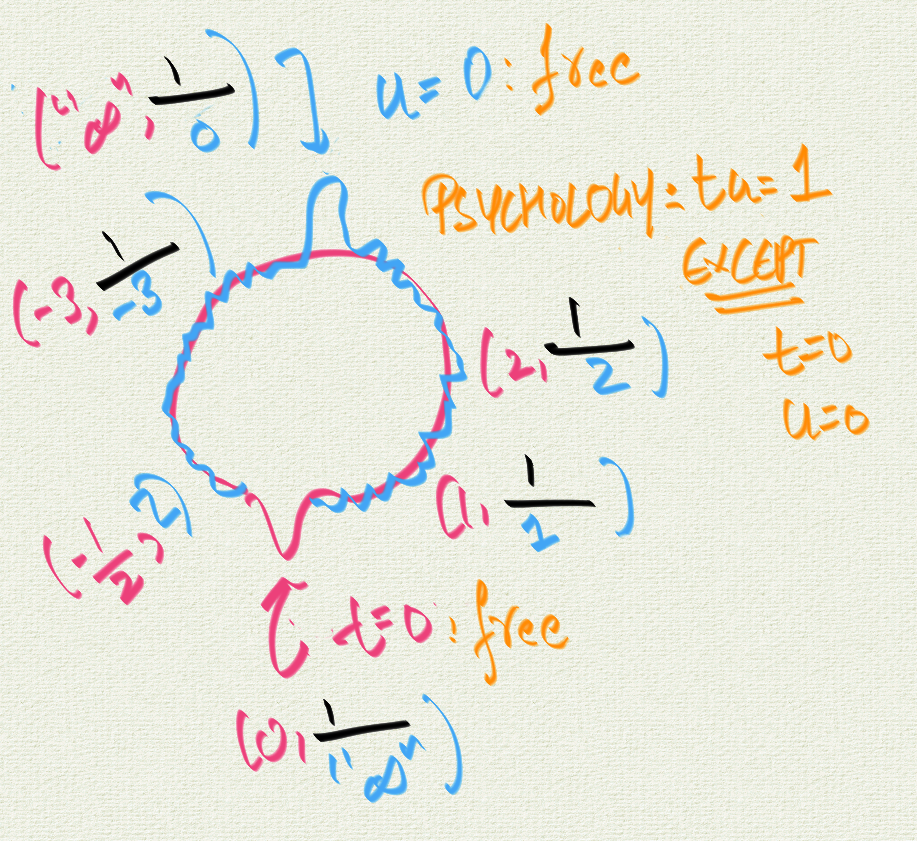
\includegraphics{projective-space-glued.png}


What are the points? in $\mspec$, we have the $t$-line, $\A^1 \simeq \C$,
and then we have the $u$ line, leaving out the point $u = 0$ [which is $t = \infty$].
So we have an extra "point at infinity", $\{ \infty \}$ which comes from
the unglued $u$. So we really have added a point at infinity!

In the scheme story, we really only have one extra point, the generic 
point of $t$, which is $[\{0\}]$, the point that is somewhere on that line.
This generic point of $t$ is glued to the generic point of $u$.


What are the functions on $\P^1_\C$? it's a function on $f(t) \in \C[t]$,
$g(u) \in \C[u]$ such that $f(t) = g(1/t)$  , the point that is somewhere on that line.
This generic point of $t$ is glued to the generic point of $u$.


What are the functions on $\P^1_\C$? it's a function on $f(t) \in \C[t]$ that
is everywhere except the north pole, and a function $g(u) \in \C[u]$ which
is defined everywhere other than the south pole. We need
to impose the condition that $f(t) = g(1/t)$ due to our gluing. The only such
functions we can build are going to be constants!

\section{Example: General projective space: $\P_k^n$}

The idea is that we have $(n+1)$ space and then we quotient by lines
through the origin. 

Just as we accepted $\P^1$ by thinking of lines through the ceiling,
we can think of higher projective spaces by lines through the ceiling,
lines through the left wall, lines through the right wall...

We start with $\A^n_k = \Spec k[x_{1/0}, x_{2/0}, \dots, x_{n/0}] = U_0$
where we psychologically think of  $x_{i/j}$ as $x_i / x_j$. To make
our notation nicer, we can just toss in $x_{0/0} = 1$ anyway, giving
us $U_0 = \Spec k[x_{0/0}, x_{1/0}, \dots, x_{n/0}$.
Similarly the standard open set $U_i = \Spec k[x_{1/i}, x_{2/i}, \dots, x_{n/i}]$.


Recall that we only need to glue pairwise gluing criteria, and
make sure that this works for all triples and we are done (This was apparently
an exercise. Go back and do it!)


To glue $U_i$ to $U_j$, we take:
\begin{align*}
&\Spec \left(k[x_{1/i}, x_{2/i}, \dots, x_{n/i}]/(x_{i/i} - 1) \right)_{x_{j/i}}
\leftrightarrow
\Spec \left(k[x_{1/j}, x_{2/j}, \dots, x_{n/j}]/(x_{j/j} - 1) \right)_{x_{i/j}}
\end{align*}

Now our notation will tell us to glue $x_{k/i} = x_{k/j}/x_{i/j}$. This
will "just work??" \textbf{TODO: need to check this!}

\section{Why does $\O(D(f)) = A_f$ define a sheaf?}
We want $\O(D(f)) = A_f$. We know that topologically, $D(f) \simeq \Spec A_f$.
Why is this well defined? Why does it give us sheaves over a base?


Define $\O(D(f))$ to be the localization of $A$ at the multiplicative subset
of those functions (elements of $A$) that vanish nowhere in $D(f)$. That is,
we are allowed to invert function $g$ such that $D(f) \subseteq D(g)$. 
Alternatively, this is the same as $V(g) \subseteq V(f)$. So we can invert
by functions which vanish only at points of $V(f)$.

For example, in $\spec k[x, y]$, for $\O(D(x, y))$, we are allowed to divide
by $x^7$ but not by $x + y$, because $x + y$ vanishes on $(1, -1)$ where $xy$
does not vanish. 

Most psychologically, we are only allowed to divide by things which 
are non-zero on $D(f)$. So on restriction to $D(f)$, the functions should
be non-zero.

The nice thing about this is that we are referring to $D(f)$ but not $f$
itself! The key thing to check is that this is the same as saying
$\O(D(f)) = A_f$. \textbf{TODO: Check this!}


\subsection{What do we need to check?}
We need to check that for any $D(f)$ covered by a bunch of $D(f_i)$'s 
we have the identity and gluability axioms.

The case $D(f) = \spec A$ is notationally simpler, but the proof
naturally generalizes to $D(f)$ of some arbitrary $f$.

\subsection{More generally}
If $M$ is an $A$-module we can define a sheaf of $\O$-modules in $\spec A$
in the same way called $\tilde{M}$. On $D(f)$ we define $\tilde{M}(D(f)) \equiv M_f$.

\section{Stalks of the structure sheaf of $\Spec A$}
The sheaf $\tilde{M}$ is a "quasicoherent sheaf", apparently.

If we have a point $[\p] \in \Spec A$ then $\O_p \simeq A_p$. 
Similarly, if $M$ is an $A$-module, then $\tilde{M_\p} = M_\p$. [WHY?]

\subsection{Happy algebra consequence}
We know that elements of the sheaf are determined by their stalks.
Let $M$ be an $A$-module. So it's a global section of $\tilde{M}$, the
sheaf of $A$-modules. We know that sections are defined by their
stalks. So $M = 0$ iff $M_\p = 0$ for all primes $\p \subseteq A$.

\section{Check the identity axiom}

If $\Spec A = \cup_i D(f_i)$, why is $A \rightarrow \pi A_{f_i}$ an injection?
\begin{aside}
Wow, that's a really slick way to rephrase the identity axiom!
\end{aside}
Recall that $\spec A = \cup_i D(f_i)$ iff $A = (f_i)$ [ideal generated by these]
iff $1 = \sum_i a_i f_i$.


Now our question can be translated to:
suppose we have $f_1, f_2, \dots f_n, a_1, a_2, \dots a_n \in A$ such that
$\sum_i a_i f_i = 1$.  We have a module $m \in M$ such that
$M \mapsto M_{f_i}$ sends $m \mapsto 0$. Why is $m = 0$?

$m/1 = 0$ in $M_{f_i}$. This means that $f_i^{b_i} m = 0$  in $M$ [$b_i$ for "big"].
$m = 1 m = (\sum_i a_i f_i)^{\sum_i b_i} m$. Now in the expansion, we will
have some $f_i^{b_i}$. But $f_i^{b_i} = 0$, so $m = 0$.

The idea is that $\sum_i a_if_i$ is a partition of unity [fuck this is gorgeous].
We are covering $m$ by a partition of unity.


\section{Check the gluability axiom}
Supposedly for experts, we just need to say "flat descent".  

\section{Next week}
Gluability? Projective varieties and schemes [the begininning of projective geometry]

\section{Questions}
\subsection{Quotes by conrad}
\begin{itemize}
\item We live as we dream, alone
\item I don't like work, no man does. But I like what is in the work. The chance
     to find yourself. But no other man can ever know. They can only see the mere show,
      and can never tell what it means.
\item Your strength is just an accident arising from the weakness of others
\end{itemize}
\subsection{How do we see things over the rational normal curve}
Let us consider $k[w, x, y, z] / (wz - xy, wy - x^2, xz - y^2)$. Why is
it a surface? Why is it reduced? We are claiming it's a surface (2D)
but we have a 4D thing quotiented by a 3D thing. So do we really need 3 equations?
turns out we do really need three equations. 

How do we see that this is reduced? How do we know it's a surface? Well,
we don't even know what dimension is yet. But as long as we agree that
the plane is dimension 2, then we do know that it is dimension 2 away
from $w = 0$. This will take care of everything except for the origin. So if
$\A^2$ is a surface, then we know that the cone better be a surface.


How do we know it is reduced (no nilpotents)? The crucial hint  is that we can write
it differently such that it is obviously an integral domain. We will
write it as $k[a, b]$  we want the subring of polynomials with a total
degree of a multiple of $3$. Then $w = a^3$, $x = a^2 b$, $y = ab^2$, $z = b^3$.
Then we can show that the previous ring is equivalent to this one.

Why do we need three equations? Geometry is telling us that something is
going on with the origin, because everywhere else, it is "nice". So let
us focus on the origin. In that local ring, if we compute $\m/\m^2$ we would
find that it is 4D not 2D, thereby posessing a 4D tangent space, because
we will have 4 differentials $dw, dx, dy, dz$. Now, the number of degree
2 monomials in 4 varibles is 10:

$$
aa ab ac ad
ba bb bc bd
ca cb cc cd
da db dc dd
$$

We want the upper triangular part.

So we have that $m^2$ mod $m^3$ is 10 dimensional. But the three equations
that we have are LI. So it's impossible to cut out \emph{something}.

\subsection{Why is it that $f$ is determined by its values if there are no nilpotents?}
if we have $f \in A$, the claim is that if we now $f \mod p$ for all $p$ then
we know $f$ as long as there are no nilpotents.

That is because of the fundamental fact that if we have $f \in A$ and we 
know that $f = 0 \mod p$ for all $p$, then we claim that it is nilpotent.
The intersection of all prime ideals in a ring is a nilradical.

\subsection{Why is the definition of $\P^1$ is a correct definition?}
if it walks like projective space and quacks like projective space...

The definition given as projective space works also as manifolds using
ceilings! 

Vakil does not think that this is the right definition of projective space.
The right definition of projective space is this: What is a map to
projective space?  It is the data of a line bundle in $n+1$ sections,
not all zero. Einsenbud and Harris goes through this in detail.

\subsection{When you write a scheme as the union of two principal open sets, is the $O$ of the union the categorical pullback?}
Yes, because that is exactly the sheaf condition.

\subsection{Why are we always dealing with triple intersection?}
Is there an analogy with Van Kampen? Descent is another word for gluing.
Sometimes we have to use double interesctions, sometime triple. For identity
we worry about singles, gluing we go to doubles.

Fundamental groups can be thought of in terms of covering spaces. The
fundamental group data of loops is the same as the deck transformations
of the covering space.

More generally, if we have a topological space and a surjective map to it.
If we know how to map into $U$ and $V$, there is extra information about
how they glue (???)

If there are three open sets, we need the conditions to not contradict
each other. $U \leftrightarrow V$, $V \leftrightarrow W$ should not contradict
with $U \leftrightarrow W$.


Since the covering space has the same data as the fundamental group,
assembing the covering space should feel the same as assembling the
fundamental group. 

The cocycle condition for gluing is the same as asking that the relation
becomes an equivalence relation (?)

\subsection{Is there a sense in which generic points encode homotopical/homological/global information?}
Over the generic point, all line bundles are trivial, because all line bundles
are locally trivial.

Take a curve and take two closed points, take the intersection of all
neighbourhoods of closed points. This should be a semi-local ring
because it has two maximal ideals corresponding to the two closed points.
If we look at $\mspec$ we see two points. If we see $\spec$ they are
connected by the generic points.

\subsection{How did we find the generic point on $\CP^1$?}
We had the original generic point of $\A^1$.We then set glued stuff together.
When we glue the two things, we need to show that the generic points glue.
Well, the idea is that since most of the points were glued together,
the generic point which is "everywhere but nowhere" also had glue on it,
as did the other generic point [lmao, this is hilarious]. So when
we glue them together, they are the same thing.


\subsection{Hartog's theorem}
In complex analysis. We have an analytic closed subset. It's codimension
is bigger than 1. Then any function defined on this subset  extends
over it.

\subsection{Defining the structure sheaf using distinguished open sets is different.}
But we can use compatibility of germs to build the full structure. So why
do we need open sets at all? We need to show that the sections over the
distinguished opens are what we say they are.

If we are given an element $A_p$ for all $p$ and they are compatible.
Why do they come from $A$? We need to glue!

\subsection{Two ways of gluging $\A^1$}
They are different as real topological spaces because the points $t = 0, u = 0$
have different neighbourhoods.

In the zariski topology, they are the same. But Zariski is too blunt. Once
we have the sheaf of rings, we can distinguish the spaces.

Zariski is deliberately blunt so we can carry information on the sheaf of
rings.


The correct definition of Haussdorf works for arbitrary topologies.

\chapter{AG with matrices}
\href{https://www.youtube.com/watch?v=1UvW5iTkbLw&feature=youtu.be&t=819}{Richard E Borcherds, AG 8, strong nullstellensatz, time 15:00}.

\section{Nilpotent Matrices}
Consider $M_n(k)$: all $nxn$ matrices over a field $k$. A matrix
is nilpotent if $M^n = 0$ where $n$ is the same dimension as the size
of the matrix. We can show that this is an ideal, call it $I$.

Another way to think of the condition is to think of a matrix $M$ with
\emph{variable/symbolic} entries $a_{11}, a_{12}, \dots a_{1n}, \dots, a_{nn}$. 
Now $M^n$ is another \emph{symbolic} matrix with entries as some (very messy!) degree $n$
homogeneous polynomial. Now the ideal $I$ is the zero set of these homogeneous
polynomials. So it's the ideal generated by $(M^n[1][1] = 0, M^n[1][1] = 0, \dots, M^n[n][n] = 0)$.


Now, is $I$ a radical ideal? That is, is $I = \sqrt{I}$? We clam it is not.
For example, consider the trace. The Trace of a nilpotent matrix is 0.
But the trace is $a_{11} + a_{22} + \dots a_{nn}$ which is homogeneous
of degree 1,\textbf{not} homogeneous of degree $n$. This, it belongs to
$\sqrt{I}$ but not to $I$.

Let us consider $n = 2$ concretely:

\begin{align*}
&A = \begin{bmatrix} 
&     a & b \\
&     c & d \end{bmatrix} \\
&A^2 = \begin{bmatrix} a^2 + bc & ab + bd \\ ac + cd & bc + d^2 \end{bmatrix} \\
&I = (a^2 + bc, a(b+d), c(a+d), d^2 + bc) \\
&Tr(A) = a + d
\end{align*}
Some power of $Tr(A) = a + d$ is in $I$. What is the smallest power of $(a+d)$
is in $I$? $(a+d)^2 \not \in I$ but $(a+d)^3 \in I$. It's not obvious that
$(a+d)^3$ ought to lie in $I$ at all!



\section{Commuting Matrices}

\end{document}
